\documentclass{template/openetcs_report}
% Use the option "nocc" if the document is not licensed under Creative Commons
%\documentclass[nocc]{template/openetcs_article}
\usepackage{lipsum,url}
\usepackage{supertabular}
\usepackage{multirow}
\usepackage{color, colortbl}
\usepackage{hyperref}
\usepackage{listings}
\usepackage{makeidx}
\definecolor{gray}{rgb}{0.8,0.8,0.8}
\usepackage[modulo]{lineno}
\usepackage{float}
\usepackage{fixme}
\usepackage{pdflscape}
\usepackage[acronym, % list of acronyms
  %section, % add the glossary to the table of content
            %description,% acronyms have a user-supplied description,
 style=longheader, % table style
 nonumberlist % no page number
  ]{glossaries}

\graphicspath{{./template/}{.}{./images/}}

\renewcommand*{\glspostdescription}{} %Deactivate point at the end of every description
\renewcommand*{\glossaryname}{Glossary}

%create glossary
 \makeglossaries
 %Glossary terms
 \loadglsentries{glossary}

\begin{document}
\frontmatter
\project{openETCS}

\newcommand{\define}[1]{\index{#1}\emph{#1}}






%Please do not change anything above this line
%============================

%user specified macros
%\newenvironment{activity}[2][planned]
	{\begin{tabular}{p{0.25\textwidth}@{\hspace{0.05\textwidth}}p{0.7\textwidth}}
			\multicolumn{2}{p{\textwidth}}{\colorbox{black}{\begin{minipage}{1.1cm}\begin{center}\textsc{\footnotesize \textcolor{white}{#1}}\end{center}\end{minipage}}~~\textbf{#2}}\\
	}
	{\end{tabular}}

\newcommand{\entry}[2]{#1:&#2\\}
\newcommand{\website}[1]{Website:&\url{#1}\\}
\newcommand{\desc}[1]{\multicolumn{2}{p{\textwidth}}{#1}\\}

\newcommand{\VV}{Verification \& Validation\xspace}
\newcommand{\vv}{verification \& validation\xspace}

\newcommand{\tbd}{\colorbox{cyan}{\%\%To Be Defined\%\%}}
\newcommand{\tbc}{\colorbox{cyan}{\%\%To Be Confirmed\%\%}}
\newcommand{\todo}[1]{\colorbox{cyan}{\%\%{#1}\%\%}}
\newcommand{\nthng}[1]{}

% The document metadata is defined below

%assign a report number here
%\reportnum{OETCS/WP3/D3.5.1.3}

%define your workpackage here
\wp{Work-Package 3: ``Modeling''}

%set a title here
\title{openETCS System Architecture and Design Specification}

%set a subtitle here
\subtitle{Third iteration: Scope of openETCS ITEA2 Functions}

%set the date of the report here
\date{November 2014}


%document approval
%define the name and affiliation of the people involved in the documents approbation here
\creatorname{Baseliyos Jacob}
\creatoraffil{DB Netz AG}

\techassessorname{[assessor name]}
\techassessoraffil{[affiliation]}

\qualityassessorname{Izaskun de la Torre}
\qualityassessoraffil{SQS}

\approvalname{Klaus-R\"udiger Hase}
\approvalaffil{DB Netz}


%define a list of authors and their affiliation here

\author{Baseliyos Jacob, Bernd Hekele, Peyman Farhangi, Stefan Karg, Valerio D´Angelo}

\affiliation{DB Netz AG\\
  V\"olckerstrasse 5\\
  D-80959 M\"unchen Freimann, Germany}

\author{Uwe Steinke}

\affiliation{Siemens AG}

\author{Christian Stahl}

\affiliation{TWT-GmbH}

\author{Jakob Gärtner}
\affiliation{LEA Engineering}

\author{Jos Holtzer, Jan Welvaarts, Vincent Nuhaan}
\affiliation{Nederlands Spoorwegen}

% define the coverart
\coverart[width=350pt]{openETCS_EUPL}

\newpage
%define the type of report
\reporttype{Architecture and Functional Specification}


\begin{abstract}
%define an abstract here
This document gives an introduction to the architecture of openETCS. The functional scope is tailored to cover the functionality required for the openETCS demonstration as a objecrive of the ITEA2 project. The goal is to demonstrate the proof of concept on the ETCS Level 2 Utrecht Amsterdam track with real scenarios. It has to be read as an add-on to the models in SysML, Scade and to additional reading referenced from the document.
\end{abstract}

%=============================
\maketitle

%Modification history
%if you do not need a modification history table for your document simply comment out the eight lines below
%=============================


\chapter*{Modification History}
\tablefirsthead{
\hline 
\rowcolor{gray} 
Version & Section & Modification / Description & Author \\\hline}
\begin{supertabular}{| m{1.2cm} | m{1.5cm} | m{6.6cm} | m{3.7cm} |}
0.1 & Document & Initial document providing the structure & Baseliyos Jacob \\\hline
0.2 & Document & Workshop Results included and some pretty-printing & Bernd Hekele\\\hline
0.3 & Document & Update of Design work, introduction and architecture & Baseliyos Jacob and WP 3 Team\\\hline

\end{supertabular}

% list subsubsections in table of contents
\setcounter{tocdepth}{3}


\tableofcontents
\listoffiguresandtables
\newpage
%=============================

%Uncomment the next line if you need line numbers for tracebility when the document is in review
%\linenumbers
%=============================


% The actual document starts below this line
%=============================

\mainmatter

\chapter{Introduction}


%-----------------------------------------------------------------------
%\subsection{Introduction}
%-----------------------------------------------------------------------
%\tbc
%
\section{Motivation}
%\tbc
	%BaseliyosJacob
	%additions / changes by JakobGärtner
The openETCS work package 3 (WP3) aims to provide – amongst others - the software architecture for the openETCS kernel in order to eventually build the software itself. 

The WP3  partners had by the end of 2014 put great effort in the openETCS software design, thus far without making definite choices on the software architecture itself respective of functional breakdown and data structures of the openETCS kernel. Since the project planning foresees in the production of a reference software to be used as a demonstrator by June 2015, it was of paramount importance that a first design delivarable of the openETCS kernel architecture be finalized shortly but no later than November 2014.\\

In compliance with the agreements made during the last WP 3 meeting at the 10.09.2014 in Brussels, DB has taken the initiative to design the aforesaid architecture including of functional breakdown and data structures in order to safeguard a timely delivery of these products. Furthermore, DB has ensured that these developments are focused on including end user requirements so as to develop a design in conformity with the needs and requirements of the operators. Specialists of DB and NS have cooperated together with other partners in WP3 to produce the main concepts of the system .\\

In Novermber 2014, DB has invested by adding an external embedded software specialist in order to fully profit from the decisions that lead to the consolidation of the openETCS toolchain and to set up a design process that would lead to a first demonstration in March 2015\\

This document shows a snapshot of the software and will also give an outlook to the scope of the next iteration and the final objectives.\\


\section{Objectives}
%\tbc
%Baseliyos Jacob
The prime objective of WP3 is to produce a fully formal prototype for the openETCS reference system that can function as a demonstrator in collaboration with WP 4 and WP 5  for the openETCS approach and will be used as such in the final phase of the project. That phase is the first half of 2015.  This objective is defined as … 

\textbf{High level Objectives of this work:}
<<any further general statements on the ITEA2  objectives, like…>>\\

\begin{itemize}
\item Work on a model bases approach and process for effective collaborative work within an international ETCS developer team as stated above, the project needs a definite architecture design by the end of 2014.

\textbf{This document targets:}
\item Defining the general design and conditions of the openETCS architecture, functional breakdown and data structures
\item Providing the guidelines for discussion during the workshops that are planned in October and November 2014 that will result in the final and decisive version of this document
\item Being the ‘platform’ for finalization i.e. whatever be the products or results of the workshops shall be integrated in this document.

\textbf{Apart from these general objectives, the document means to provide for the materials that will enable WP3 partners to improve the efficiency of the Work Package activities:}
\item The comprehensive architecture design shall enable splitting the work load according to the building blocks defined by the architecture and allocate strictly compartmented work parcels or activities to WP3 partners.
\item Doing so will enable WP3 to avoid any double work
\item  Compartmenting the work load according to the functional building blocks as defined by the architecture will enable efficient planning of activities, be it individually or the integrated WP3 planning for the coming period, aiming at a just in time delivery of all results and products
\item  Compartment the work load according to the functional building blocks as defined by the architecture will enable efficient planning of activities, be it individually or the integrated WP3 planning for the coming period, aiming at a just in time delivery of all results and products
\end{itemize}

%\tbc
%JakobGärtner


\section{Scope of deliverables}

The prime original objective of WP3 was to produce a rapid prototype for the openETCS reference system that can function as a demonstrator in collaboration with WP 4 and WP 5  for the openETCS approach and will be used as such in the final phase of the project. That phase is the first half of 2015. \\

We have to see this original objective in the context of the overall innovation promise of openETCS and the related exploitation potential.
Taking into account the current situation of the project (as of Nov. 2014) we have to make choices that make sure that the remaining budget and resources are wisely used, which necessitates that the WP3 deliverables become more "multi- purpose":

 •  provide a functional formal specification of openETCS, based on functional analysis, and traceable to the SRS.
 
 •  Iteratively develop the software architecture and design description document (ADD) while using the formal specification as an executable functional model
 
 •  Utilise real- world use-case scenarios as early as possible in the development process
 
If we take this approach, we can use the iterative development method, while applying a pragmatic view of SCRUM (which has been defined as the high- level project management method for this project) in order to build the following deliverables:

 •  An ADD document, providing a functional description of software architecture and design.
 
 •  A RFC (Request For Comment) process that provides a cross- reference to the SRS, listing all requirements and design conflicts that have been identified during our work
 
 •  A formal, executable model of the openETCS kernel, which can directly be used as entry point into a (future) EN5012x SIL4 compliant software design process, as well as functional reference during simulation and on the planned WP5 demonstrator.
 
 
\begin{figure}
  \centering
  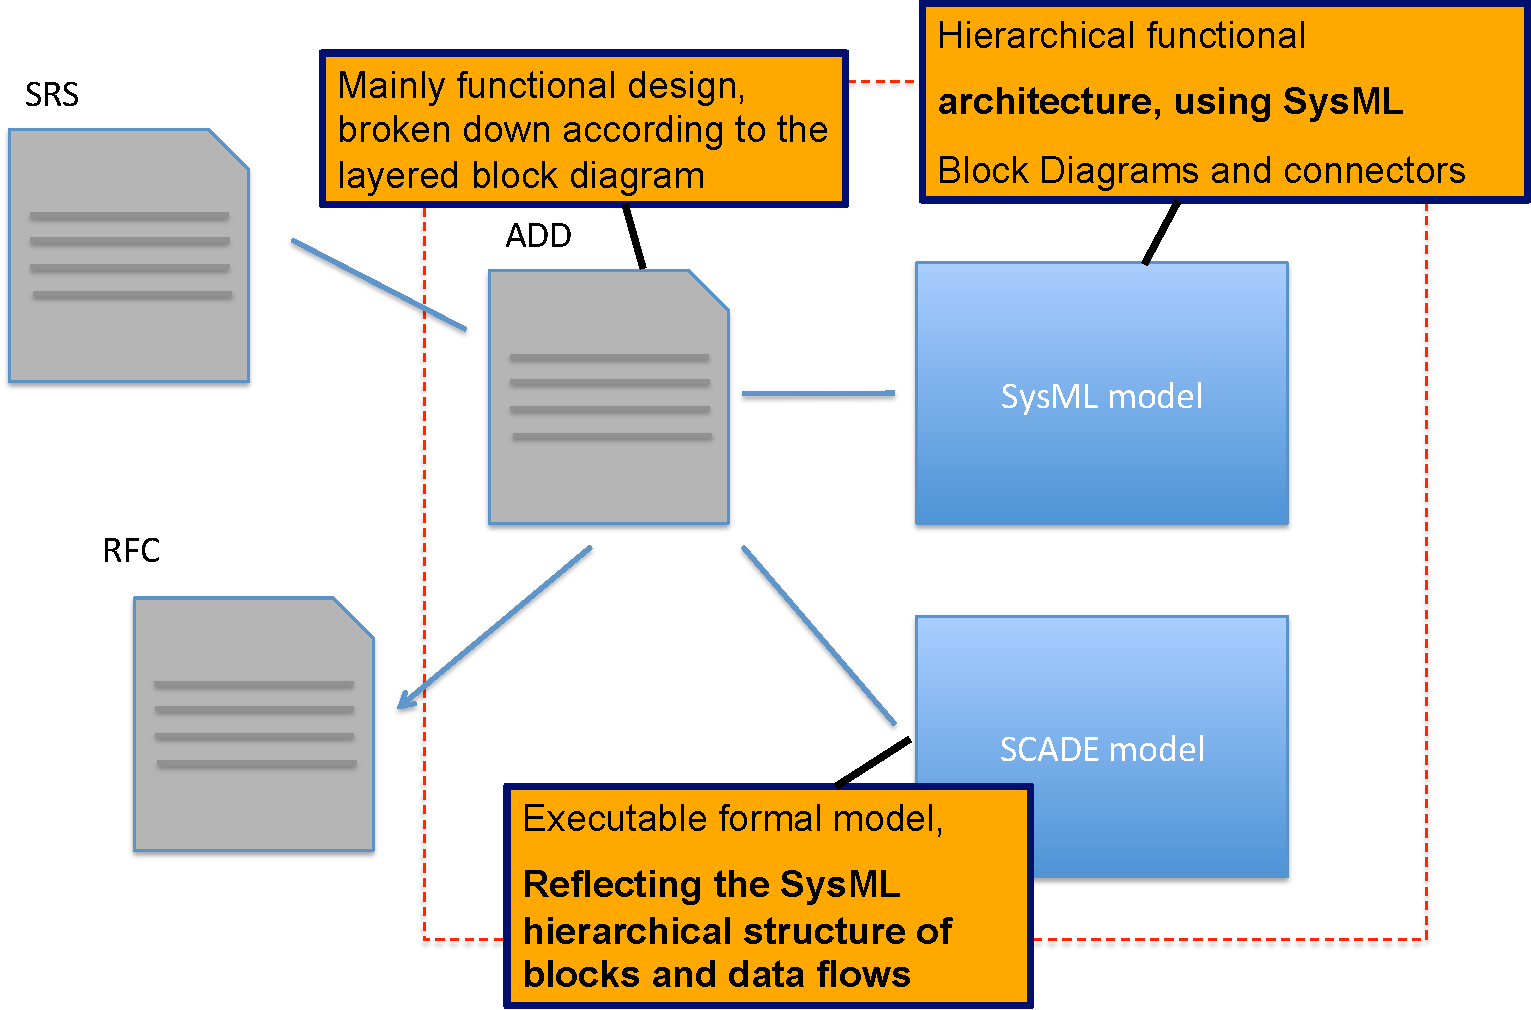
\includegraphics[width=\linewidth]{document-relations.pdf}
  \caption{Document relationships in WP3}
  \label{fig:doc-rels}
\end{figure}

Each main WP3 collateral has it's distinct role in the overall project structure. For a schematic view of the dependencies, see figure \ref{fig:doc-rels}. \\


\textbf{Scope of the ADD document (this document)}\\

 



The ADD document is intended to provide the following main information:

• Internal guidance for the project: Provide authoritative guidance on process, responsibilties, process and workflow.\\
 
• Architectural design description: Provide complete information on the overall architecture of the openETCS kernel functions.\\

• Functional design description: Provide comprehensive information on the design of the system, which includes QoS aspects, interfaces, data types, algorithms and finally the full software design.\\
\\

The nature of the development process implies that this document will be a "living document", meaning that it will be constantly updated, with new iterations being planned as follows:

•  Intermediate work iterations (0.x): as required until the ITEA2 intermediate review (March 2015)

• First main release (1.0): as a deliverable for the ITEA2 intermediate review (March 2015)

• Intermediate work iterations (1.x): as required until the demonstrator milestone (June 2015)

•  Second main release (2.0): for the demonstrator milestone (June 2015)

•  Intermediate work iterations (2.x) for the rest of the project duration (until Oct 2015)

•  Final release (3.0) for the final review.

Intermediate work iteration shall be managed using the normal day-to-day pull/ review process, while main releases require a formal document sign-off.\\

\textbf{Scope of the User Validation Scenarios}\\

The work of WP3 has now been aligned to the milestones that are relevant for the overall project:

•  (1) ITEA2 intermediate review (March 2015)

•  (2) Demonstrator milestone (June 2015)

•  (3) Final review (End of 2015)

In order to support the functional approach, we use operational scenarios that are described the the User Validation Scenario Document.

These are based on the following data:

•  Rules from NS for the operation of trains

•  Infrastructure data from the Utrecht- Amsterdam line

In order to support the functional analysis, which is aligned with the project's milestones, this document will define use cases along the following principles:

•  (1) Selected operational scenarios on selected sections of the Utrecht- Amsterdam track

Based on nominal scenarios, our simulated train will drive across actual (simulated) infrastructure, selecting only a few, typical balise groups.
This will allow WP3 to implement the relevant mode/level/message (balise and RBC) functionality first,

The openETCS kernel model has been complemented by a simple DMI representation, in order to validate actual behaviour. 

In march 2015, only basic scenarios will be demonstrated, which have been organised as use cases, based on a plant/ controller co-simulation concept.

The future 


•  (2) Selected operational scenarios on the full Utrecht- Amsterdam track

Based on nominal scenarios, our simulated train will drive across actual (simulated) infrastructure, covering the entire Utrecht- Amsterdam track.
This will allow WP3 to implement the relevant mode/level/message (balise and RBC) functionality first, fo full functional coverage of the test track.

Compared to the fist step in March, we will also cover more operational scenarios according to the NS operational rules.

A generic, interactive simulation concept will be created for this purpose. 

The entire track with its 488 balise groups and known (real) RBC messages as well as specific validation scenarios will be modelled.

A presentation of this concept can be found in the section "Dynamic Simulation".

•  (3) Full coverage of Utrecht- Amsterdam

For the final review, we will prepare a openETCS kernel software that can run defined scenarios, accordiing to the NS operation regulation, across the entire Utrecht- Amsterdam line, either replaying actual train rides or simulating various events, nominal and non- nominal.

In cooperation with WP4 and WP5 this will provide additional input for demonstration and validation.



\textbf{Scope of the RFC process}\\


The RFC document is a deliverable that was added to the WP3 set of documents during the Nov 3-7, 2014 Munich workshop.\\

Most (industrial) ETCS OBU systems have been built based on pure SRS analysis. at least in theory. In practise, each implementation is derived from the SRS, but with a mindset that is partially driven by the company culture and local operational regulation prior to ERTMS introduction.\\
This has lead to a plethora of ETCS systems, which exhibit subtle differences which lead to incomplete compatibility between OBUs and track equipment of different suppliers. Each OBU works best on a track which was built by the same supplier in the same country.\\
One of the objectives of openETCS is to provide a reference design for an ETCS UBU that reduces these variations.\\
The experts of WP3 and WP4 agree that a functional approach will lead to a better understanding of the system. As the SRS remains the formal reference, we have to provide formal feedback which is traceable to the SRS.\\
This is the objective of the RFC document.

The RFC document shall be structured following the paragraphs in the SRS and shall provide full traceability to the openETCS ADD.
Each design decision that can be traced to a deviation from the SRS or that highlights inconsistencies inside the SRS shall be documented in the RFC.\\
The RFC is hence a deliverable that provides formal feedback to the relevant ERTMS stakeholders.\\

(we still have to discuss the precise interaction between the SRS Analysis effort, WP4 and this RFC document)

The nature of the development process implies that this document will be a "living document", meaning that it will be constantly updated, with new iterations being planned as follows:

•  Intermediate work iterations (0.x): as required until the ITEA2 intermediate review (March 2015)

• First main release (1.0): as a deliverable for the ITEA2 intermediate review (March 2015)

• Intermediate work iterations (1.x): as required until the demonstrator milestone (June 2015)

•  Second main release (2.0): for the demonstrator milestone (June 2015)

•  Intermediate work iterations (2.x) for the rest of the project duration (until Oct 2015)

•  Final release (3.0) for the final review.

Intermediate work iteration shall be managed using the normal day-to-day pull/ review process, while main releases require a formal document sign-off.\\


\textbf{Objectives and scope related to formal executable model}\\

During the previous iterations of this document, it was proposed to use a traditional waterfall model in order to define the architecture and subsequently the functional and software design of the openETCS kernel software.
We have now shifted the design paradigm to a more agile process, where we will use iterations (functional analysis, implementation of prototype formal executable model, refinement) in order to design the software modules. (bottom- up design of modules)\\
These will then be merged into a top- down architecture by the chief architect, using best practises that are well established for data- flow oriented software designs.\\

The result will be a functional, formal model, from which code can be generated that implements the functionality fin an hardware- independent way.\\
This code is hardware- and platform agnostic and can be integrated with the openETCS runtime environment, which is adaptable to different system architectures and APIs.\\



\section{Roles, responsibilities and tasks}
%\tbc
%Baseliyos Jacob
\textbf{In this section, the roles and responsibilities of the WP3 partners are confirmed, especially where they divert from what has been agreed upon at the start of WP3:}

\begin{itemize}
\item\textbf{Responsibilities} First of all, in the last WP 3 meeting in Brussels on  10.09.2014 DB proposed to take over the lead of the architecture design and functional breakdown. At the subsequent weekly scrum meeting on 12.09.2014,  it was agreed upon by all participants that DB will take over the lead (see Appendix … );\\
\item\textbf{Planning:} Alstom as WP 3 leader will remain to be responsible for the planning and the allocation of the defined tasks to the different partners\\
\item\textbf{Roles:} Alstom will also coordinate the work and safeguard that the defined results will be delivered according to the quality requirements that are agreed within the ITEA2 project and the schedule and the milestones that will be agreed upon during the coming workshops;\\
\item All WP3 partners will deliver the results or products according to planning as will be agreed upon during the said workshops. \\

In the interest of a swift production of the critical documentation of which this version is a draft, specific tasks will be defined in terms of concrete results to be delivered, the timeframes in which these results must be produced and the partner who shall be responsible for that specific result and the planning. This is to safeguard the timely delivery. The process will be described in the next sections.\\
\end{itemize}



%\tbc
%JakobGärtner for the chapter on openETCS design process



\section{openETCS Design Process}


\subsection{SRS- Driven Approach vs. Functional Approach}

Most attempts to formalise the ETCS onboard software have been focusing on creating models that were directly mirroring the SRS specification.
While this gives a full picture of the status quo of the SRS, it is not sufficient in order to fully understand the main issues that stem from the approach by which the SRS was conceived. \\
%
The SRS is aiming in what could be called the quadrature of the circle:
\begin{itemize}
\item Define a common specification of all aspects of the requirements of the ETCS system (Basic System Description, Principles, Functionality, Procedures and Application Level Communication Protocols, amongst others)
\item Create a framework that is compatible with all the local ways of driving trains
\item Ensure a framework for simple interoperability 
\item Give a full understanding of the wayside and onboard views of the system
\end {itemize}

Instead of building yet another copy-paste direct formalisation of the ETCS SRS, we are proposing a different approach:
%
\begin{itemize}
\item Functional analysis of the SRS
- onboard point-of view
- SRS driven
- Focused on the reference track (ETCS L2 Utrecht- Amsterdam)
\item Formalisation
- Executable formal model (using SCADE tool suite)
- Dynamic simulation 
\item Validation
- interface to WP4
\end{itemize}

Together with the document structure described above, this will for the first time lead to a OBU- centric formalisation of the SRS, with systematic Change Request process (through our RFC approach) and a functional reference that can be used to validate ETCS OBU software as well as wayside implementations once it is completed.\\

\subsection{Top- down vs. Bottom- Up}
%
%
The functional approach, together with other considerations mandated a combined top-down/ bottom up design approach.
While the basic architecture was derived from existing architectures, with basic concepts and functional breakdown derived from the existing implementations of the WP3 leader, the actual functional analysis and the related software design was built bottom- up.\
Thanks to the model- based formal design approach, the components could then be seamlessly merged with the top- down architecture.\
Using this approach, the system and software architecture was at a relatively immature approach when we split the work in order to separately analyse and design the different functional blocks of the system. \
The openETCS agile approach allows to iteratively integrate and align the top- down architectural view with the separately developed main functional blocks.\


\subsection{Working groups}
%
%
While the basic architectural concept has been driven jointly by Alstom, DB and NS, the analysis and design of the functional blocks was distributed into working groups.
Each working group consists of a combination of application/ analysis specialists and software/ SCADE specialists.\\

\subsection{Use- case driven setting of priorities}
%
%
In order to focalise the work and to ensure our functional approach, DB has taken the role of product owner. 
As a reminder: in an agile/ SCRUM project management approach, the product owner has the responsibility to represent the interests of the customer.
The goal being to prove the openETCS concept and model on the ETCS L2 Utrecht- Amsterdam line, DB is formulating a set of at first very basic, then advanced and towards project completion comprehensive and complete scenarios and requirements for demonstration. \\
In- line with agile project management methodology, these requirements are presented to the WP3 team in the form of "user stories" which help to drive the project priorities. \\

\subsection{integration}
%
%
Integration on openETCS context is focusing on several aspects:
\begin{itemize}
%
\item Integration of SCADE functional blocks with overall SCADE architectural model
%
In a SCADE context, model-to-model integration is straightforward. As each functional block has a clear interface and all blocks have identical semantics we could follow an iterative, constructive and agile approach.
Integration was mainly driven by alignment of interfaces and validated by interactive simulation. 
%
%
\item Integration of openETCS model with WP3 simulation environment 
%
For the March 2015 ITEA review, a simple dynamic simulation environment was set up using SCADE tools (SCADE Display to build a first version of an openETCS DMI software, SCADE Rapid Prototyper to interact with the simulator).
Integration of the openETCS OBU software model followed the same principles as model-to-model integration.
The same concept will be extended for a full dynamic simulation of the Utrecht-Amsterdam line in interaction with the openETCS reference model.
%
%
\item Integration of openETCS model with openETCS runtime
%
Currently, the demonstration is purely on model/ simulation level. However, since the openETCS toolchain allows for automatic code generation, we will integrate the generated code with the openETCS runtime. 
As the generated code is strictly target agnostic, integration can be adapted very flexibly to different hosts and execution models.
Details of this integration phase will be discussed in the final version of this document, a first overview is given in the section discussing the APIs.
%
%
%\item Integration on EVC/ openETCS OBU
%
%The actual hardware integration 
%  ---------(this item is deferred for now// Jakob)
%
\end{itemize}

\subsection{Towards EN50128 SIL4 objectives, interface to WP4}

One of the objectives of openETCS is to demonstrate feasibility of the approach and concept in a CENELEC context.
While we are focusing on analysis and design for now, we will also formulate a certification strategy.

An actual EN50128 certification of the openETCS software is beyond the scope of this project.


%
% The following section commented out.
%
%REASON: this is/was an internal directive 


%\section{Assumptions and preconditions}
%\tbc
%Baseliyos Jacob
%\begin{itemize}
%\item All future contributions shall be fully aligned an compliant the finalised and approved document 
%\item Alls documents produced by the partners are requested to be compliant and merge to this document; other contributions will be discarded
%\textbf{The workshops are all about working as swift, as efficient and as productive as possible and make full use of the potential made available for these workshops by the partners. It is expected that the partners in the workshops will have the express intention to:}
%\item Contribute to the workshops with the intention to finalise the openETCS architecture;\\
%\item Provide resources according to the agreements made prior to the Workshops;\\
%\item Focus primarily on  getting concrete results regardless of methodological issues that might arise. Where necessary or opportune, classical project management methodology will be applied;\\
%\item Provide full transparency with respect to experience, knowledge base and information touching the subjects to be treated in the workshops;\\
%\item Document on paper or electronically all output of the workshops and integrate these with the underlying document;\\
%\item Restrict discussions only to topics that have an immediate impact on the content or the quality of the end product: the improved version of this document.\\
%\end{itemize}

\section{openETCS history and iterations}
%\tbc
%BaseliyosJacob
The openETCS Architecture and Design is beingimplemented in iterations. The current step (third iteration) is implementing essential kernel functions of the ETCS system. 
For a better understanding of the scope the Iteration is described in the following.

\textbf{Third Iteration Functional Scope: The OBU functions for Szenarios defined in chapter 3}

The openETCS third iteration model is defining the architecture and design of the openETCS OBU software. 
It is referencing  \cite{subset-026} UNISIG Subset\_026 version\_3.3.0. 

The appropriate functionality has been divided into a number of functional blocks that are being analysed and designed by work groups (as described in the previous section of this document).

The third iteration of the openETCS modelling effort is focusing on demonstrating some simple scenarios on the actual (for now simulated) Utrecht- Amsterdam infrastructure.

=======
%-----------------------------------------------------------------------
%\subsection{Mode and Level}
%-----------------------------------------------------------------------
%\tbc
%

\section{Motivation}
%\tbc
%BaseliyosJacob
The openETCS work package 3 (WP3) aims to provide – amongst others - the software architecture for the openETCS kernel in order to eventually build the software itself. WP3  partner has put great effort in the openETCS software design, thus far without making definite choices on the software architecture itself respective of functional breakdown and data structures of the openETCS kernel. Since the project planning foresees in the production of a reference software to be used as a demonstrator by June 2015, it is of paramount importance that a first design delivarable of the openETCS kernel architecture be finalized shortly but no later than November 2014.\\

In compliance with the agreements made during the last WP 3 meeting at the 10.09.2014 in Brussels, DB has taken the initiative to design the aforesaid architecture including of functional breakdown and data structures in order to safeguard a timely delivery of these products. Furthermore, DB has ensured that these developments are focused on including end user requirements so as to develop a design in conformity with the needs and requirements of the operators. Specialists of DB and NS have cooperated together with other partners in WP3 to produce this document.\\

As referred to above, the architecture description has to be finalized in the month of November 2014. This version of the document is a draft version, demonstrating the general directions and philosophy of the architectural design, the functional breakdown of the software and the data structures. The design is focused on maximum efficiency in order to maximize on RAMS performance of the end product.\\


\section{Objectives}
%\tbc
%Baseliyos Jacob
The prime objective of WP3 is to produce a fully formal prototype for the openETCS reference system that can function as a demonstrator in collaboration with WP 4 and WP 5  for the openETCS approach and will be used as such in the final phase of the project. That phase is the first half of 2015.  This objective is defined as … 

\textbf{High level Objectives of this work:}
<<any further general statements on the ITEA2  objectives, like…>>\\

\begin{itemize}
\item Work on a model bases approach and process for effective collaborative work within an international ETCS developer team as stated above, the project needs a definite architecture design by the end of 2014.

\textbf{This document targets:}
\item Defining the general design and conditions of the openETCS architecture, functional breakdown and data structures
\item Providing the guidelines for discussion during the workshops that are planned in October and November 2014 that will result in the final and decisive version of this document
\item Being the ‘platform’ for finalization i.e. whatever be the products or results of the workshops shall be integrated in this document.

\textbf{Apart from these general objectives, the document means to provide for the materials that will enable WP3 partners to improve the efficiency of the Work Package activities:}
\item The comprehensive architecture design shall enable splitting the work load according to the building blocks defined by the architecture and allocate strictly compartmented work parcels or activities to WP3 partners.
\item Doing so will enable WP3 to avoid any double work
\item  Compartmenting the work load according to the functional building blocks as defined by the architecture will enable efficient planning of activities, be it individually or the integrated WP3 planning for the coming period, aiming at a just in time delivery of all results and products
\item  Compartment the work load according to the functional building blocks as defined by the architecture will enable efficient planning of activities, be it individually or the integrated WP3 planning for the coming period, aiming at a just in time delivery of all results and products
\end{itemize}

\section{Roles, responsibilities and tasks}
%\tbc
%Baseliyos Jacob
\textbf{In this section, the roles and responsibilities of the WP3 partners are confirmed, especially where they divert from what has been agreed upon at the start of WP3:}

\begin{itemize}
\item\textbf{Responsibilities} First of all, in the last WP 3 meeting in Brussels on  10.09.2014 DB proposed to take over the lead of the architecture design and functional breakdown. At the subsequent weekly scrum meeting on 12.09.2014,  it was agreed upon by all participants that DB will take over the lead (see Appendix … );\\
\item\textbf{Planning:} Alstom as WP 3 leader will remain to be responsible for the planning and the allocation of the defined tasks to the different partners\\
\item\textbf{Roles:} Alstom will also coordinate the work and safeguard that the defined results will be delivered according to the quality requirements that are agreed within the ITEA2 project and the schedule and the milestones that will be agreed upon during the coming workshops;\\
\item All WP3 partners will deliver the results or products according to planning as will be agreed upon during the said workshops. \\

In the interest of a swift production of the critical documentation of which this version is a draft, specific tasks will be defined in terms of concrete results to be delivered, the timeframes in which these results must be produced and the partner who shall be responsible for that specific result and the planning. This is to safeguard the timely delivery. The process will be described in the next sections.\\
\end{itemize}



\section{Assumptions and preconditions}
%\tbc
%Baseliyos Jacob
\begin{itemize}
\item All future contributions shall be fully aligned an compliant the finalized and approved document 
\item Alls documents produced by the partners are requested to be compliant and merge to this document; other contributions will be discarded
\textbf{The workshops are all about working as swift, as efficient and as productive as possible and make full use of the potential made available for these workshops by the partners. It is expected that the partners in the workshops will have the express intention to:}
\item Contribute to the workshops with the intention to finalize the openETCS architecture;\\
\item Provide resources according to the agreements made prior to the Workshops;\\
\item Focus primarily on  getting concrete results regardless of methodological issues that might arise. Where necessary or opportune, classical project management methodology will be applied;\\
\item Provide full transparency with respect to experience, knowledge base and information touching the subjects to be treated in the workshops;\\
\item Document on paper or electronically all output of the workshops and integrate these with the underlying document;\\
\item Restrict discussions only to topics that have an immediate impact on the content or the quality of the end product: the improved version of this document.\\
\end{itemize}

\section{openETCS history and iterations}
%\tbc
%BaseliyosJacob
The openETCS Architecture and Design willb de documented and implemented in iterations. 

\begin{itemize}
\item \textbf{first iteration can be downloaded under the following link:}
\end{itemize}


\begin{itemize}
\item \textbf{second iteration has not been published due some technical issues and will fully substituted by the third iteration.}
\end{itemize}

\begin{itemize}
\item \textbf{first iteration can be downloaded under the following link:}
\end{itemize}
The current step (third iteration) is based on a step to implement the kernel functions of the ETCS system. For a better understanding of the scope the Iteration is described in the following.

\textbf{Third Iteration Functional Scope: The OBU functions for ccenarios defined in chapter 3}

The openETCS third iteration architecture and the design of the openETCS OBU software are derived from \cite{subset-026} UNISIG Subset\_026 version\_3.3.0. 

All these functions are object of the openETCS project and have to be analysed from their requirements and subsequently modelled and implemented. With the given manpower in WP 3, a reasonable selection and order of these functions is required for the practical work that allows the distribution of the workload, more openETCS participants to join and leads to an executable---limited---kernel function as soon as possible. 




\glsaddall
\printglossaries

\chapter{Input documents}
%-----------------------------------------------------------------------
%\subsection{Mode and Level}
%-----------------------------------------------------------------------
%\tbc
%Baseliyos Jacob
\textbf{This paragraphs gives an overview about the input doducments used for the:}
\begin{itemize}
\item Analysis of the OBU Functions
\item Functional decomposition and allocation of macro- and microfunctions
\item Design of the OBU Functions
\item Determination of "Use Cases" and Szenarios for the different iteration of the Architecture and Design Document
\end{itemize}

\section{Document x}

\section{Document x}

\section{Document x}

\section{Document x}

\section{Document x}

\chapter{Use case description - proof of concept Utrecht - Amsterdam}
%-----------------------------------------------------------------------
%\subsection{Mode and Level}
%-----------------------------------------------------------------------
%\tbc
%Baseliyos Jacob

\section{Proof of concept on the Track Utrecht Amsterdam User Stories 1 - 4}

The goal of the openETCS@ITEA2 project is to deliver at the and a proof of concept in a lab on a real ETCS Track. Since the Level 2 Utrecht - Amsterdam track was evaluated as the most approriate reference track for this concept due the maturity and representative of the track, it will be use for the mentioned simulation.\\

To start with the realisation of the concept in a iterative way in the same pattern the industry is proceeding and an regarding the "classical" state of the art of sytemanalisiys we started in this third iteration with the following Use Cases and Scenarios:\\

\subsection{Use Case and Scenario 1}
\textbf{Start of Mission - Awakening of the Train:}
This use case according to the procedure in chapter 5 will demonstrate the start of a train from a no power modus to the state that train will be ready for level and mode change according to the chapter 5.\\ 
Link on Git-Hub \url{https://github.com/openETCS/modeling/issues/66}

The following Subsystems needs to be realised for Scenario 1:\\
\begin{itemize}
\item Procedure
\item TIU Management
\item DMI Management and Controller
\item Position Report
\item Management of Radio Communication
\item Manage Track Data
\item Manage Mode and Level
\item Train Supervision
\end{itemize}

\subsection{Use Case and Scenario 2}
\textbf{Start of Mission - Start in Level 2 Mode FS:}
This use case according to the procedure in chapter 5 will demonstrate the start of a train from the awakening of the train in mode stand by to the state that train will receive a movement authority in level 2 and change into the mode full supervision to start running under real supervision according to the chapter 5.\\ 
link on Git-Hub \url{https://github.com/openETCS/modeling/issues/67}

The following Subsystems needs to be realised for Scenario 2:\\
\begin{itemize}
\item Procedure
\item TIU Management
\item DMI Management and Controller
\item Position Report
\item Management of Radio Communication
\item Manage Track Data
\item Manage Mode and Level
\item Train Supervision
\end{itemize}

\subsection{Use Case and Scenario 3}
\textbf{Brake intervention - Revocation of a Movement Authority and Overrun Permitted Speed:}
This use case according to the subset 26 chapter 3 principles will demonstrate the brake intervention that will cause by a revocation of a movement authority due to a occupied section or track an due simple overrun of a permitted speed  according to the chapter 3.\\ 
Link on Git-Hub \url{https://github.com/openETCS/modeling/issues/68}

The following Subsystems needs to be realised for Scenario 3:\\
\begin{itemize}
\item Procedure
\item TIU Management
\item DMI Management and Controller
\item Position Report
\item Management of Radio Communication
\item Manage Track Data
\item Manage Mode and Level
\item Train Supervision
\end{itemize}

\subsection{Use Case and Scenario 4}
\textbf{ETCS Onboard Unit is reading and sending track information:}
This use case according to the subset 26 chapter 3 principles will demonstrate the full completeness and checking the reading and sending of track information in interaction with the ETCS Onboard Unit and the track that will be separated in radio and balise messages. Messages and packages are defined in chapter 7 and 8 of the subset 26.\\ 
Link on Git-Hub \url{https://github.com/openETCS/modeling/issues/69}

The following Subsystems needs to be realised for Scenario 4:\\
\begin{itemize}
\item Procedure
\item TIU Management
\item DMI Management and Controller
\item Position Report
\item Management of Radio Communication
\item Manage Track Data
\item Manage Mode and Level
\item Train Supervision
\item Building of coordinate system
\end{itemize}

\section{Environment model for the use case demonstrations}

%
% nice screenshots needed!
%
%

In order to dynamically explore and demonstrate the openETCS OBU kernel software, a dynamic simulation and demonstration environmental model is being created.
During Iteration 3, this comprises the following features and functionalities:\\
•   openETCS OBU formal model \\
•   openETCS DMI formal model with Display specification model\\
•      Simplified version, not all features are implemented yet; following our use- case driven approach we are only implementing features that are essential to show the use cases selected by our "internal customer".\\
•    Environment model with \\
•  	- simplified track model (balise locations, speed profile)\\
•  	- simplified model of Movement Authority\\
•  	- interactive widgets to manipulate the simulation environment\\
\\
\\
\\


(see Figure \ref{fig:WP3-demo}.)
	
\begin{figure}
  \centering
  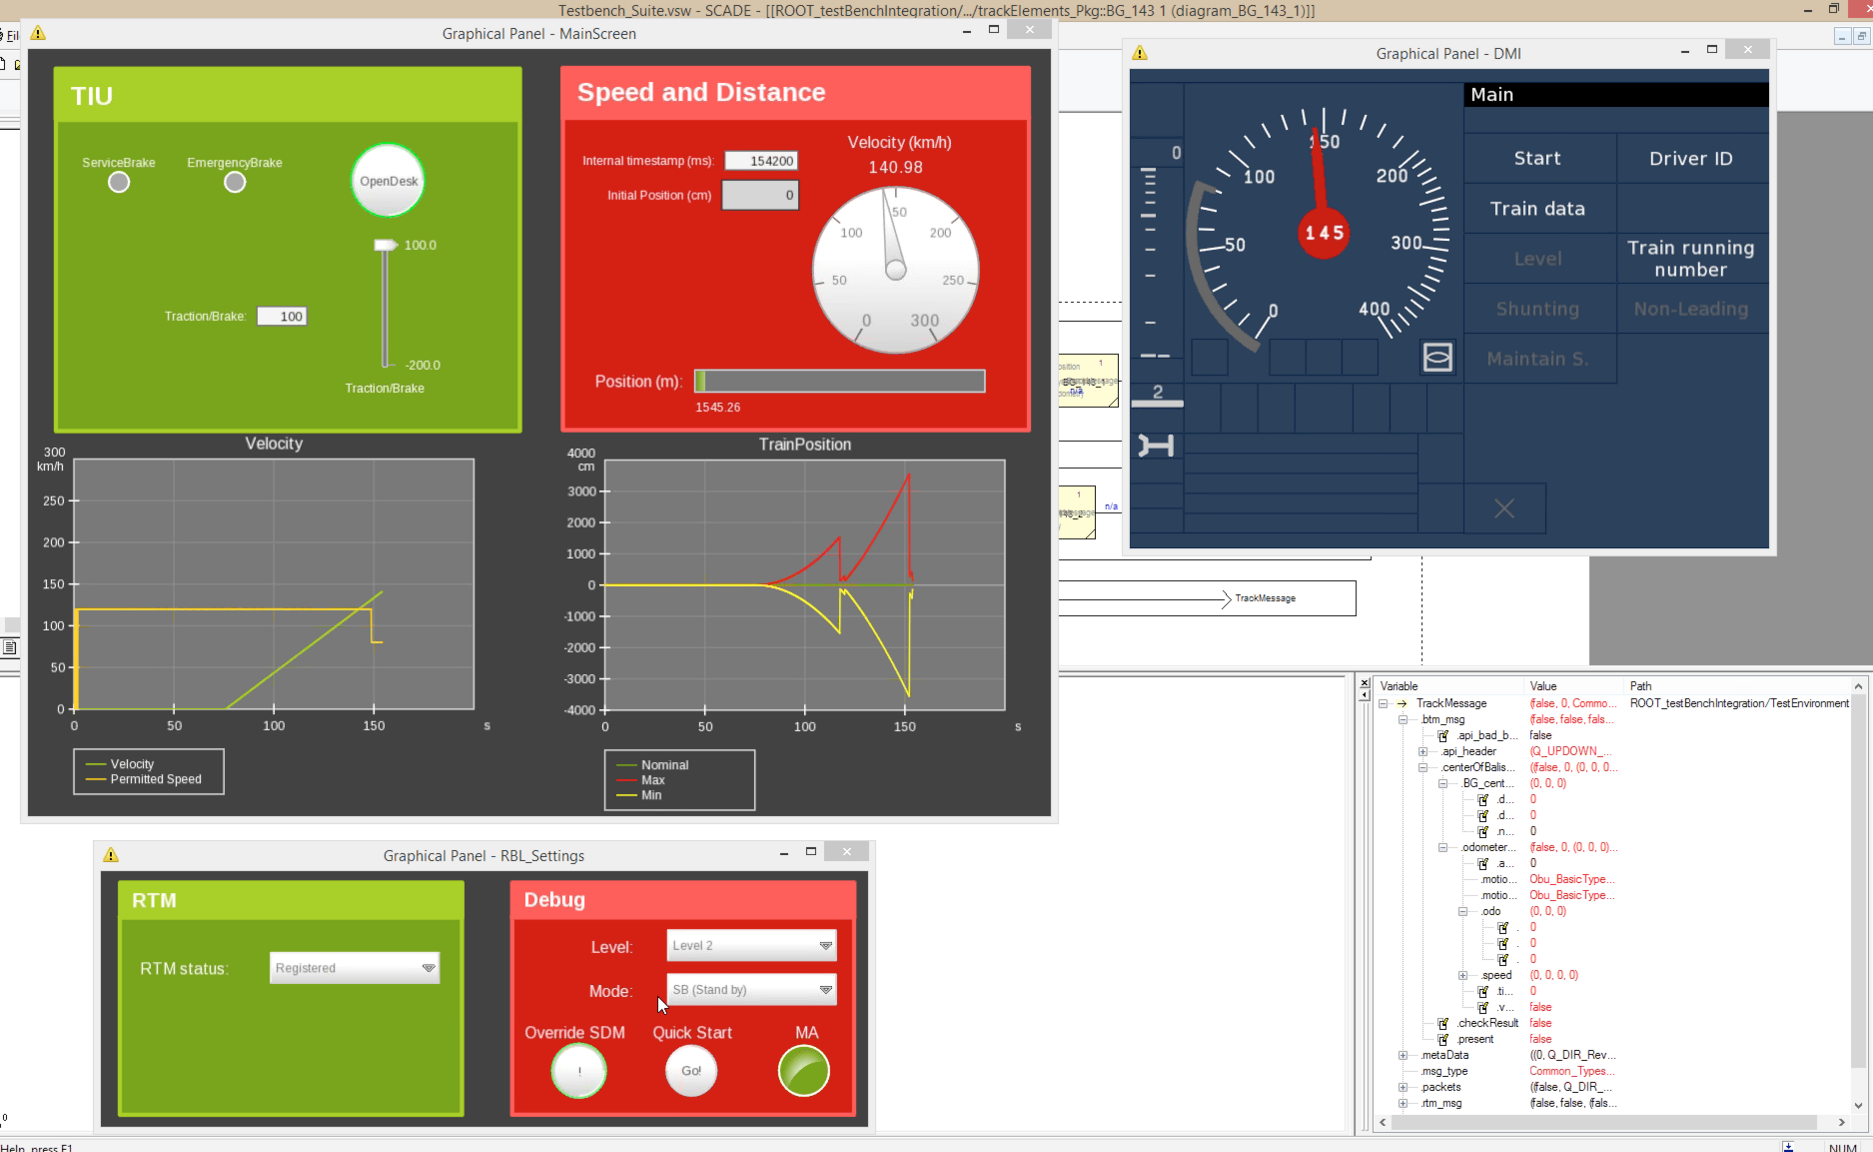
\includegraphics[width=\linewidth]{POC_environment.png}
  \caption{Environment for use case demonstration}
  \label{fig:WP3-demo}
\end{figure}




\section{Dynamic track model of the ETCS Level 2 line Amsterdam- Utrecht}

This environment model will be fourthly enhanced during the last project period, in order to:\\

•   Allow full dynamic simulation of the Utrecht- Amsterdam line\\
•   Form a basis for a (future) dynamic track simulator, which models the balise locations, balise messages and RBC messages for any given line, and which can automatically be generated from engineering datasets.\\
•   Provide a full track model for the purposes of openETCS\\
\\

(see Figure \ref{fig:track-dynamic}.)
	
\begin{figure}
  \centering
  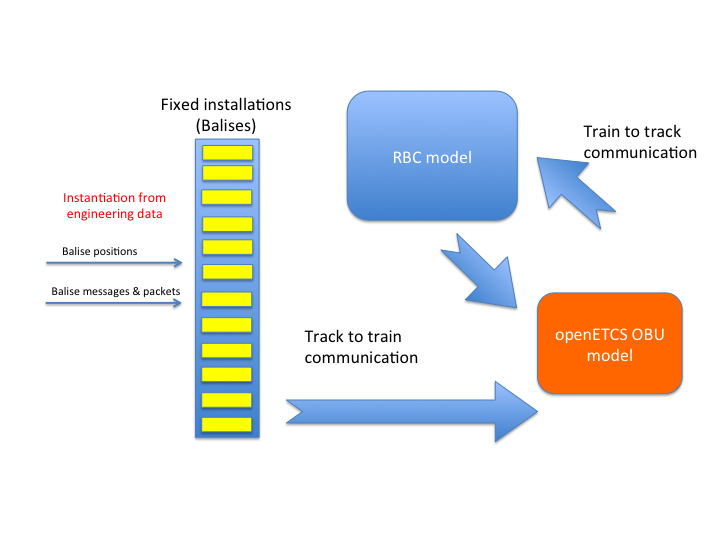
\includegraphics[width=\linewidth]{POC-track-dynamic.png}
  \caption{Schematic view of dynamic track model}
  \label{fig:track-dynamic}
\end{figure}

%
%
%
%





\chapter{Architecture Description}
%-----------------------------------------------------------------------
%\subsection{Mode and Level}
%-----------------------------------------------------------------------
%\tbc
%Baseliyos Jacob

\section{System Architecture view in ERA TSI Subset 25 Chapter 2 "Basic System Description"}
The system architecture is an outcome on the functional decomposition according to the analysis of the document in § 2 Input documents. A starting point for the first analysis is the System Strcuture in ERA TSI Subset 26 chapter 2 the subchapter 2.5 and 2.4.\\

Since we decided in the openETCS project not to consider all subsystem due to our using scope for the proof of concept on the ETCS Level 2 Utrecht - Amsterdam line, we analysed the necessary subsystem as seen here:\\

\subsection{System Structure from the subchapter 2.4. of ERA TSI Subset 26 chapter 2}

\begin{itemize}
\item 2.4.1.1	Due to the nature of the required functions, the ERTMS/ETCS system will have to be partly on the trackside and partly on board the trains. 
\item 2.4.1.2	This defines two sub-systems, the on-board sub-system and the trackside sub-system.
2.4.1.3	The environment of ERTMS/ETCS system is composed of:
\item a)	the train, which will then be considered in the train interface specification;
\item b)	the driver, which will then be considered via the driver interface specification;
\item c)	other onboard interfaces (see architecture drawing in 2.5.3),
\item d)	external trackside systems (interlockings, control centres, etc.), for which no 
\item interoperability requirement will be established.
\end{itemize}

\subsection{Sub System from the subchapter 2.5. of ERA TSI Subset 26 chapter 2}
\subsubsection{2.5.1 Trackside subsystem}
\paragraph{§ 2.5.1.1	Depending of the application level (see further sections), the trackside sub-system can be composed of:}
\begin{itemize}
\item a) balise
\item b) lineside electronic unit \textbf{\textit{- not in the scope of this project}}
\item c) the radio communication network (GSM-R)
\item d) the Radio Block Centre (RBC)
\item e) Euroloop \textbf{\textit{- not in the scope of this project}}
\item f) Radio infill unit \textbf{\textit{- not in the scope of this project}}
\item g) Key Management Centre (KMC) \textbf{\textit{- not in the scope of this project}}
\end{itemize}


\paragraph{2.5.1.2 Balise}
\begin{itemize}
\item 2.5.1.2.1	The balise is a transmission device that can send telegrams to the on-board sub-system.
\item 2.5.1.2.2	The balise is based on the existing Eurobalise specifications. These documents are included in the frame of the ERTMS/ETCS specifications.
\item 2.5.1.2.3	The balises provides the up-link, i. e. the possibility to send messages from trackside to the on-board sub-system.
\item 2.5.1.2.4	The balises can provide fixed messages or, when connected to a lineside electronic unit, messages that can be changed. 
\item 2.5.1.2.5	The balises will be organised in groups, each balise transmitting a telegram and the combination of all telegrams defining the message sent by the balise group.
\end{itemize}

\paragraph{2.5.1.3 Lineside electronic unit \textit{- not in the scope of this project}}
\begin{itemize}
\item 2.5.1.3.1	The lineside electronic units are electronic devices, that generate telegrams to be sent by balises, on basis of information received from external trackside systems.
\end{itemize}

\paragraph{2.5.1.4 Trackside radio communication network (GSM-R)}
\begin{itemize}
\item 2.5.1.4.1	The GSM-R radio communication network is used for the bi-directional exchange of messages between on-board sub-systems and RBC or radio infill units. 
\item 2.5.1.4.2	Intentionally deleted
\end{itemize}

\paragraph{2.5.1.5 RBC}
\begin{itemize}
\item 2.5.1.5.1	The RBC is a computer-based system that elaborates messages to be sent to the train on basis of information received from external trackside systems and on basis of information exchanged with the on-board sub-systems. 
\item 2.5.1.5.2	The main objective of these messages is to provide movement authorities to allow the safe movement of trains on the Railway infrastructure area under the responsibility of the RBC.
\item 2.5.1.5.3	The interoperability requirements for the RBC are mainly related to the data exchange between the RBC and the on-board sub-system.
\end{itemize}

\paragraph{2.5.1.6 Euroloop \textit{- not in the scope of this project}}
\begin{itemize}
\item 2.5.1.6.1	The Euroloop subsystem operates on Level 1 lines, providing signalling information in advance as regard to the next main signal in the train running direction.
\item 2.5.1.6.2	The Euroloop subsystem is composed of an on-board functionality and by one or more trackside parts. 
\end{itemize}
 
\paragraph{2.5.1.7 Radio infill Unit \textit{- not in the scope of this project}}
\begin{itemize}
\item 2.5.1.7.1	The RADIO INFILL subsystem operates on Level 1 lines, providing signalling information in advance as regard to the next main signal in the train running direction.
\item 2.5.1.7.2	The RADIO INFILL subsystem is composed of an on-board functionality and by one or more trackside parts (named RADIO INFILL Unit).
\end{itemize}
 
\paragraph{2.5.1.8 KMC \textit{- not in the scope of this project}}
\begin{itemize}
\item 2.5.1.8.1	The role of the KMC is to manage the cryptographic keys, which are used to secure the EURORADIO communications between the ERTMS/ETCS entities (ERTMS/ETCS on-board equipments, RBCs and RIUs).
\end{itemize}

\paragraph{2.5.2 On-board sub-system \textit{kernel part of the project}}

\textbf{2.5.2.1	Depending of the application level (see further sections), the on-board sub-system can be composed of:}
\begin{itemize}
\item a)	the ERTMS/ETCS on-board equipment;
\item b)	the on-board part of the GSM-R  radio system;
\end{itemize}


\textbf{2.5.2.2	ERTMS/ETCS on-board equipment}
\begin{itemize}
\item 2.5.2.2.1	The ERTMS/ETCS on-board equipment is a computer-based system that supervises the movement of the train to which it belongs, on basis of information exchanged with the trackside sub-system. 
\item 2.5.2.2.2	The interoperability requirements for the ERTMS/ETCS on-board equipment are related to the functionality and the data exchange between the trackside sub-systems and the on-board sub-system and to the functional data exchange between the on-board sub-system and:
\item a) the driver;
\item b) the train;
\item c) the onboard part of the existing national train control system(s).
\end{itemize}

\textbf{2.5.2.3	Onboard radio communication system (GSM-R)}
\begin{itemize}
\item 2.5.2.3.1	The GSM-R on-board radio system is used for the bi-directional exchange of messages between on-board sub-system and RBC or radio infill unit. 
\item 2.5.2.3.2	Intentionally deleted.
\end{itemize}

\paragraph{2.5.3. ERTMS/ETCS Reference Architecture}
\textit{\textbf{The figure below shows the system scope for design of the ETCS Subsystem regarding the openETCS Onboard Unit and the Test Environment within the scope of the openETCS project proof of conept on ETCS Level 2 Utrecht - Amsterdam.}}

\subsection{System Structure from the subchapter 2.4. of ERA TSI Subset 26 chapter 2}
\begin{figure}[h]
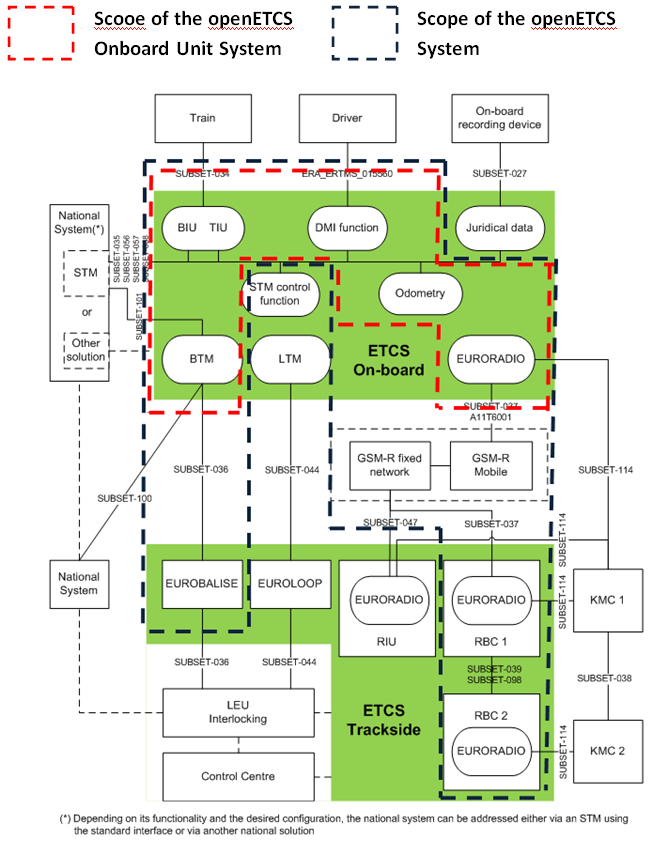
\includegraphics[scale=0.7]{images/ArchitectureSRS}
\caption{Scope of System according to ERA TSI Chapter 2}
\label{Scope of System according to ERA TSI Chapter 2}
\end{figure}

\section{System Architecture SysML View}
\textbf{The SysML System view of the architecture will reflect the scope accorgin to 4.1 and is a top down breakdown to the design layer. The functional breakdown has been done in Scade System and is part of the design model. Furthermore it will reflect all the external and internal interface that will will be described in 4.3. Another goal of the System Architecture SysML view is to explain and set the boundaries for the ETCS Kernel development "F2 Kernel" as the main design part of the openETCS@ITEA2 project.}

\subsection{1st level System Architecture view}
\textbf{All subystem of the ETCS/ERTMS Basic Sytem according in the scope of the openETCS@ITEA2 project will be reflected in this 1st level view. Furthermore the interlocking as part of a full Rail Signalling System, but not part of the openETCS scope, will be highlighted in this view.}

\textit{Interlocking =  interlocking is an arrangement of signal apparatus that prevents conflicting movements through an arrangement of tracks such as junctions or crossings. The signalling appliances and tracks are sometimes collectively referred to as an interlocking plant. An interlocking is designed so that it is impossible to display a signal to proceed unless the route to be used is proven safe.}


\begin{figure}[h]
\centering
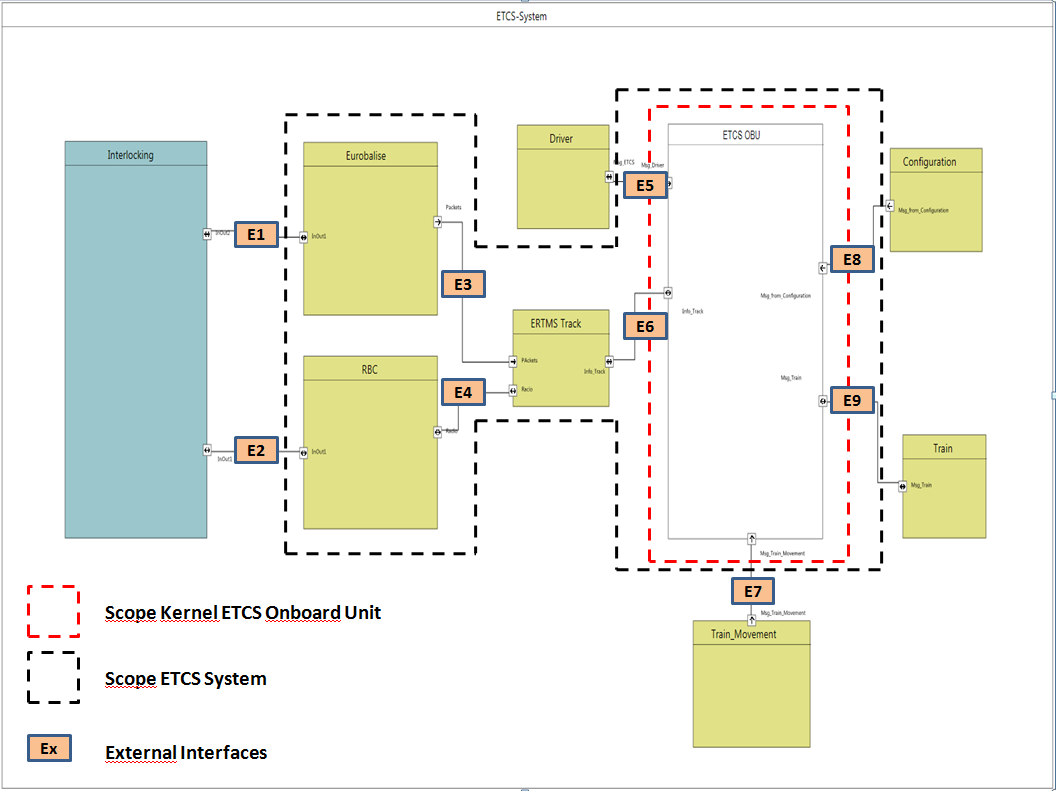
\includegraphics[scale=0.6]{images/1stlevelarchitecture}
\caption{1st level System Architecture view}
\label{1st level System Architecture view}
\end{figure}

\newpage
\subsection{2st level System Architecture view}
\textbf{The 2nd level system view will provide a decopmosition of the ETCS Onboard Unit systems and the Kernerl of the ETCS. The Kernel is the main part of the ETCS Onboard Unit system and reflects the functions specified in the ERA TSI Subset 26. Therefore the boundaries and interfaces to the other subasystems of the ETCS Onbard Unit needs to be fully desribed and formal. At least the formalisation kernel functions and boundaries should be realized in the openETCS project.}

\begin{figure}[h]
\centering
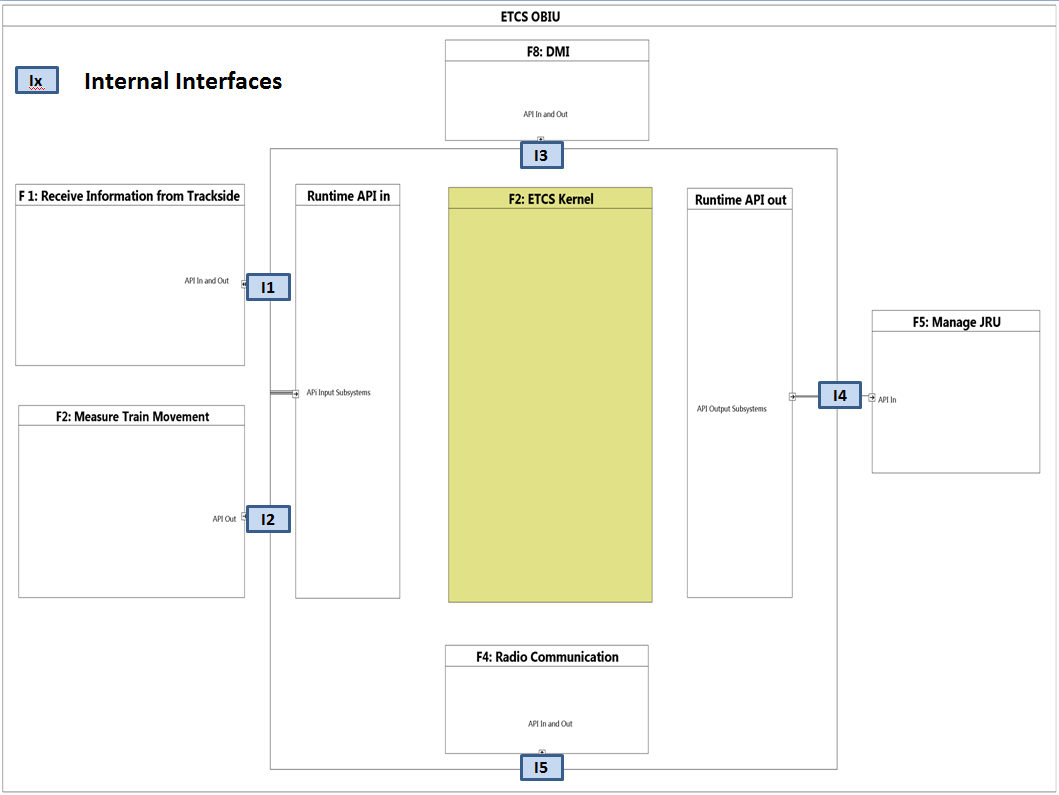
\includegraphics[scale=0.6]{images/2ndlevelarchitecture}
\caption{2nd level System Architecture view}
\label{2nd level System Architecture view}
\end{figure}

\subsection{3rd level System Architecture view}
\textbf{The 3rd level system view will provide a decopmosition of the ETCS Kernel of the ETCS Onboard Unit Systems. The decomposition and further design of the subfunctions of the kernel are part of the chapter 6 in this document. In chapter 6 we will consider the design description that will be completed by every designer itself. The designer can decided in this layer about the decomposition and boundaries of his subsystem, but need to describe the design choices.}

\newpage
\section{Interfaces}
\textbf{This section will consider the External and Internal interfaces as descibed in the system decomposition figures in 4.2.1 and 4.2.2}

\subsection{External Interfaces}
\textbf{External interfaces will describe the data flow between systems outside of the scope of the openETCS Project}

\paragraph*{E1: In- and Out flow between the Interlocking an Eurobalise. There will be 2 kind of balises}

\begin{itemize}
\item Fixed Balise: no interaction to the interlocking
\item Balise Controlled: interaction to the interlocking trough LEU
\end{itemize}

\begin{figure}[h]
\centering
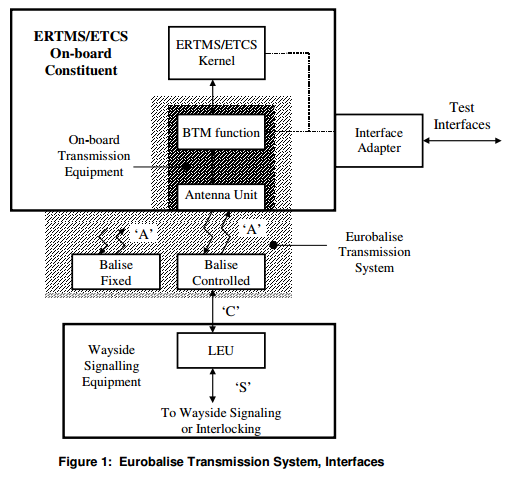
\includegraphics[scale=0.8]{images/Eurobalise}
\caption{Eurobalise}
\label{Eurobalise}
\end{figure}


\paragraph{E2: In- and Out flow between the Interlocking and Radio Block Control.}
This External interface will ensure the states or logics directly to the Radio Block Control and the other way back from the train to the interlocking.\\

\paragraph{E3:}

\paragraph{E4:}

\paragraph{E5:}

\paragraph{E6:}

\paragraph{E7:}

\paragraph{E8:}

\paragraph{E9:}

\subsection{Internal Interfaces}

\paragraph{I1:}

\paragraph{I2:}

\paragraph{I3:}

\paragraph{I4:}

\paragraph{I5:}



\chapter{Runtime API}

\section{Introduction to the Architecture}

\subsection{Abstract Hardware Architecture}

For proper understanding of openETCS API and of constraints imposed on
both sides of the API, we need to define a \emph{reference abstract hardware architecture}. This hardware architecture is ``abstract''
is the sense that the actual vendor specific hardware architecture
might be totally different of the abstract architecture described in
this chapter. For example, several units might be grouped together on
the same processor.

However, the actual vendor specific architecture shall fulfill all the
requirements and constraints of this reference abstract hardware
architecture and shall not request additional constraints.

\subsection{Definition of the Reference Abstract Hardware Architecture}

\begin{figure}
  \centering
  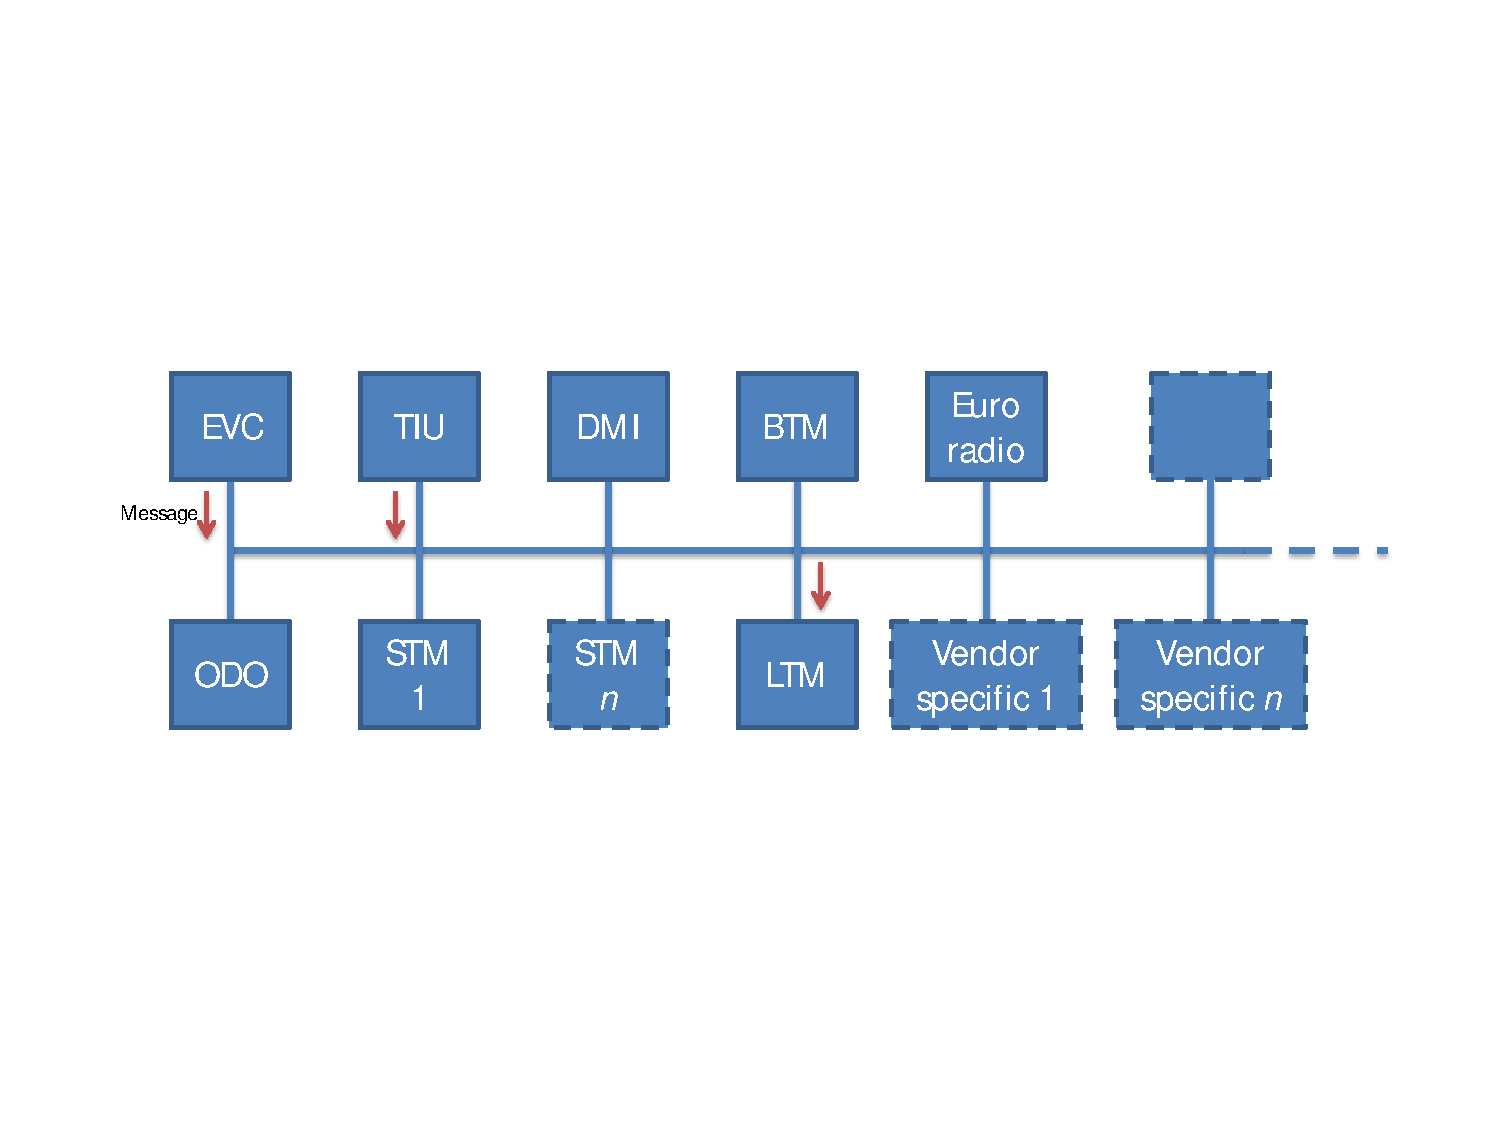
\includegraphics[width=\textwidth]{abstract-hardware-architecture.pdf}
  \caption{Reference abstract hardware architecture.}
  \label{fig:hardware-arch}
\end{figure}

The reference abstract hardware architecture is shown in Figure
\ref{fig:hardware-arch}. The reference abstract hardware architecture is made of a bus on which are connected \emph{units} defining the OBU:

\begin{itemize}
\item {EVC};
\item {TIU};
\item {ODO};
\item {DMI};
\item {STM};
\item {BTM};
\item {LTM}: Not part of this openETCS implementation;
\item EURORADIO;
\item {JRU}: Not part of this openETCS implementation;
\end{itemize}

Elements not being part of this implementation are marked. Those units shall working concurrently. They shall exchange information with other units through asynchronous message passing.

\subsection{Reference abstract software architecture}
\label{software-arch}

\begin{figure}
  \centering
  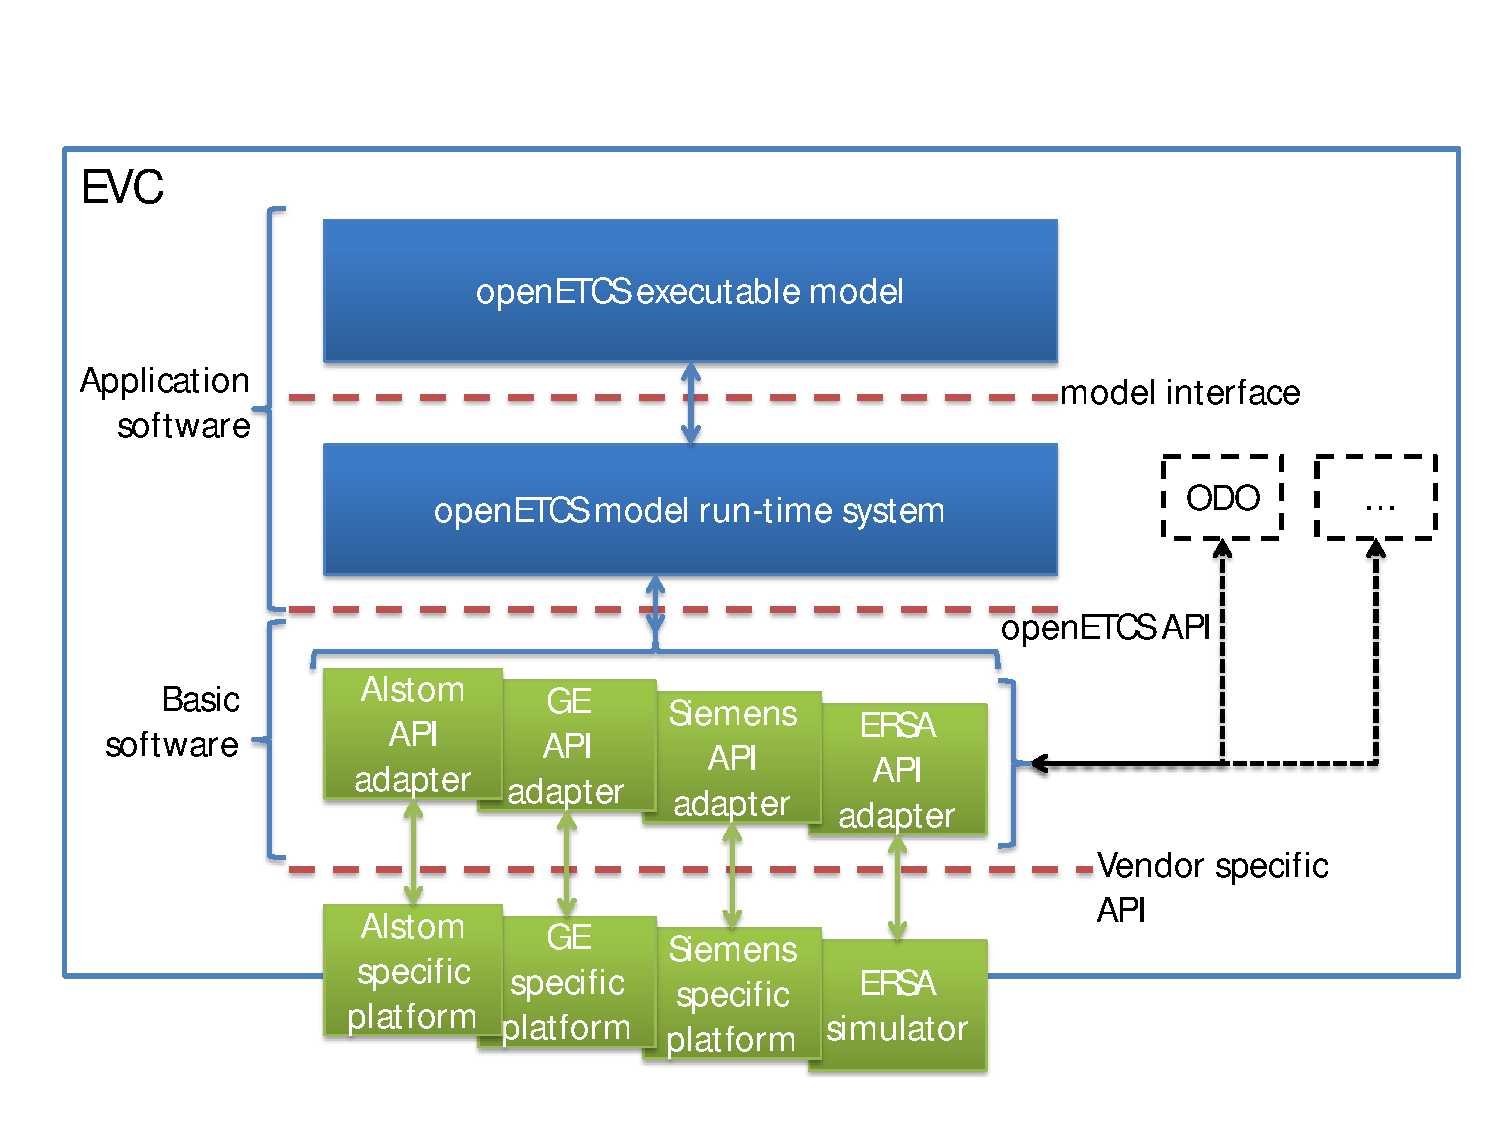
\includegraphics[width=0.9\textwidth]{software-architecture.pdf}
  \caption{Reference abstract software architecture}
  \label{fig:software-arch}
\end{figure}

The \emph{reference abstract software architecture} is shown in Figure
\ref{fig:software-arch}. This architecture consists of following
elements:
\begin{description}
\item[openETCS executable model] produced by the SCADE model \cite{scade-model}. It shall contain the program implementing core
  ETCS functions;
\item[openETCS model run-time system] shall help the execution
  of the openETCS executable model by providing additional functions
  like encode/decode messages, proper execution of the model through
  appropriate scheduling, re-order or prioritize messages, etc. 
\item[Vendor specific API adapter] shall make the link between
  the Vendor specific platform and the openETCS model run-time system.
  It can buffer message parts, encode/decode messages, route messages
  to other EVC components, etc.
\item[EVC] All above three elements shall be included in the EVC;
\item[Vendor specific platform] shall be all other elements of
  the system, bus and other units, as shown in Figure \ref{fig:hardware-arch}.
\end{description}

We have thus three interfaces:
\begin{description}
\item[Model interface]
 is the interface between openETCS executable model and openETCS model run-time system. 
\item[openETCS {API}]
 is the interface between openETCS model run-time system and Vendor specific {API} adapter.
\item[Vendor specific {API}]
 is the interface between Vendor specific {API} adapter and Vendor specific platform. This interface is not publicly described for all vendors. You can find the Alstom implementation as an example.
\end{description}

The two blocks openETCS executable model and openETCS model run-time
system are making the \emph{application software} part. This application software might be either openETCS reference software or vendor specific software.

The Vendor specific API adapter is making the \emph{Basic software} part.





\chapter{Design Description}

\section{F1: Receive information from Trackside}
\section{F2: ETCS Kernel}
%-----------------------------------------------------------------------
\subsection{Manage\_TrackSideInformation\_Integration}
%-----------------------------------------------------------------------
%\tbc
%Bernd Hekele

The block ``Manage\_TrackSideInformation\_Integration'' is responsible for receiving Eurobalise-telegrams and Euroradio-messages from the API and perform several consistency checks on the input.

The block collects the telegrams of balises in order to build balise group messages. Euroradio messages are always delivered as a whole message. 

On each message, a consistency check is performed, before the data is validated according to the driving direction of the train. In general, messages not designated for the current driving direction of the train are not forwarded to the further processing.

After applying consistency checks, the data direction is validated.

%Information of the odometer is used to control for the train leaving the expectation window of the balises. % TODO makes not much sense here.

\begin{figure}[H]
 \centering
 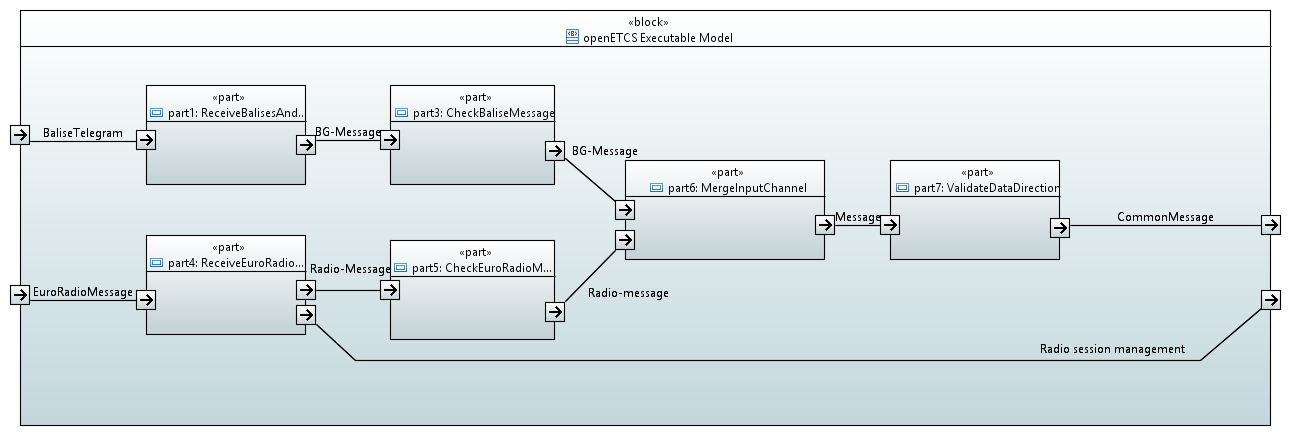
\includegraphics[width=\textwidth]{./images/Input-Messages4.PNG}
 % Input-Messages4.PNG: 0x0 pixel, 0dpi, nanxnan cm, bb=
 \caption{Structure of the Manage\_TrackSideInformation\_Integration module with submodules}
 \label{fig:receiveAndCheckConsistencyArch}
\end{figure}


\subsubsection{Input}
For providing the output, the module needs different input data flows. An overview is provided in table \ref{tbl:ReceiveMessageAndCheckConsistencyInput}

\begin{minipage}{\linewidth}
  \scriptsize
  \begin{tabular}{| c | l | l | l | l |}
    \hline
    \textbf{Index} & \textbf{Input name} & \textbf{Input type} & \textbf{Source}\\ \hline
    0 & \texttt{fullChecks} & \texttt{bool} & Configuration \\
    1 & \texttt{API\_trackSide\_Message} & \texttt{API\_Msg\_Pkg::API\_TrackSideInput\_T} & API\\
    2 & \texttt{ActualOdometry} & \texttt{Obu\_BasicTypes\_Pkg::odometry\_T} & Odometer\\
    3 & \texttt{reset} & \texttt{bool} & Environment\\
    4 & \texttt{trainPosition} & \texttt{TrainPosition\_Types\_Pck::trainPosition\_T} & Calculate Train Position\\
    5 & \texttt{modeAndLevel} & \texttt{BG\_Types\_Pkg::ModeAndLevelStatus\_T} & Mode and Level\\
    6 & \texttt{tNvContact} & \texttt{Obu\_BasicTypes\_Pkg::T\_internal\_Type} & Database\\
    7 & \texttt{lastRelevantEventTimestamp} & \texttt{Obu\_BasicTypes\_Pkg::T\_internal\_Type} & Database\\
    8 & \texttt{connectionStatus} & \texttt{Radio\_Types\_Pkg::sessionStatus\_Type} & Manage Radio Communication\\
    9 & \texttt{inSupervisingRbcId} & \texttt{int} & Database\\
    10 & \texttt{inAnnouncedBGs} & \texttt{TrainPosition\_Types\_Pck::positionedBGs\_T} & Calculate Train Position\\
    11 & \texttt{q\_nvlocacc} & \texttt{Q\_NVLOCACC} & Database\\
    \hline
  \end{tabular} 
  \captionof{table}{Overview over input}
  \label{tbl:ReceiveMessageAndCheckConsistencyInput}
\end{minipage}

\paragraph{Input 0: \texttt{fullChecks\\}}
The boolean indicates, if all checks on the message should be performed. The possible values are given in table \ref{tbl:fullChecks}.

\begin{minipage}{\linewidth}
 \begin{tabular}{| l | p{9cm} |}
    \hline
    \textbf{Value} & \textbf{Interpretation}\\ \hline
    true & All checks are performed.\\
    false & The module \texttt{Information Filter} is deactivated.\\
    \hline
  \end{tabular} 
  \captionof{table}{Possible values for the input \texttt{fullChecks}}
  \label{tbl:fullChecks}
\end{minipage}

\paragraph{Input 1: \texttt{API\_trackSide\_Message}}

The \texttt{API\_trackSide\_Message} is the message received from the API. The API performs preprocessing of RTM and BTM messages and deliveres a maximum of a single message per cycle to the SCADE model.

\paragraph{Input 2: \texttt{ActualOdometry}}
The input \texttt{ActualOdometry} is provided by the external odometry module of the train. It contains location information with inaccuracies.

\paragraph{Input 3: \texttt{reset}\\}
To delete all data stored in the module (e.g. collected balise-telegrams, which do not yet form a complete message), a reset input can be used. If the input is set to \texttt{true}, all data kept in the module is deleted and no input is accepted.

\begin{minipage}{\linewidth}
   \begin{tabular}{| l | p{9cm} |}
    \hline
    \textbf{Value} & \textbf{Interpretation}\\ \hline
    true & All data kept in the module is deleted and no input is accepted.\\
    false & No action. Data at input is accepted.\\
    \hline
  \end{tabular} 
  \captionof{table}{Possible values for the input \texttt{reset}}
  \label{tbl:reset}
\end{minipage}


\paragraph{Input 4: \texttt{trainPosition}}
The input \texttt{trainPosition} is generated by the ``Calculate Train Position'' module and contains the current position of the train.

\paragraph{Input 5: \texttt{modeAndLevel}}
The input is generated by the ``Mode and level management'' module. It provides the current level and mode of the EVC.

\paragraph{Input 6: \texttt{tNvContact}}

For monitoring the safe radio connection, the national value \texttt{T\_NVCONTACT} is needed as an input.

\paragraph{Input 7: \texttt{lastRelevantEventTimestamp}}

For monitoring the safe radio connection, it's necessary, that the time between two packets is less than the value of \texttt{T\_NVCONTACT}.

In situations like level-changes or announced radioholes, not the timestamp of the last message is relevant for comparison, but the timestamp of the last relevant event. This can be e.g. the timestamp of the level change or the timestamp of the timestamp of the moment, when the train was passing the end of the radiohole. 

For performing this check, the timestamp of the last relevant event is provided to the model as an \texttt{T\_internal\_Type}-type.

\paragraph{Input 8: \texttt{connectionStatus}\\}
The input \texttt{connectionStatus} will give information about the radio connection. This input is delivered by the session management module, not from the API. The information is needed to perform the timing check, which is depending on the connection state.

\begin{minipage}{\linewidth}
  \begin{tabular}{| l | p{9cm} |}
    \hline
    \textbf{Value} & \textbf{Interpretation}\\ \hline
    DISCONNECTED & The OBU is currently not connected to a RBC.\\
    CONNECTING & The OBU is currently connecting to the RBC. Received messages belong to the process of establishing a connection.\\
    CONNECTION\_ESTABLISHED &  The connection to RBC is established.\\
    \hline
  \end{tabular} 
  \captionof{table}{Possible values for the input \texttt{connectionStatus}}
  \label{tbl:connectionStatus}
\end{minipage}

\paragraph{Input 9: \texttt{inSupervisingRbcId}}
For the submodule ``Information Filter'', the information is needed, which radio messages are sent by the supervising RBC. To recognize these messages, the identifier of the supervising RBC is needed.

\paragraph{Input 10: \texttt{inAnnouncedBGs}}
This input provides information about balise groups which will be passed by the train soon. This information is generated by ``Calculate Train Position'' based on the linking information received from trackside.

\paragraph{Input 11: \texttt{q\_nvlocacc}}
The national value determines the location accuracy and is delivered by the database.



\subsubsection{Output}
The output of the module provides the received and processed Euroradio and Eurobalise messages. The module combines messages both from Eurobalises and from Euroradio to one common dataflow.

An overview over the output dataflows is provided in table \ref{tbl:ReceiveMessageAndCheckConsistencyOutput}.

\begin{minipage}{\linewidth}
 \footnotesize
  \begin{tabular}{| c | l | l | l |}
    \hline
    \textbf{Index} & \textbf{Output name} & \textbf{Output type}\\ \hline
    0 & \texttt{outputMessage} & \texttt{Common\_Types\_Pkg::ReceivedMessage\_T}\\
    1 & \texttt{ApplyServiceBrake} & \texttt{bool}\\
    2 & \texttt{BadBAliseMessageToDMI} & \texttt{bool}\\
    3 & \texttt{errorLinkedBG} & \texttt{bool}\\
    4 & \texttt{errorUnlinkedBG} & \texttt{bool}\\
    5 & \texttt{passedBG} & \texttt{BG\_Types\_Pkg::passedBG\_T} \\
    6 & \texttt{outPositionParams} & \texttt{Common\_Types\_Pkg::PositionReportParameter\_T} \\
    7 & \texttt{outRadioManagement} & \texttt{Common\_Types\_Pkg::radioManagementMessage\_T} \\
    8 & \texttt{radioSequenceError} & \texttt{bool} \\
    9 & \texttt{radioMessageConsistencyError} & \texttt{bool} \\
    \hline
  \end{tabular} 
  \captionof{table}{Dataflow at output}
  \label{tbl:ReceiveMessageAndCheckConsistencyOutput}
\end{minipage}

\subparagraph{Output 0: \texttt{outputMessage}\\}
The element \texttt{outputMessage} consists of the type \texttt{ReceivedMessage\_T} combines both balise and radio messages to one common datatype. This datatype contains all variables and packets, which are possible for the given scenario.

\begin{minipage}{\linewidth}
  \scriptsize
  \begin{tabular}{| l | l | p{5.5cm} |}
  \hline
  \textbf{Name} & \textbf{Datatype} & \textbf{Description}\\ \hline
  \texttt{valid} & \texttt{bool} & true, if no consistency errors were detected.\\
  \texttt{source} & \texttt{Common\_Types\_Pkg::MsgSource\_T} & Defines, if this is a Euroradio or Eurobalise message.\\
  \texttt{packetMetadata} & \texttt{Common\_Types\_Pkg::Metadata\_T} & contains the metadata of the packets\\
  \texttt{radioMetadata} & \texttt{Common\_Types\_Pkg::RadioMetadata\_T} & contains the metadata of the radio specific header variables\\
  \texttt{BG\_Common\_Header} & \texttt{BG\_Types\_Pkg::BG\_Header\_T} & Header of Eurobalise message\\
  \texttt{Radio\_Common\_Header} & \texttt{Radio\_Types\_Pkg::Radio\_TrackTrain\_Header\_T} & Header of Euroradio message\\
  \texttt{packets} & Common\_Types\_Pkg::Packets\_T & Structure of packets in messages\\
  \hline
\end{tabular}
  \captionof{table}{Structure of \texttt{ReceivedMessage\_T}}
  \label{tbl:receivedMessage_structure}
\end{minipage}


The Eurobalise-common-header \texttt{BG\_Header\_T} consists of the fields visible in the SCADE-declaration. The structure corresponds to the structure defined in the SRS chapter 8.4.2.1. Some fields were removed since they are not needed anymore for further processing after building messages from separate telegrams.

The Euroradio-common-header \texttt{Radio\_TrackTrain\_Header\_T} consists of the fields visible in the SCADE declaration. The structure corresponds to the structure defined in the SRS chapter 8.4.4.6.1. The structure contains all variables required by possible \texttt{NID\_MESSAGE} values for the given scenario. Which values are valid is defined in the field \texttt{radioMetadata}.

%\textbf{TODO:} Different definition of Radio-header than in SCADE!

%\textbf{TODO:} Note on packet type definitions and implementation details (which values were not used).

%\textbf{Note:} Packet 44 not used (applications outside the ERTMS/ETCS system are not supported by this implementation).

%\textbf{TODO:} Define packets 136, 12 in SCADE.

\subparagraph{Output 1: \texttt{ApplyServiceBreak}}
The flag indicates the balise group the train just passed could not be processed correctly. The check results in the request for a service break.

\subparagraph{Output 2: \texttt{BadBaliseMessageToDMI}}
Information to be passed to the DMI to indicate the reception of a ``bad balise'' to the driver.

\subparagraph{Output 3: \texttt{errorLinkedBG}\\}

\begin{minipage}{\linewidth}
  \begin{tabular}{| l | p{9cm} |}
    \hline
    \textbf{Value} & \textbf{Interpretation}\\ \hline
    true & A error in a linked balise group was detected.\\
    false & No error in a linked balise group was detected.\\
    \hline
  \end{tabular} 
  \captionof{table}{Possible values for the input \texttt{errorLinkedBG}}
  \label{tbl:errorLinkedBG}
\end{minipage}

\subparagraph{Output 4: \texttt{errorUnlinkedBG}\\}
\begin{minipage}{\linewidth}
  \begin{tabular}{| l | p{9cm} |}
    \hline
    \textbf{Value} & \textbf{Interpretation}\\ \hline
    true & A error in an unlinked balise group was detected.\\
    false & No error in an unlinked balise group was detected.\\
    \hline
  \end{tabular} 
  \captionof{table}{Possible values for the input \texttt{errorUnlinkedBG}}
  \label{tbl:errorUnlinkedBG}
\end{minipage}

\subparagraph{Output 5: \texttt{passedBG}}
The output \texttt{passedBG} provides the received balise group message in a special format needed by the module ``Calculate train position''.

\subparagraph{Output 6: \texttt{outPositionParams}}
The output \texttt{outPositionParams} provides the parameters for the position report in a special format needed by the module ``Provide Position Report''.

\subparagraph{Output 7: \texttt{outRadioManagement}}
The output \texttt{outRadioManagement} provides the messages for radio session management in a special format needed by the module ``Management of Radio Communication''.

\subparagraph{Output 8: \texttt{radioSequenceError\\}}

\begin{minipage}{\linewidth}
  \begin{tabular}{| l | p{9cm} |}
    \hline
    \textbf{Value} & \textbf{Interpretation}\\ \hline
    true & A sequence error or a timeout has been detected in the radio message.\\
    false & No error in the radio message sequence was detected.\\
    \hline
  \end{tabular} 
  \captionof{table}{Possible values for the input \texttt{radioSequenceError}}
  \label{tbl:radioSequenceError}
\end{minipage}

\subparagraph{Output 9: \texttt{radioMessageConsistencyError\\}}

\begin{minipage}{\linewidth}
  \begin{tabular}{| l | p{9cm} |}
    \hline
    \textbf{Value} & \textbf{Interpretation}\\ \hline
    true & A consistency error has been detected in the radio message.\\
    false & No consistency error in the radio message was detected.\\
    \hline
  \end{tabular} 
  \captionof{table}{Possible values for the input \texttt{radioMessageConsistencyError}}
  \label{tbl:radioMessageConsistencyError}
\end{minipage} 

~\\

\subsubsection{Receive\_TrackSide\_Msg in Manage\_TrackSideInformation\_Integration}

\paragraph{Reference to the SRS (or other requirements)}
\begin{itemize}
  \item \cite[Chapt.~7 and 8]{subset-026}: Definition of the Balise Telegram
  \item \cite[Chapt.~4.2.2, 4.2.4, 4.2.9]{subset-036}: Interface to the BTM
  \item \cite[Chapt.~3.4.1 - 3.4.3, 3.16.2]{subset-026}: Handling of Balise Telegrams
  \item \cite[Chapt.~3.16.2]{subset-026}: Check of the balise group
  \item \cite[Chapt.~3.4.2]{subset-026}: Determining the orientation
  \item \cite[Chapt.~4.5.2]{subset-026}: Active Functions Table
  \item \cite[Chapt.~8.4.4]{subset-026}: Rules for Euroradio messages

\end{itemize}
\paragraph{Short description of the functionality}
This function defines the interface of the OBU model to the openETCS generic API for Eurobalise  and Euroradio messages. On the interface, either a valid telegram/message is provided or a telegram/message is indicated which could not be received correct when passing the balise or receiving the radio message. The function passes a balise telegram without major changes of the information to the next entity for collecting the balise group information. This entity collects telegrams received via the interface into Balise Group Information. In case of a radio message, the message is converted to an internal format for further processing and passed without changing the information contained.

\paragraph{Interface}
\paragraph{Functional Design Description}
\textbf{Design Constraints and Choices}
\begin{enumerate}
\item The decoding of balises is done at the API. Also, packets received via the interface are already transformed into a usable shape.
\item Only packets used inside the current model are passed via the interface.\\
\item Treatment of Packet 5: Linking Information.\\
Linking Information is added to the linking array starting from index 0 without gaps. Used elements are marked as valid. Elements are sorted according to the order given by the telegram sequence.
\item Telegrams received as invalid are passed to the ``Check-Function'' to process errors in communication with the track side according to the requirements and in a single place.
Telegrams are added to the telegram array starting from index 0 without gaps. Used elements are marked as valid. Elements are stored according to the order given by the telegram sequence.
\item This function does not process information from the packets. The information is passed to the check without further processing of the values. 
\end{enumerate}
\paragraph{Reference to the Scade Model}
The SCADE model can be found on github under the following path:

\tiny\url{https://github.com/openETCS/modeling/tree/master/model/Scade/System/ObuFunctions/ManageLocationRelatedInformation/BaliseGroup/Receive_TrackSide_Msg}
\normalsize
\subsubsection{CheckBGConsistency in Manage\_TrackSideInformation\_Integration}%Mainfunction receive track data. Name should be be defined and substituded by the designer of the function. 
\paragraph{Reference to the SRS or other Requirements (or other requirements)}
\begin{itemize}
  \item \cite[Chapt.~7 and 8]{subset-026}: Definition of the Balise Telegram
  \item \cite[Chapt.~3.4.1 - 3.4.3, 3.16.2]{subset-026}: Handling of Balise Telegrams
  \item \cite[Chapt.~3.16.2]{subset-026}: Check of the balise group
  \item \cite[Chapt.~4.5.2]{subset-026}: Active Functions Table
\end{itemize}
\paragraph{Short description of the functionality}
This function has the task  to verify the completeness and correctness of the received messages from balise groups.\\
A message consists of at least a telegram and a maximum of 8 telegrams.\\

\begin{itemize}
\item A message is still complete and correct, if a telegram is missing (or not decoded or incomplete decoded ), and this telegram is duplicated within the balise group and the duplicating one is correctly read.
\item By more than one telegram, the order of the telegrams must be either ascending (nominal) or descending(reverse).\\
\item A message is correct, if  all message counters (M MCUNT) do not equal 254 (that means: The telegram never fits any message of the group).\\ A message counter can be equal 255 (that means: The telegram fits with all telegrams of the same balise group) and all other values must be the same.\\
\end{itemize}

\paragraph{Interface}
An input of the operator is a list of recived telegrams. \\
After consistency check of the telegrams' list, the function generates the balise-group-message.\\
This function is active in certain modes and the output and reactions are dependent on if the linking information is used.\\

\paragraph{Functional Design Description}
The orientation of the BG will also be calculated in this block.\\
The check, if the message has been received in due time and the right at the right expected location, will be performed in "Calculate Train Position".\\
The checks on the validity of the data in the packets and the validity with respect to the direction of motion will be performed in other modules, e.g. "Validate Data Direction" .

\paragraph{Reference to the Scade Model}
The SCADE model can be found on github under the following path:

\tiny\url{https://github.com/openETCS/modeling/tree/master/model/Scade/System/ObuFunctions/ManageLocationRelatedInformation/BaliseGroup/CheckBGConsistency}
\normalsize

\subsubsection{CheckEuroradioMessage in Manage\_TrackSideInformation\_Integration}%Mainfunction receive track data. Name should be be defined and substituded by the designer of the function. 
\paragraph{Reference to the SRS or other Requirements (or other requirements)}
\begin{itemize}
 \item \cite[Chapt.~8.4.4]{subset-026}: Rules for Euroradio messages
 \item \cite[Chapt.~3.16]{subset-026}: Data consistency
\end{itemize}
\paragraph{Short description of the functionality}

The operator ``CheckEuroradioMessage'' performs several checks on the received radio message. These checks include checking of the message sequence, completeness of messages. Invalid messages are marked as invalid in the message header.

\paragraph{Interface}
The operator expects a radio message, information about the timestamp of the last relevant event, the national value for timeout (\texttt{T\_NVCONTACT}) and the status of the radio connection as input. The operator provides as output the radio message marked as valid or invalid in the message header and updated metadata in the message. Errors are indicated through boolean outputs.

\paragraph{Functional Design Description}

The operator performs the following checks:
\begin{itemize}
 \item Content checks
 \begin{itemize}
    %\item The computed length of the message must be equal to the value in \texttt{L\_MESSAGE}. (SRS 8.4.4.2.1)
    \item The whole message must be complete and contains all necessary fields. \cite[3.16.1.1]{subset-026}
    \item The message must respect the ETCS language. \cite[3.16.1.1]{subset-026} The operator checks, if all necessary variables and packets for the corresponding message are part of the message and if no packets and variables are included in the message, which are not allowed.
    %\item The variables of the message do not contain invalid values. \cite[3.16.1.1]{subset-026} % already done by API?
    %\item Check if the specified priority of message is equal to the priority with which the message was received. \cite[3.16.3.1.3.1]{subset-026}
  \end{itemize}
  \item Timing checks
  \begin{itemize}
    \item Check if the timestamp of a message is greater than the timestamp of the message received before. \cite[3.16.3.3.3]{subset-026}
    \item If a message contains the timestamp ``Unknown'', check if this message is part of the initiation of the communication session. \cite[3.16.3.3.4]{subset-026}
    \item Perform the check with the current message $n$:  $T\_TRAIN_{n} <= T\_TRAIN_{n-1} + T\_NVCONTACT$ \cite[3.16.1.1]{subset-026}. This ensures, that the message was received in due time.
  \end{itemize}
\end{itemize}

For inconsistent messages, the following actions are performed by the operator:

\begin{itemize}
  \item If a message is not consistent, it shall be rejected. \cite[3.16.3.1.1.1]{subset-026} For this purpose, the message is marked as invalid, so it can be rejected by the operators using the output of the CheckEuroradioMessage-operator.
  \item The RBC shall be informed, when a message was rejected. \cite[3.16.3.1.1.2]{subset-026} Therefore the necessary information for creating an error report is provided as boolean flags. 
  %\item If the RBC requested an ACK for a received message, message will be marked for the module to send a report to the RBC. (SRS 3.16.3.5)
  \item This operator will not trigger the reaction for an interrupted radio connection to the RBC. The reaction sepcified by \texttt{M\_NVCONTACT} will be triggered by the RBC session management module.
\end{itemize}

The check by the Euroradio-protocol \cite[3.16.3.1.1]{subset-026} will not be performed by the operator, but on a lower level (RTM or openETCS-API).

The operator is not responsible for checking the integrity of the message in the bitstream format. The bitwalker, which is converting the bitstream into the internally used datatypes, is performing the checks, which are only possible on the raw data. This includes a CRC check on the whole message and a value range check for each variable. If a consistency error is detected by the bitwalker, it is signalled to the model. If the bitwalker marks a packet as valid, all variables are expected to contain a valid value. The bitwalker is not part of the ETCS kernel.

Safe connection supervision is not in the scope of this operator. This functionality will be implemented by the ``Management of Radio communication'' module.

\paragraph{Reference to the Scade Model}
The SCADE model can be found on github under the following path:

\tiny\url{https://github.com/openETCS/modeling/tree/master/model/Scade/System/ObuFunctions/ManageLocationRelatedInformation/BaliseGroup/CheckEuroRadioMessage}
\normalsize

\subsubsection{ValidateDataDirection in Manage\_TrackSideInformation\_Integration}

\paragraph{Reference to the SRS or other Requirements (or other requirements)}
\begin{itemize}
 \item The functionality is mainly described in \cite[Chapter~3.6.3]{subset-026}.
\end{itemize}
\paragraph{Short description of the functionality}
The operator will filter an input message in order to mark all elements as invalid, which are not designated for the current driving direction of the train.

\paragraph{Interface}
The operator expects a message and information about the LRBG, passed balises and the current train position. As output, the message with packets valid for the current direction of driving is provided.
\paragraph{Functional Design Description}
\begin{itemize}
 \item The operator contains two processing paths for different message types. Radio messages and balise group messages are handeled in a different way. For validating the data direction of a radio message, the check is performed using the balise group referenced in the radio message header as relevant balise group. For balise group message, the LRBG is used.
 \item The metadata of packets, which are recognized as not valid for the current driving direction, is invalidated.
\end{itemize}

\paragraph{Reference to the Scade Model}
The SCADE model can be found on github under the following path:

\tiny\url{https://github.com/openETCS/modeling/tree/master/model/Scade/System/ObuFunctions/ManageLocationRelatedInformation/BaliseGroup/ValidateDataDirection}
\normalsize

\subsubsection{InformationFilter}

\paragraph{Reference to the SRS and other requirements}
\begin{itemize}
 \item The functionality of the InformationFilter is described in \cite[Chapter~4.8]{subset-026}.
\end{itemize}

\paragraph{Short description of the functionality}
The function InformationFilter filters incoming information received
from Eurobalise, Euroradio, and Euroloop. The information is received
via messages and filtering is done depending on the criteria described
in \cite[Chapter~4.8]{subset-026}. Messages are only allowed to pass
the filter if specified critera are met like for example the correct
mode of the train (e.g. Full Supervision, Shunting, etc.) or the ETCS
level. Some messages have to be stored in a TransitionBuffer to be
later reevaluated by the filter again.

\paragraph{Interface}
The interface of the information filter contains mainly the incoming
message and inputs to check for the conditions described in the
SRS. The complete interface is shown in table \ref{tbl:InformationFilterInterface}.

\begin{minipage}{\linewidth}
  \scriptsize
  \begin{tabular}{| l | l | l |}
    \hline
    \textbf{Name}                    & \textbf{Direction} & \textbf{Description}                                        \\ 
    \hline
    \texttt{inMessage}               & \texttt{IN}        & Received message that is valid for the train direction      \\
    \texttt{inLevel}                 & \texttt{IN}        & The current ETCS Level                                      \\
    \texttt{inMode}                  & \texttt{IN}        & The current train mode                                      \\
    \texttt{inSupervisingDevice}     & \texttt{IN}        & The device id which communicates with the current supervising
  RBC                                                                                                                   \\
    \texttt{inPendingL1Transition}   & \texttt{IN}        & Information if an ETCS Level 1 transition is pending        \\
    \texttt{inPendingL1L2Transition} & \texttt{IN}        & Information if an ETCS Level 2/3 transition is pending      \\
    \texttt{inPendingNTCTransition}  & \texttt{IN}        & Information if a NTC transition is pending                  \\
    \texttt{inPendingAckOfTrainData} & \texttt{IN}        & Information if the acknowledgement of train data is pending \\
    \texttt{inEmergencyBrakeActive}  & \texttt{IN}        & Information if the emergency brake is active                \\
    \texttt{inLastAckTextMessageId}  & \texttt{IN}        & The id of the last acknowledged message ID                  \\
    \texttt{inActiveCab}             & \texttt{IN}        & Information if the cab is active                            \\
    \texttt{inTrainDataValid}        & \texttt{IN}        & Information if the train data is valid                      \\
    \texttt{outMessage}              & \texttt{OUT}       & The filtered input message                                  \\
    \hline
  \end{tabular}
  \captionof{table}{Overview of the InformationFilter interface}
  \label{tbl:InformationFilterInterface}
\end{minipage}

\paragraph{Functional Design Description}

\begin{figure}[hbtp]
\centering
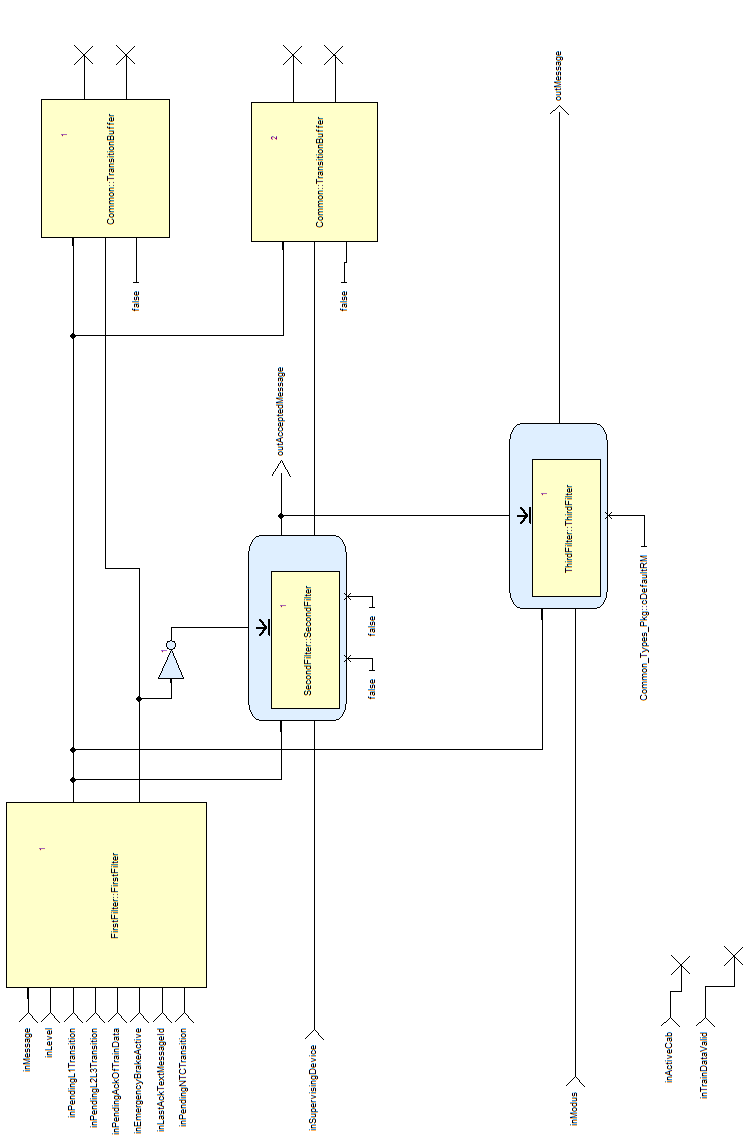
\includegraphics [scale=0.8]{images/informationfilter-high-level-rot.png}
\caption{High level overview of the InformationFilter components.}
\label{fig:InformationFilterHighLevel}
\end{figure}

The filter receives track information (balise and radio) and filter
them depending of the mode, level and further information. Only
messages that pass the filter are valid and should be considered by
other ETCS subsystems. The figure \ref{fig:InformationFilterHighLevel}
show the high\-level decomposition of the functionality. The filter
functionality can be decomposed into a FirstFilter, SecondFilter,
ThirdFilter an TransitionBuffer.

\paragraph{FirstFilter} This filter performs filtering of messages
based on the current ETCS level. The decisions taken process is
described via a big decision table which contains rows for every
packet and columns for every ETCS level. This table encodes also if
certain additional information is necessary to filter a message like
pending ETCS Level transitions. Based on this filter packets of an
incoming message is either rejected, accepted or the whole message is
put in the TransitionBuffer. Messages are put in the TransitionBuffer
if there is an announced level transition and the received message is
only valid for the upcoming level.

\paragraph{SecondFilter} The SecondFilter mainly considers messages
that are received via Euroradio. Certain messages are directly
rejected while other may be stored in the TransitionBuffer. The buffer
is used to store messages that are received from non supervising RBCs,
but will be reevaluated after a RBC transition.

\paragraph{ThirdFilter} The last filter is functionally very similiar
the the FirstFilter, however it filters depending on the mode. It also
contains a decision table with rows for every packet but the columns
are modes.

\paragraph{TransitionBuffer} The InformationFilter uses two
TransitionBuffers. One is used to store up to three messages for the
ETCS level transition and the other buffer is used for RBC
transitions. The buffer is designed as a ring buffer and message are
read in FIFO order.

A detailed list of packages and their handling depending of ETCS level
or mode can be seen in table \ref{fig:PackagesListLevel} and
\ref{fig:PackagesListMode}.

\begin{figure}[hbtp]
\centering
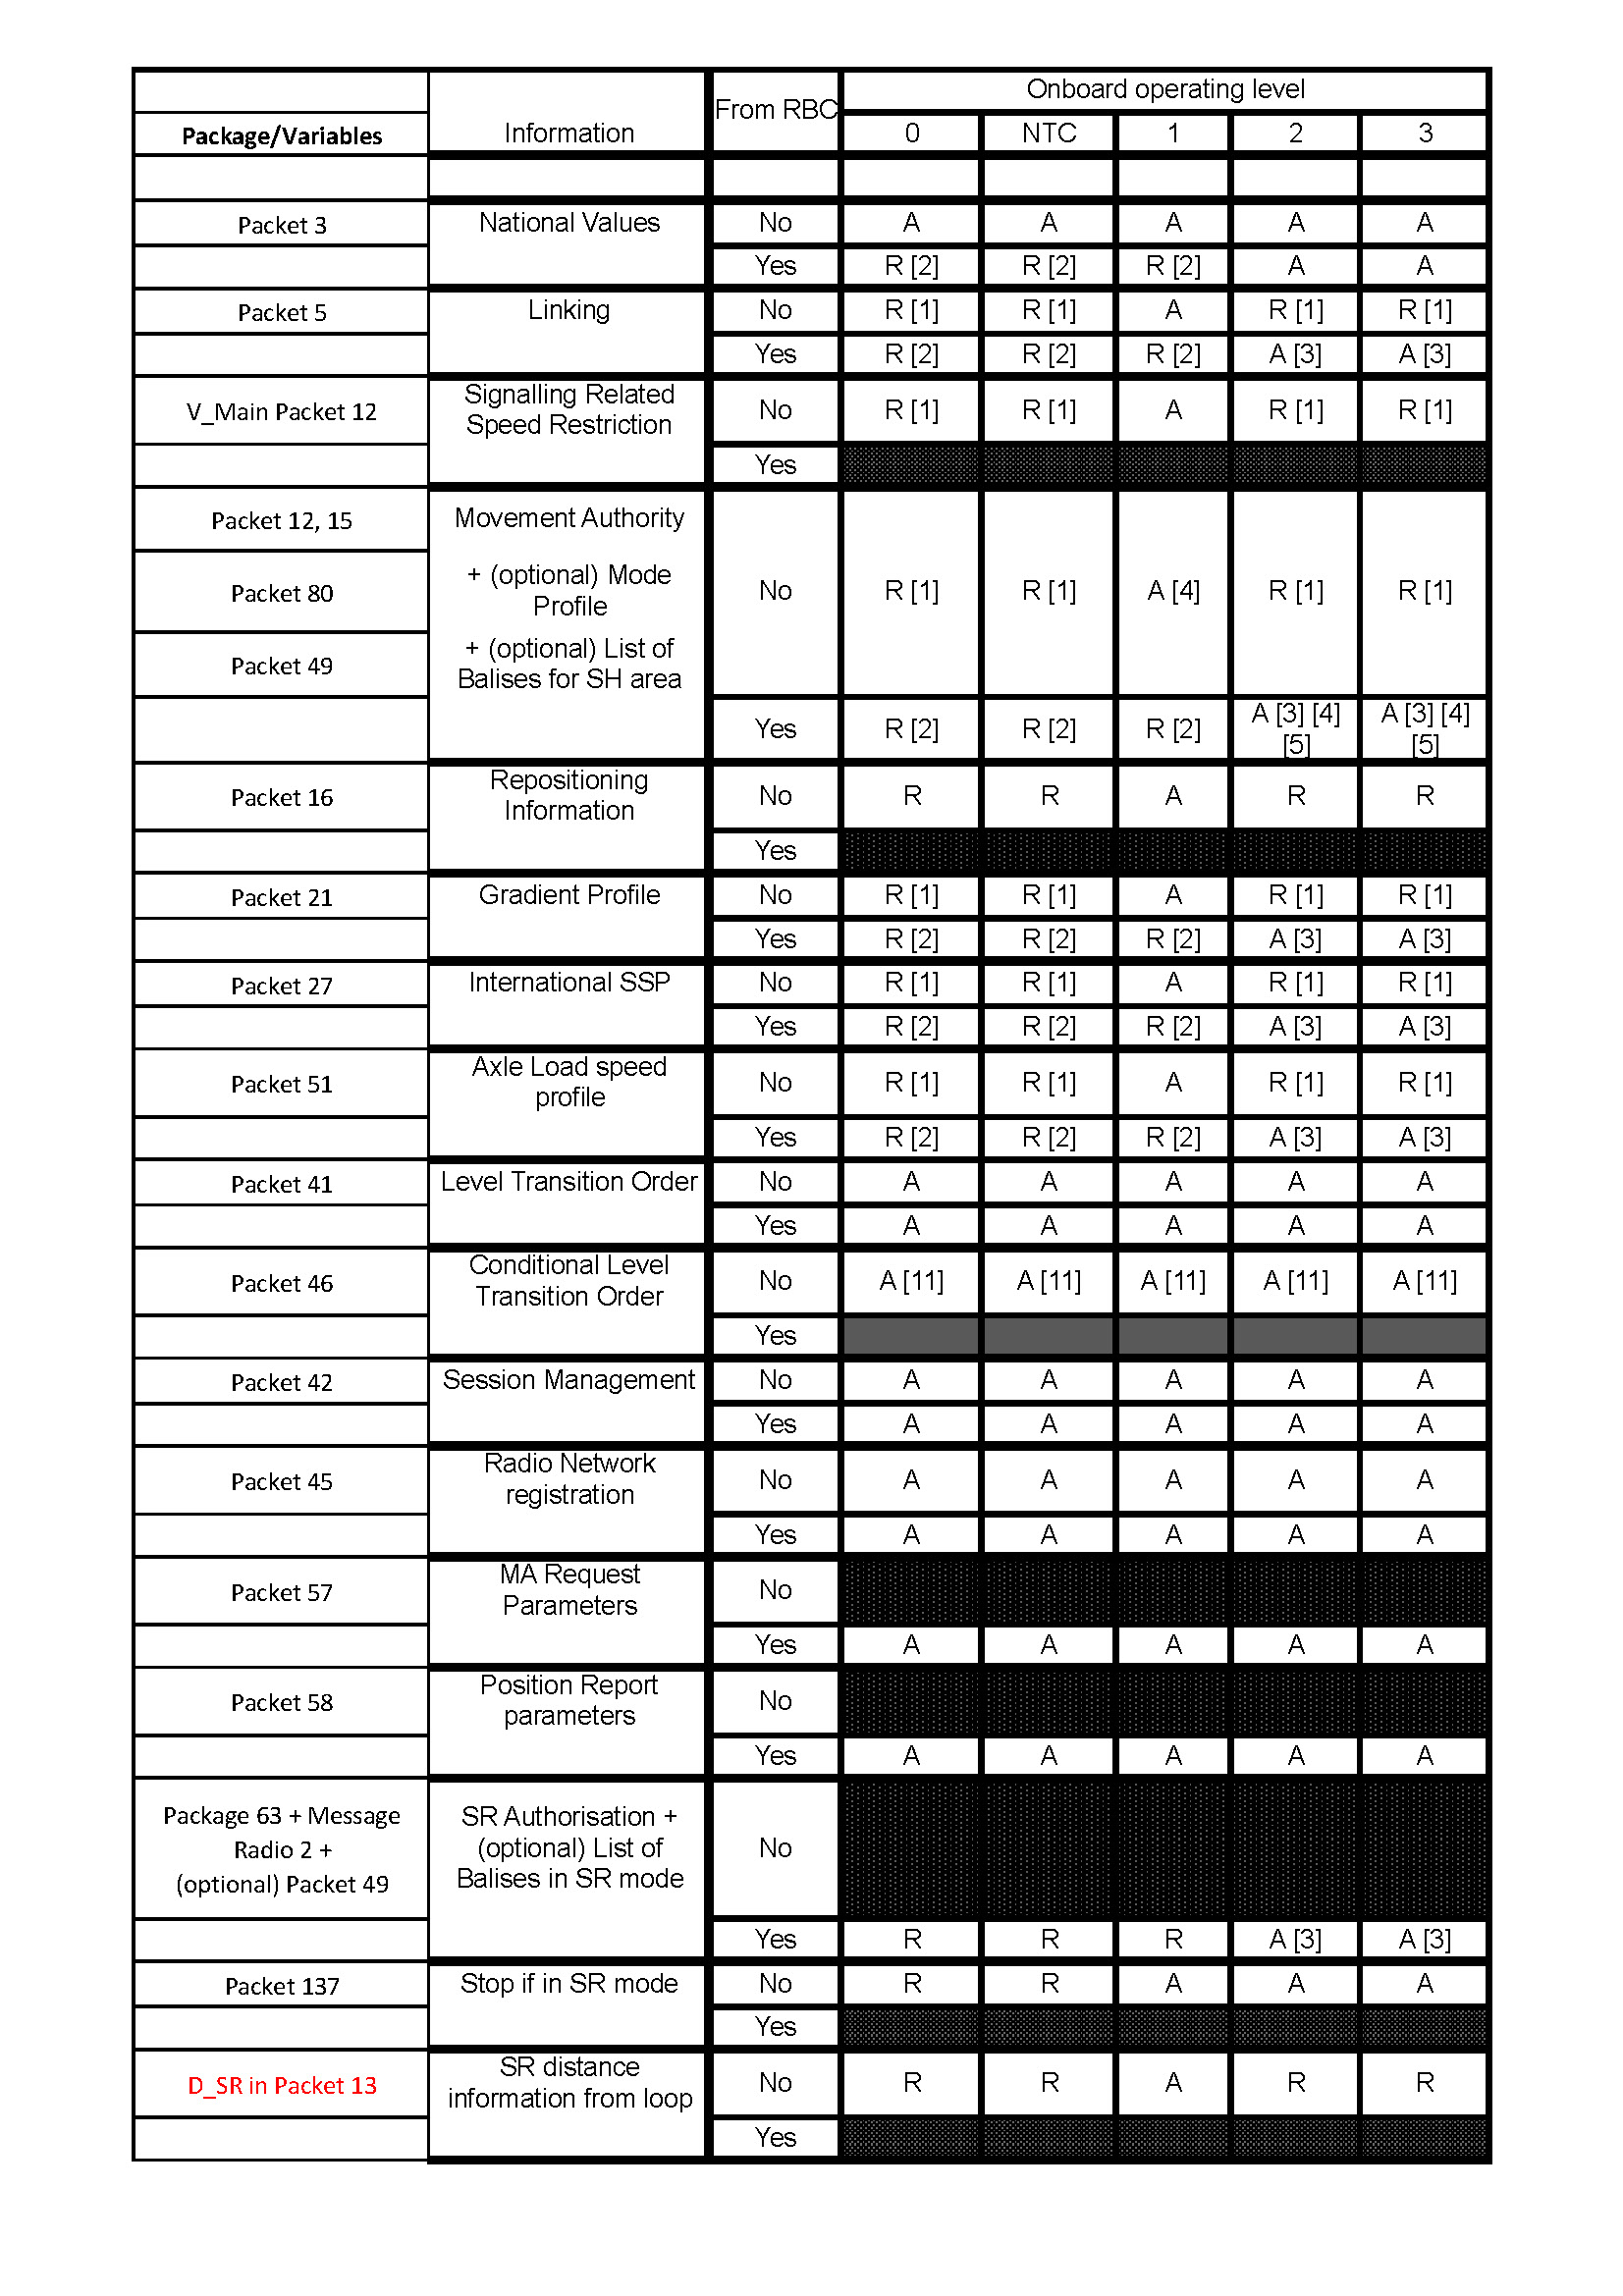
\includegraphics [scale=0.6]{images/LevelFilter1}
\end{figure}
\begin{figure}[hbtp]
\centering
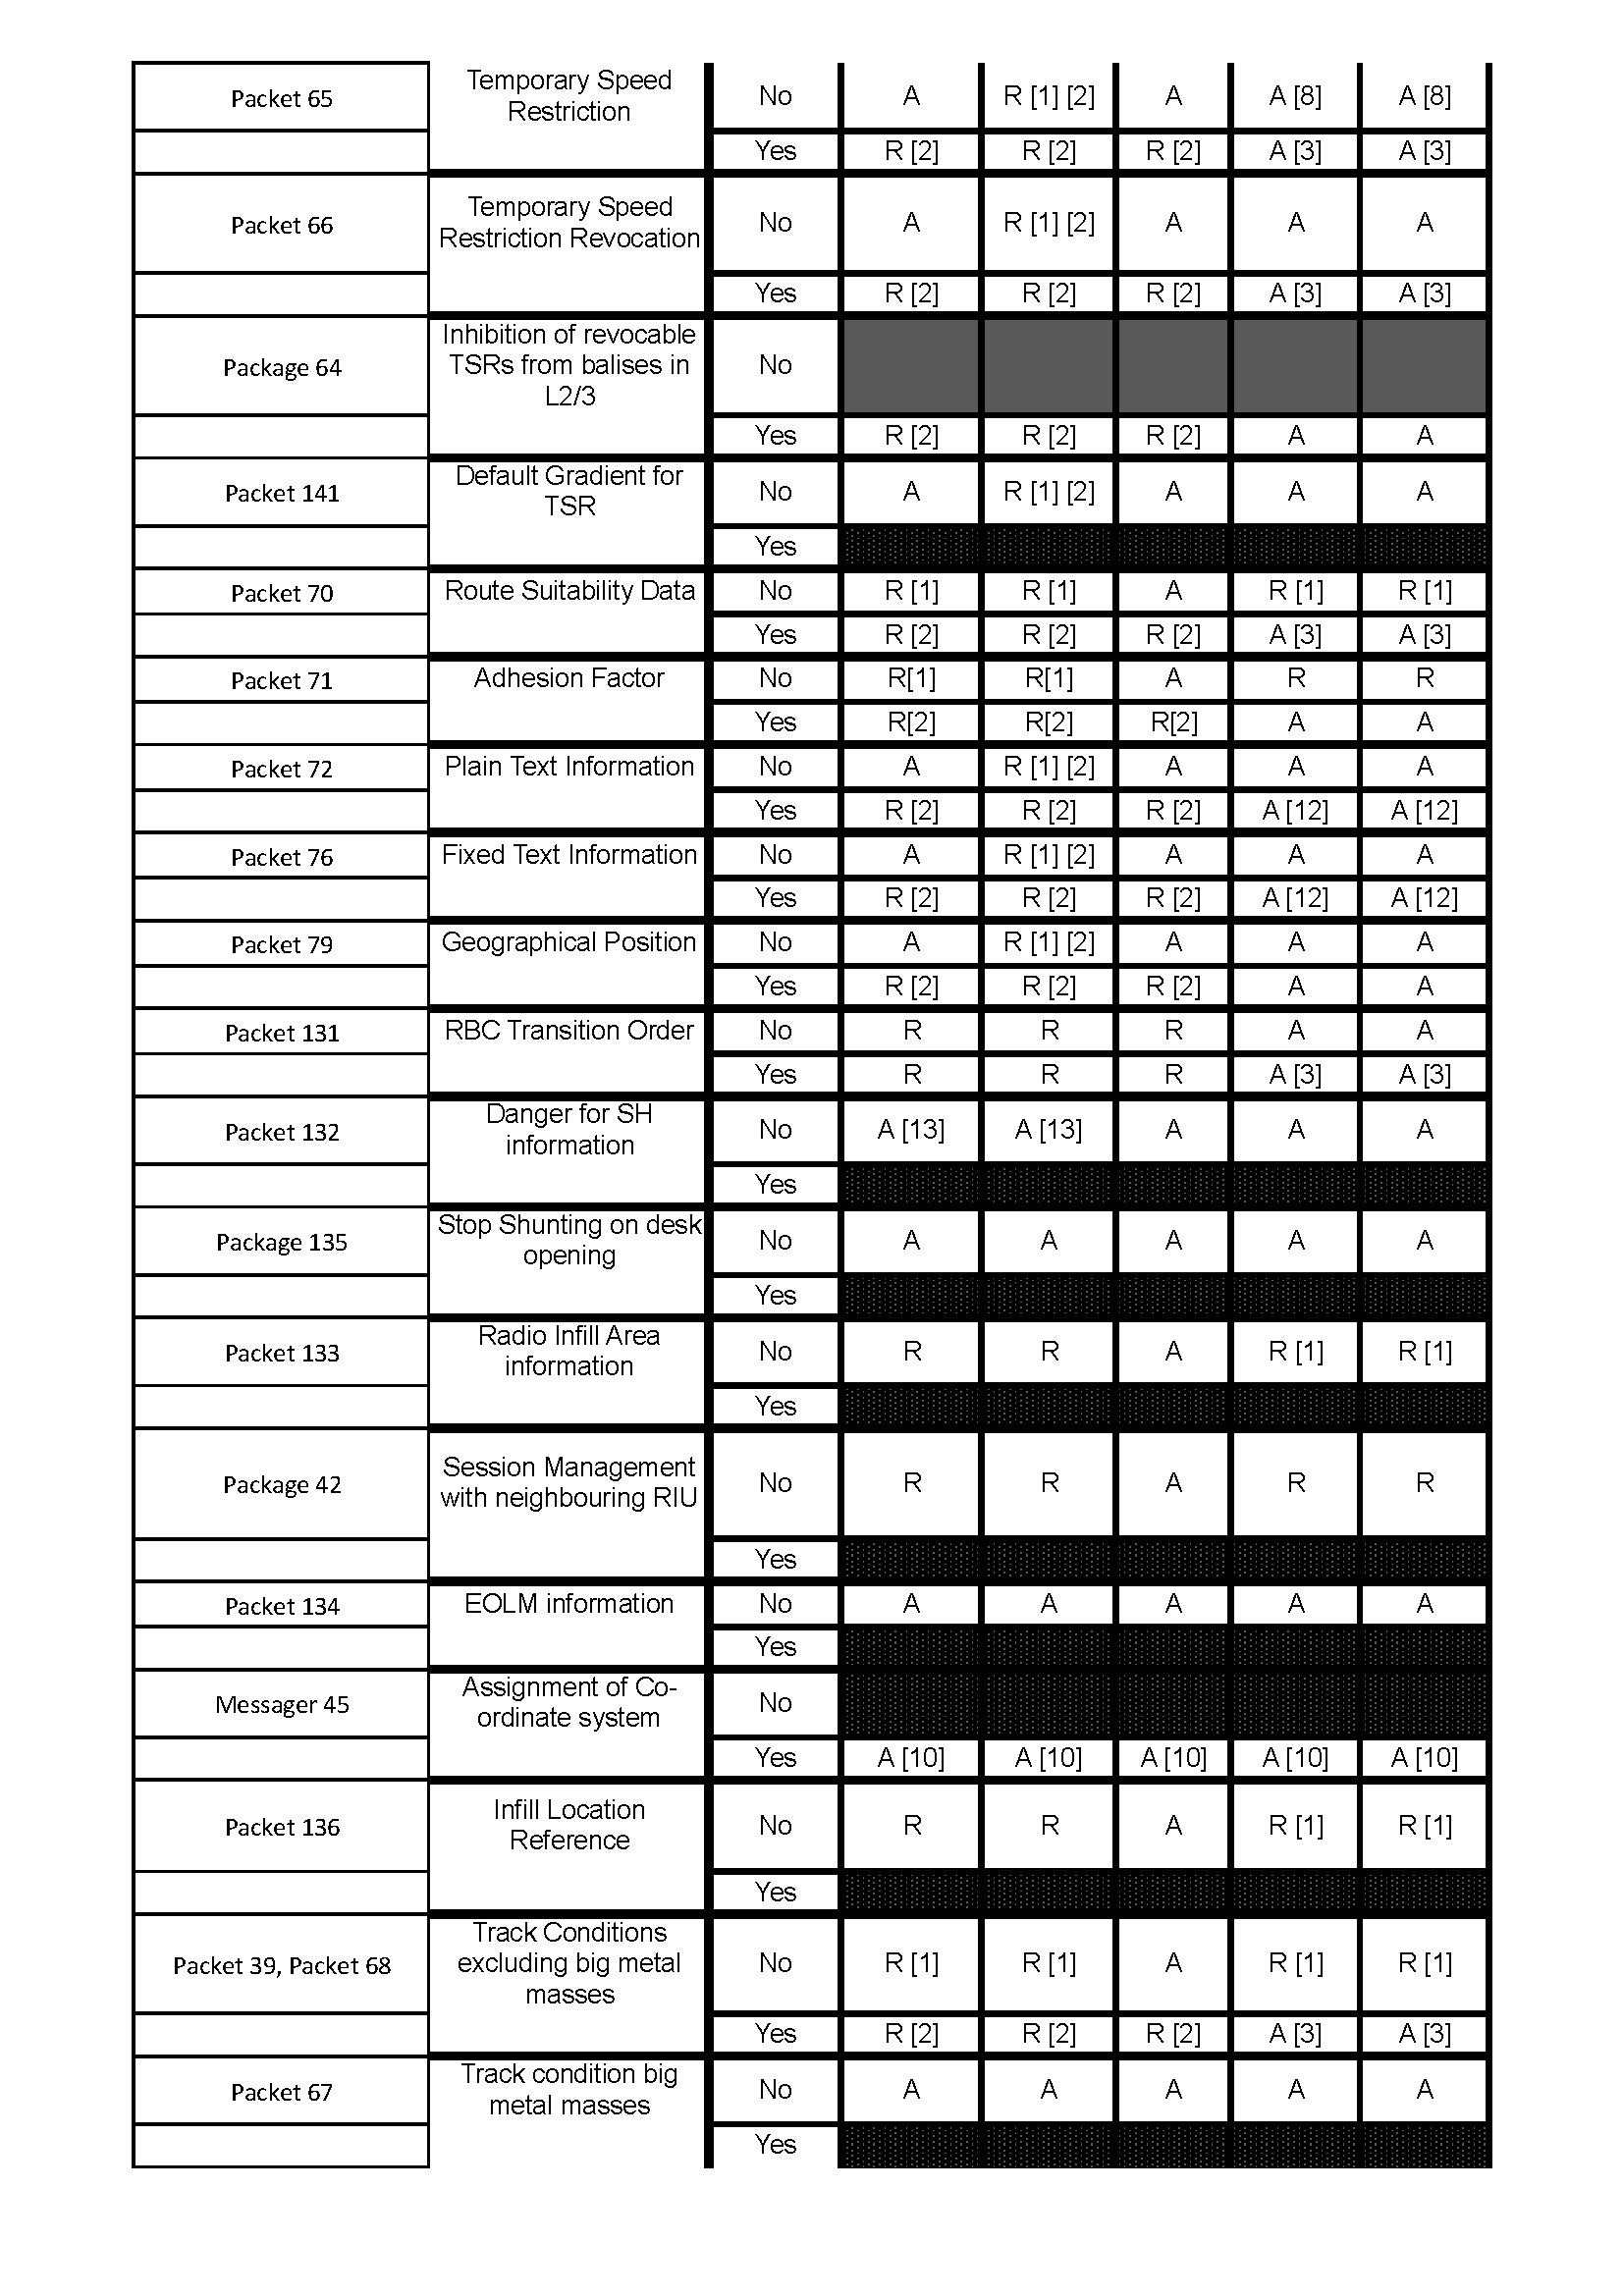
\includegraphics [scale=0.6]{images/LevelFilter2}
\end{figure}
\begin{figure}[hbtp]
\centering
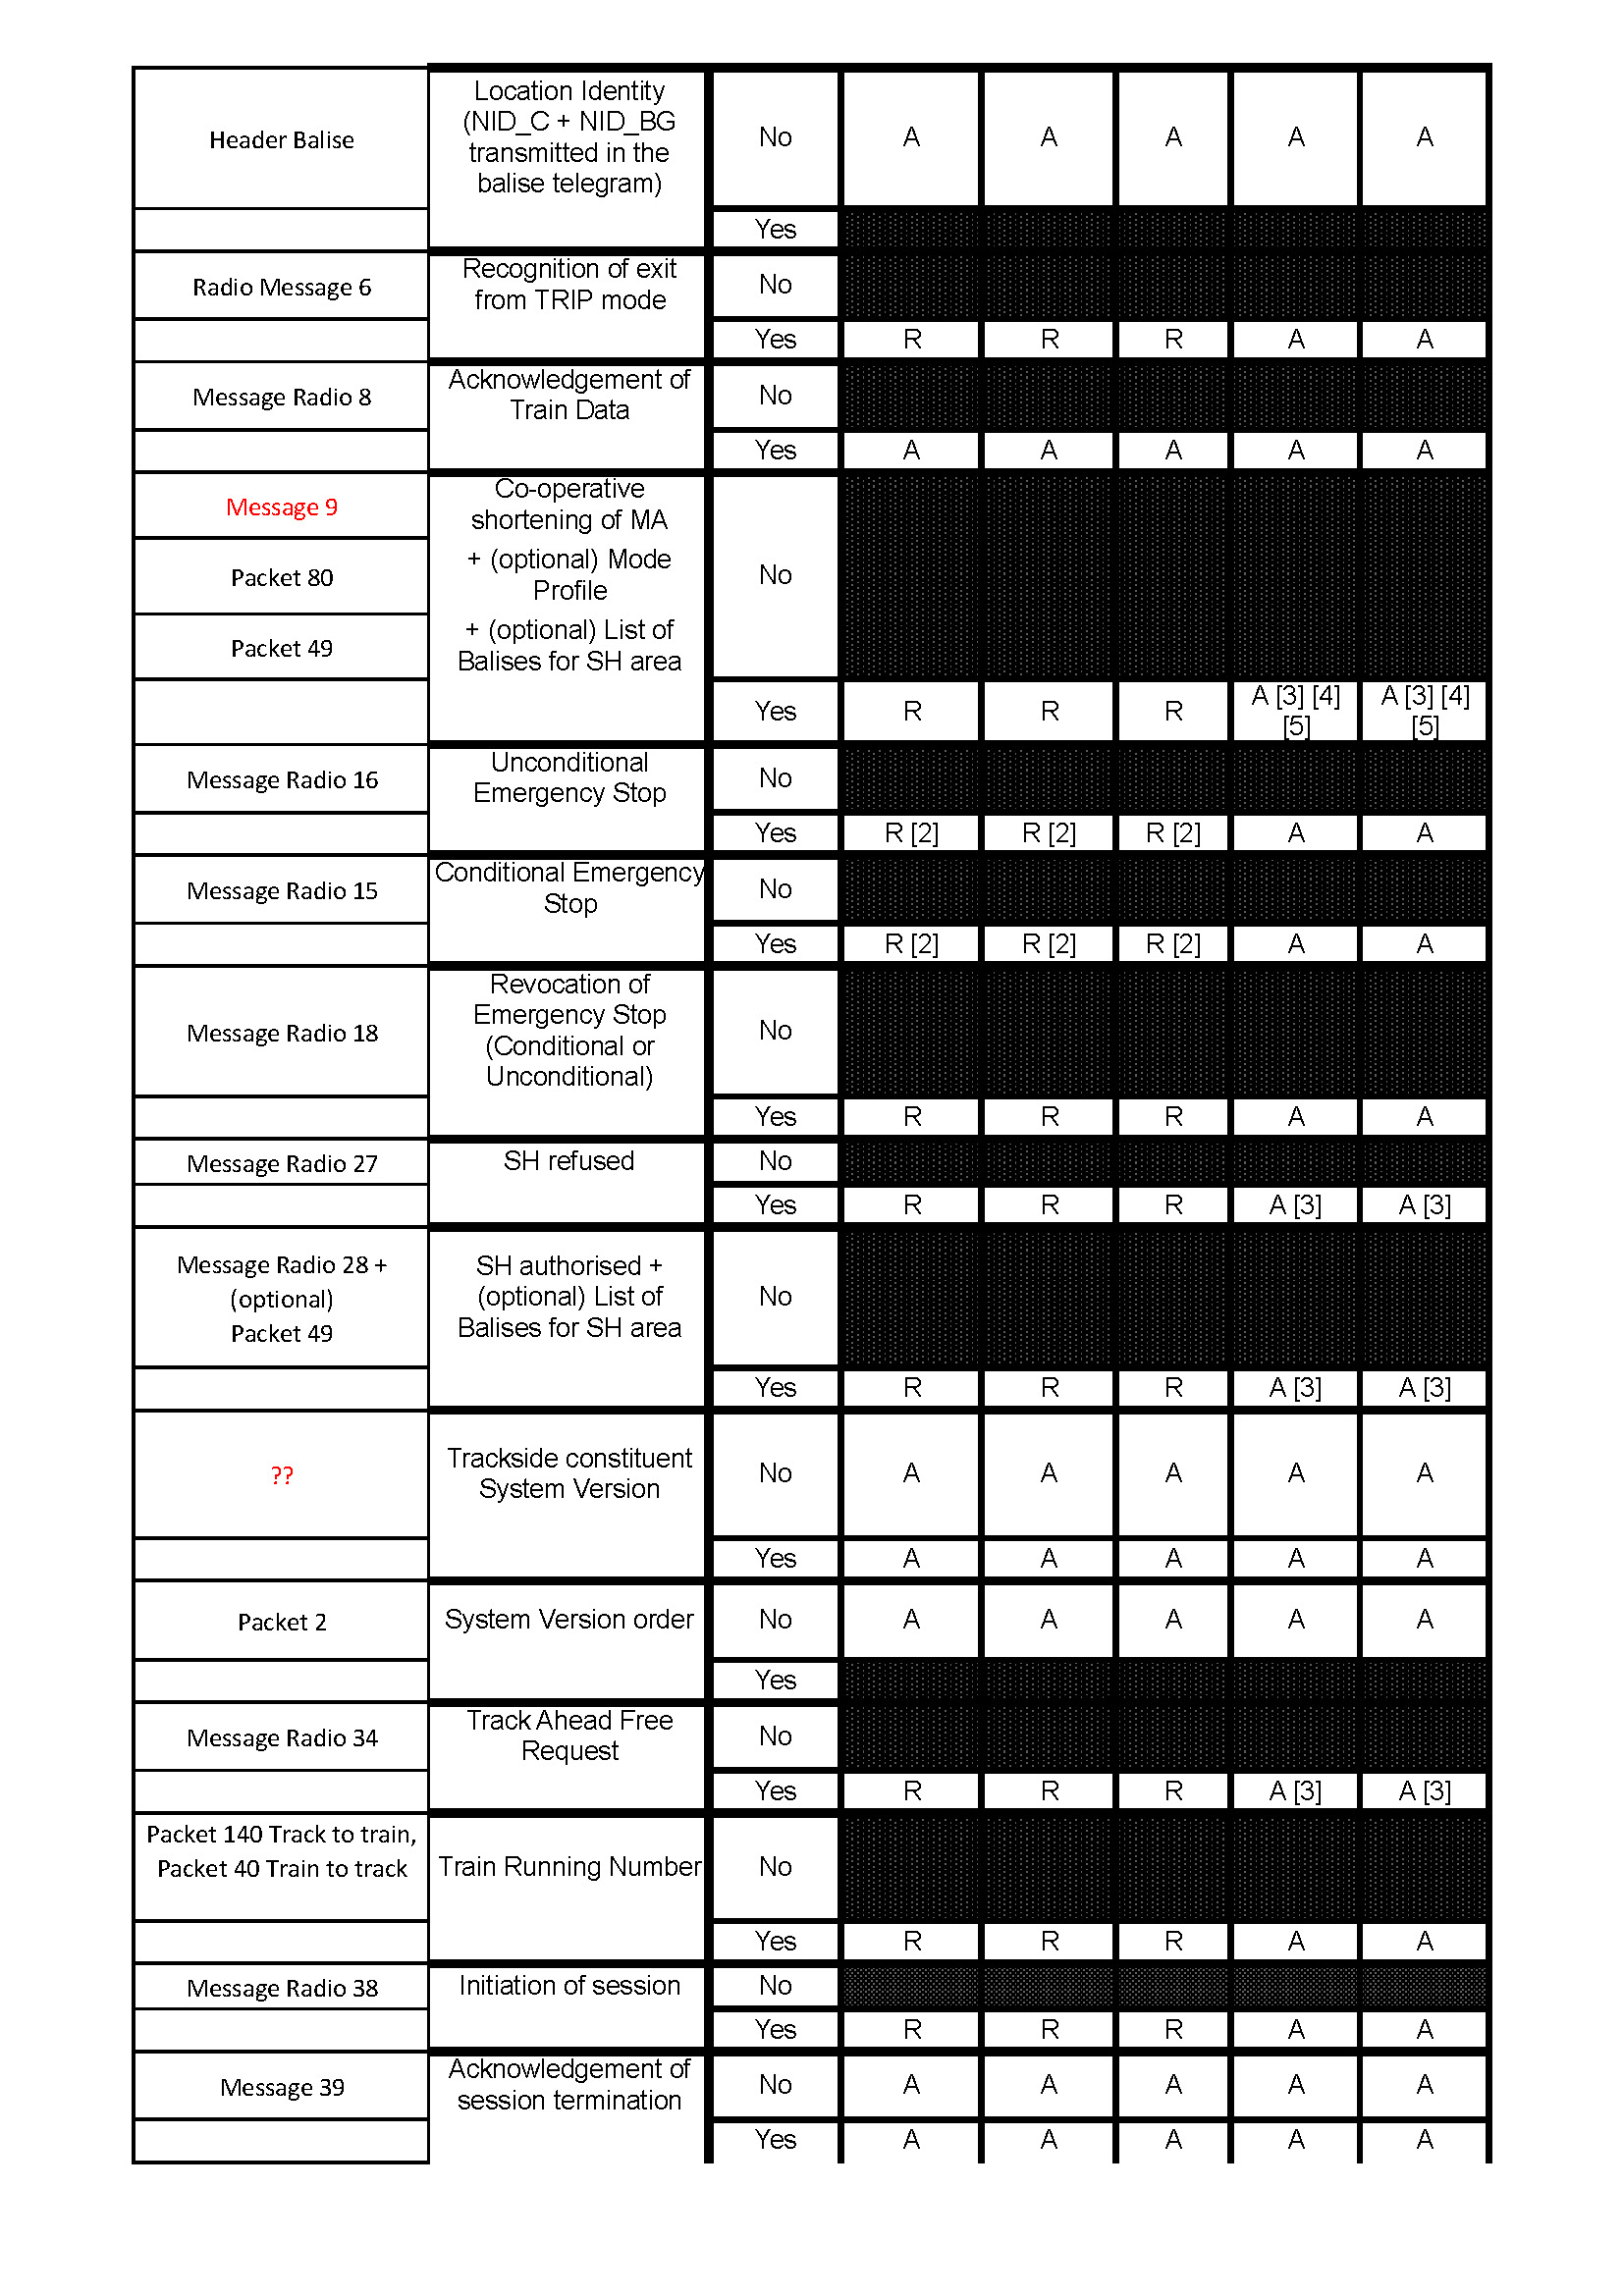
\includegraphics [scale=0.6]{images/LevelFilter3}
\end{figure}
\begin{figure}[hbtp]
\centering
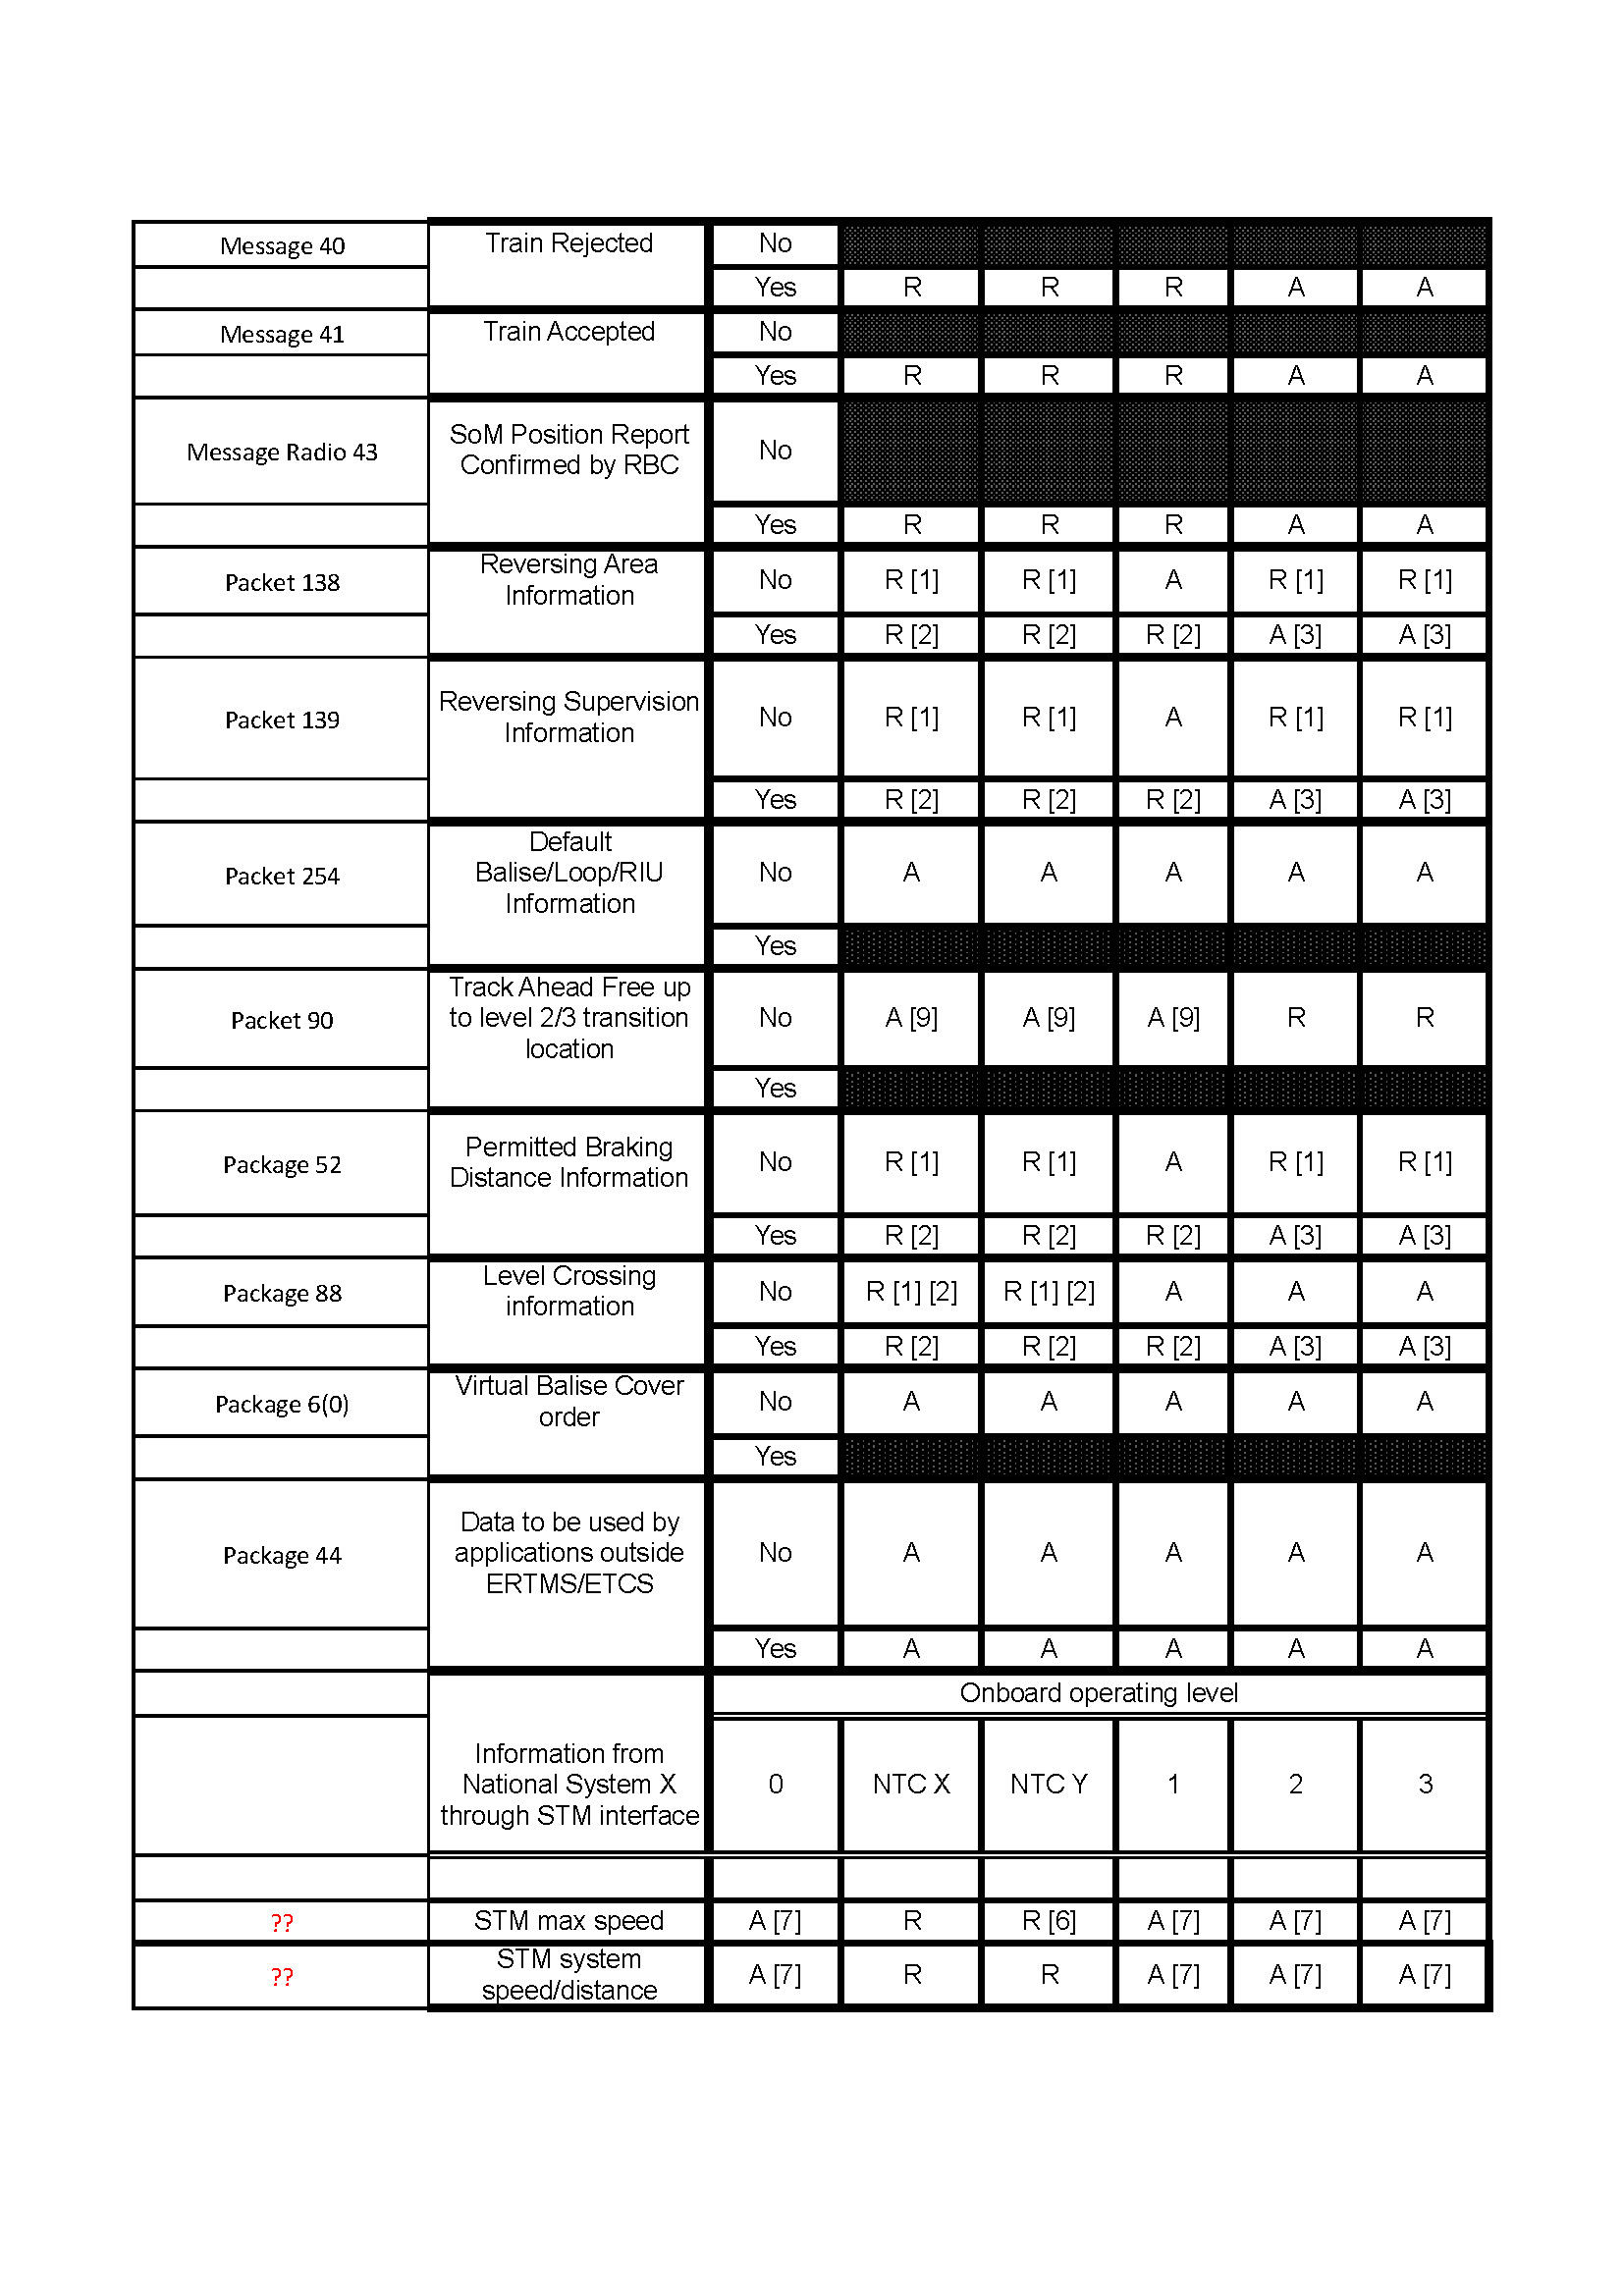
\includegraphics [scale=0.6]{images/LevelFilter4}
\caption{Lists of packages and their handling depending on train modes}
\label{fig:PackagesListLevel}
\end{figure}
\newpage

\begin{figure}[hbtp]
\centering
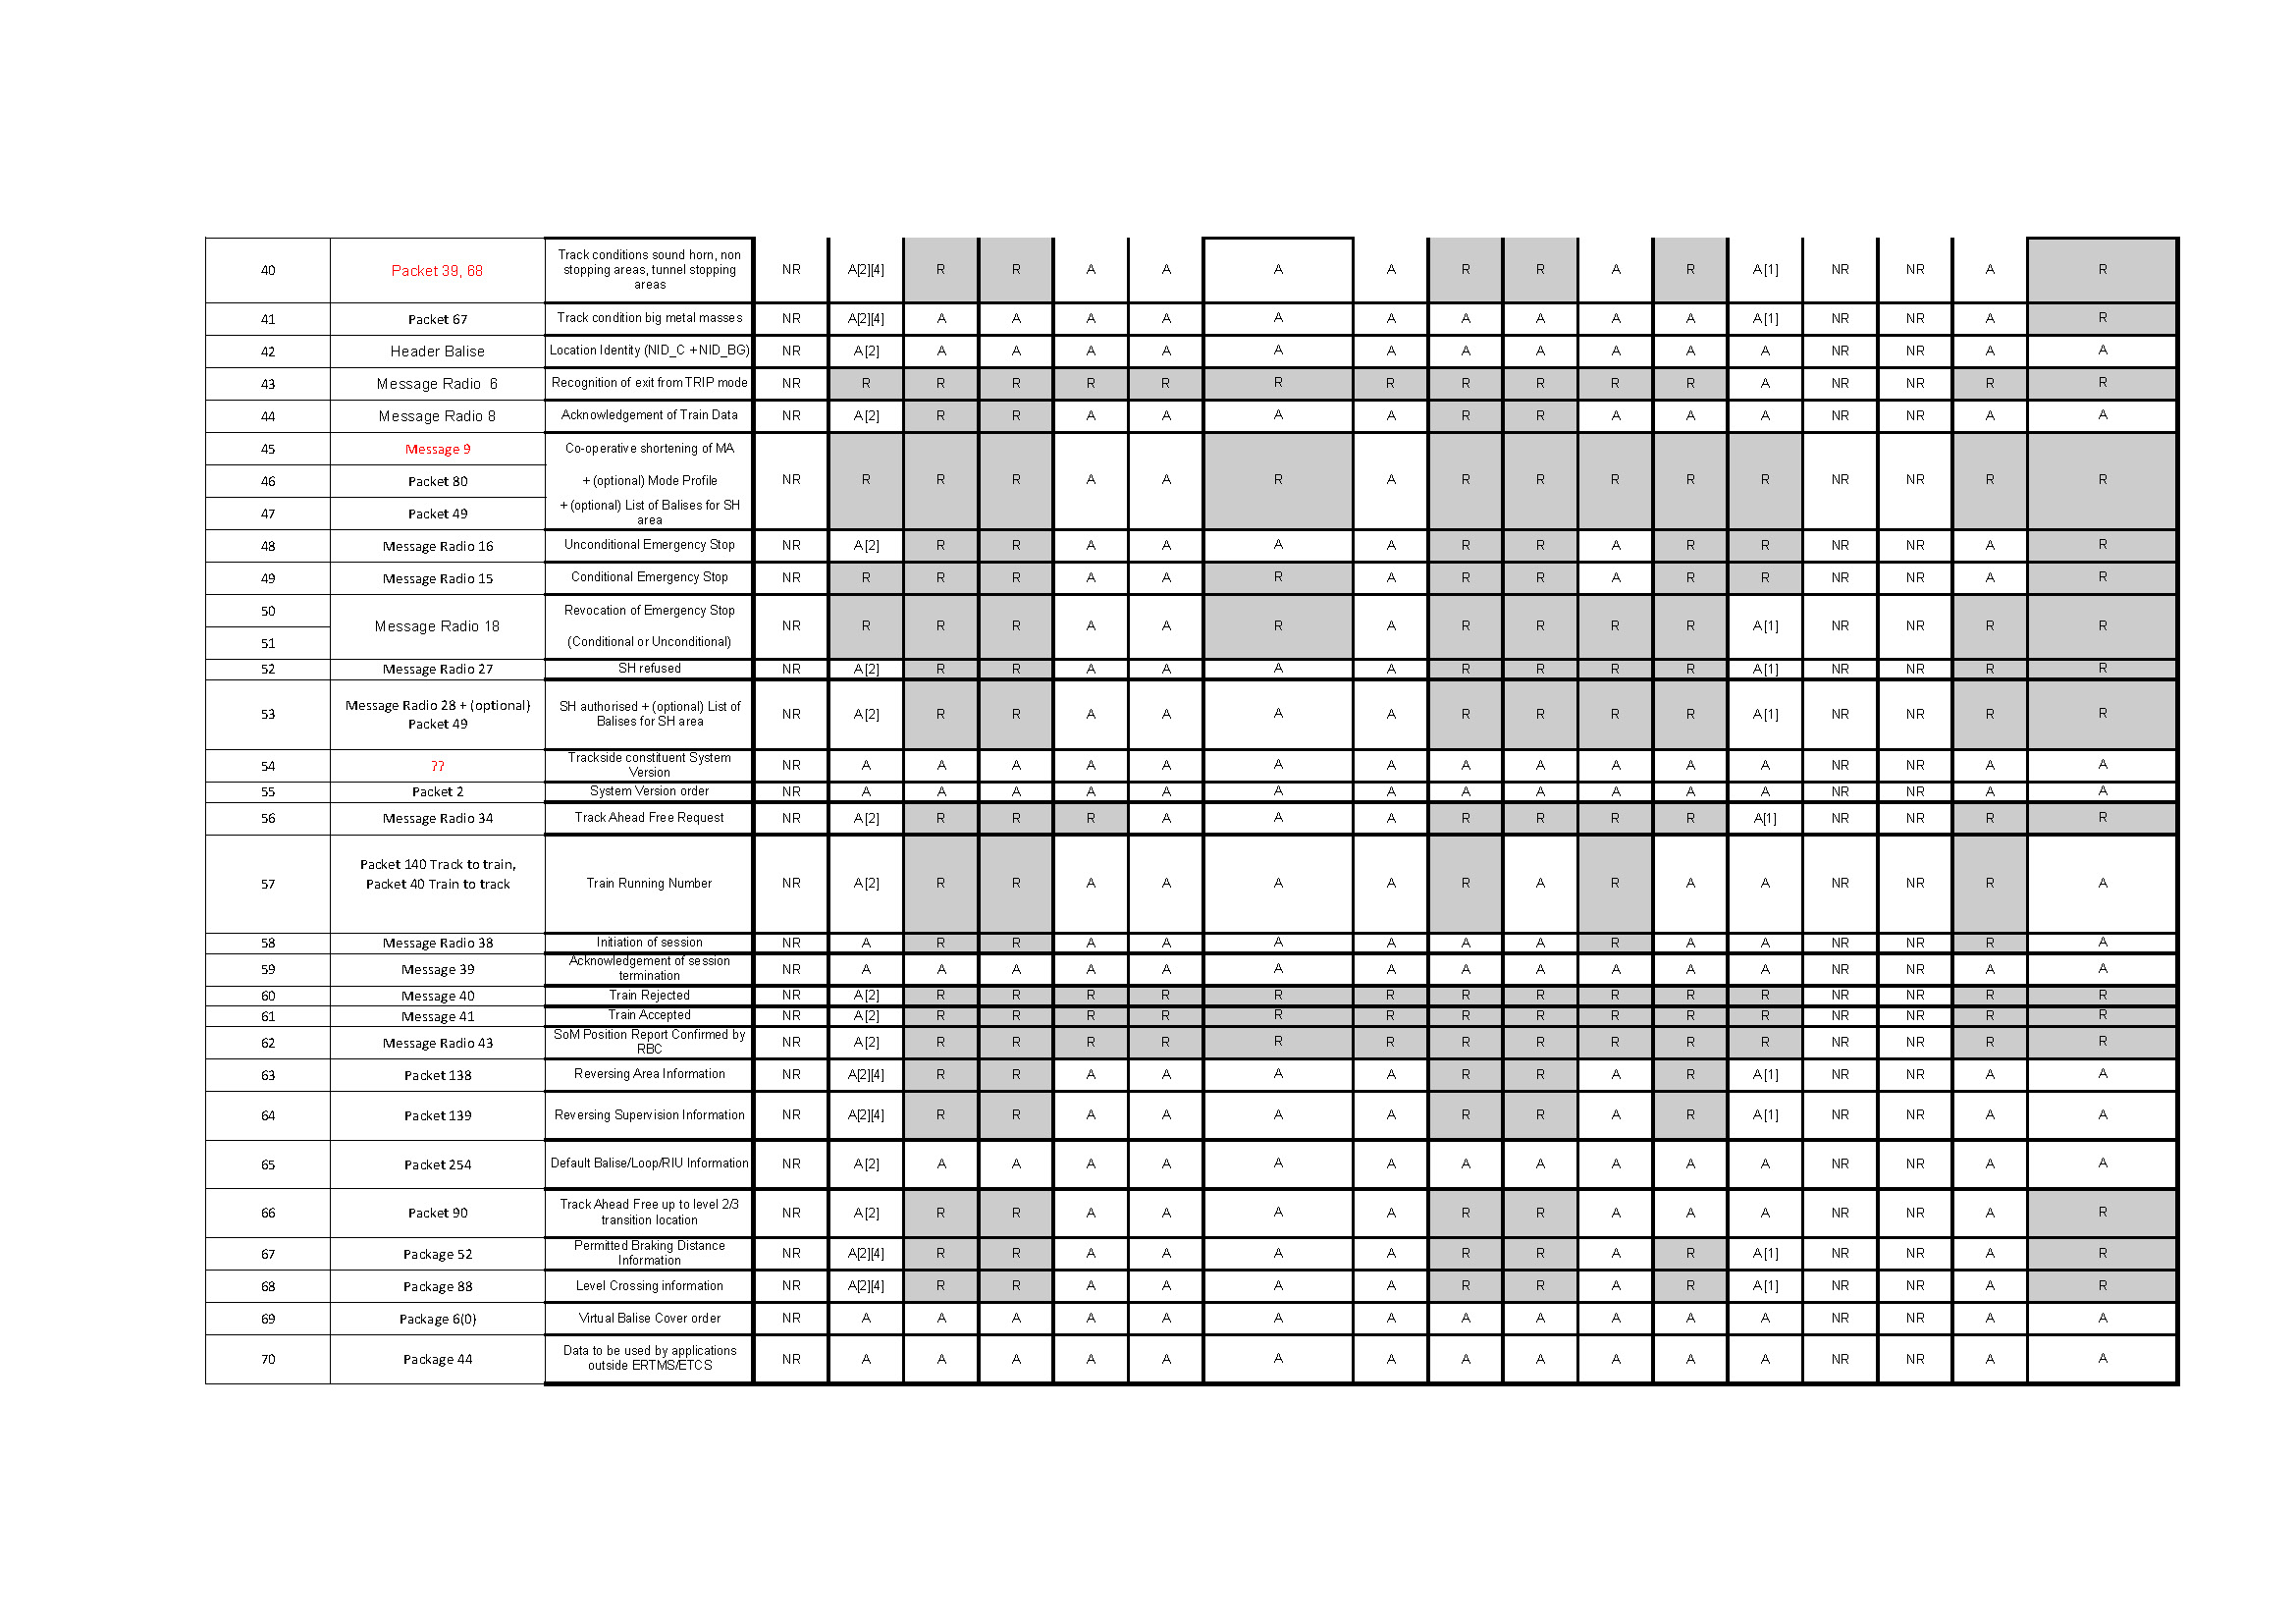
\includegraphics [angle=90, scale=0.8]{images/FilterMode1}
\end{figure}
\begin{figure}[hbtp]
\centering
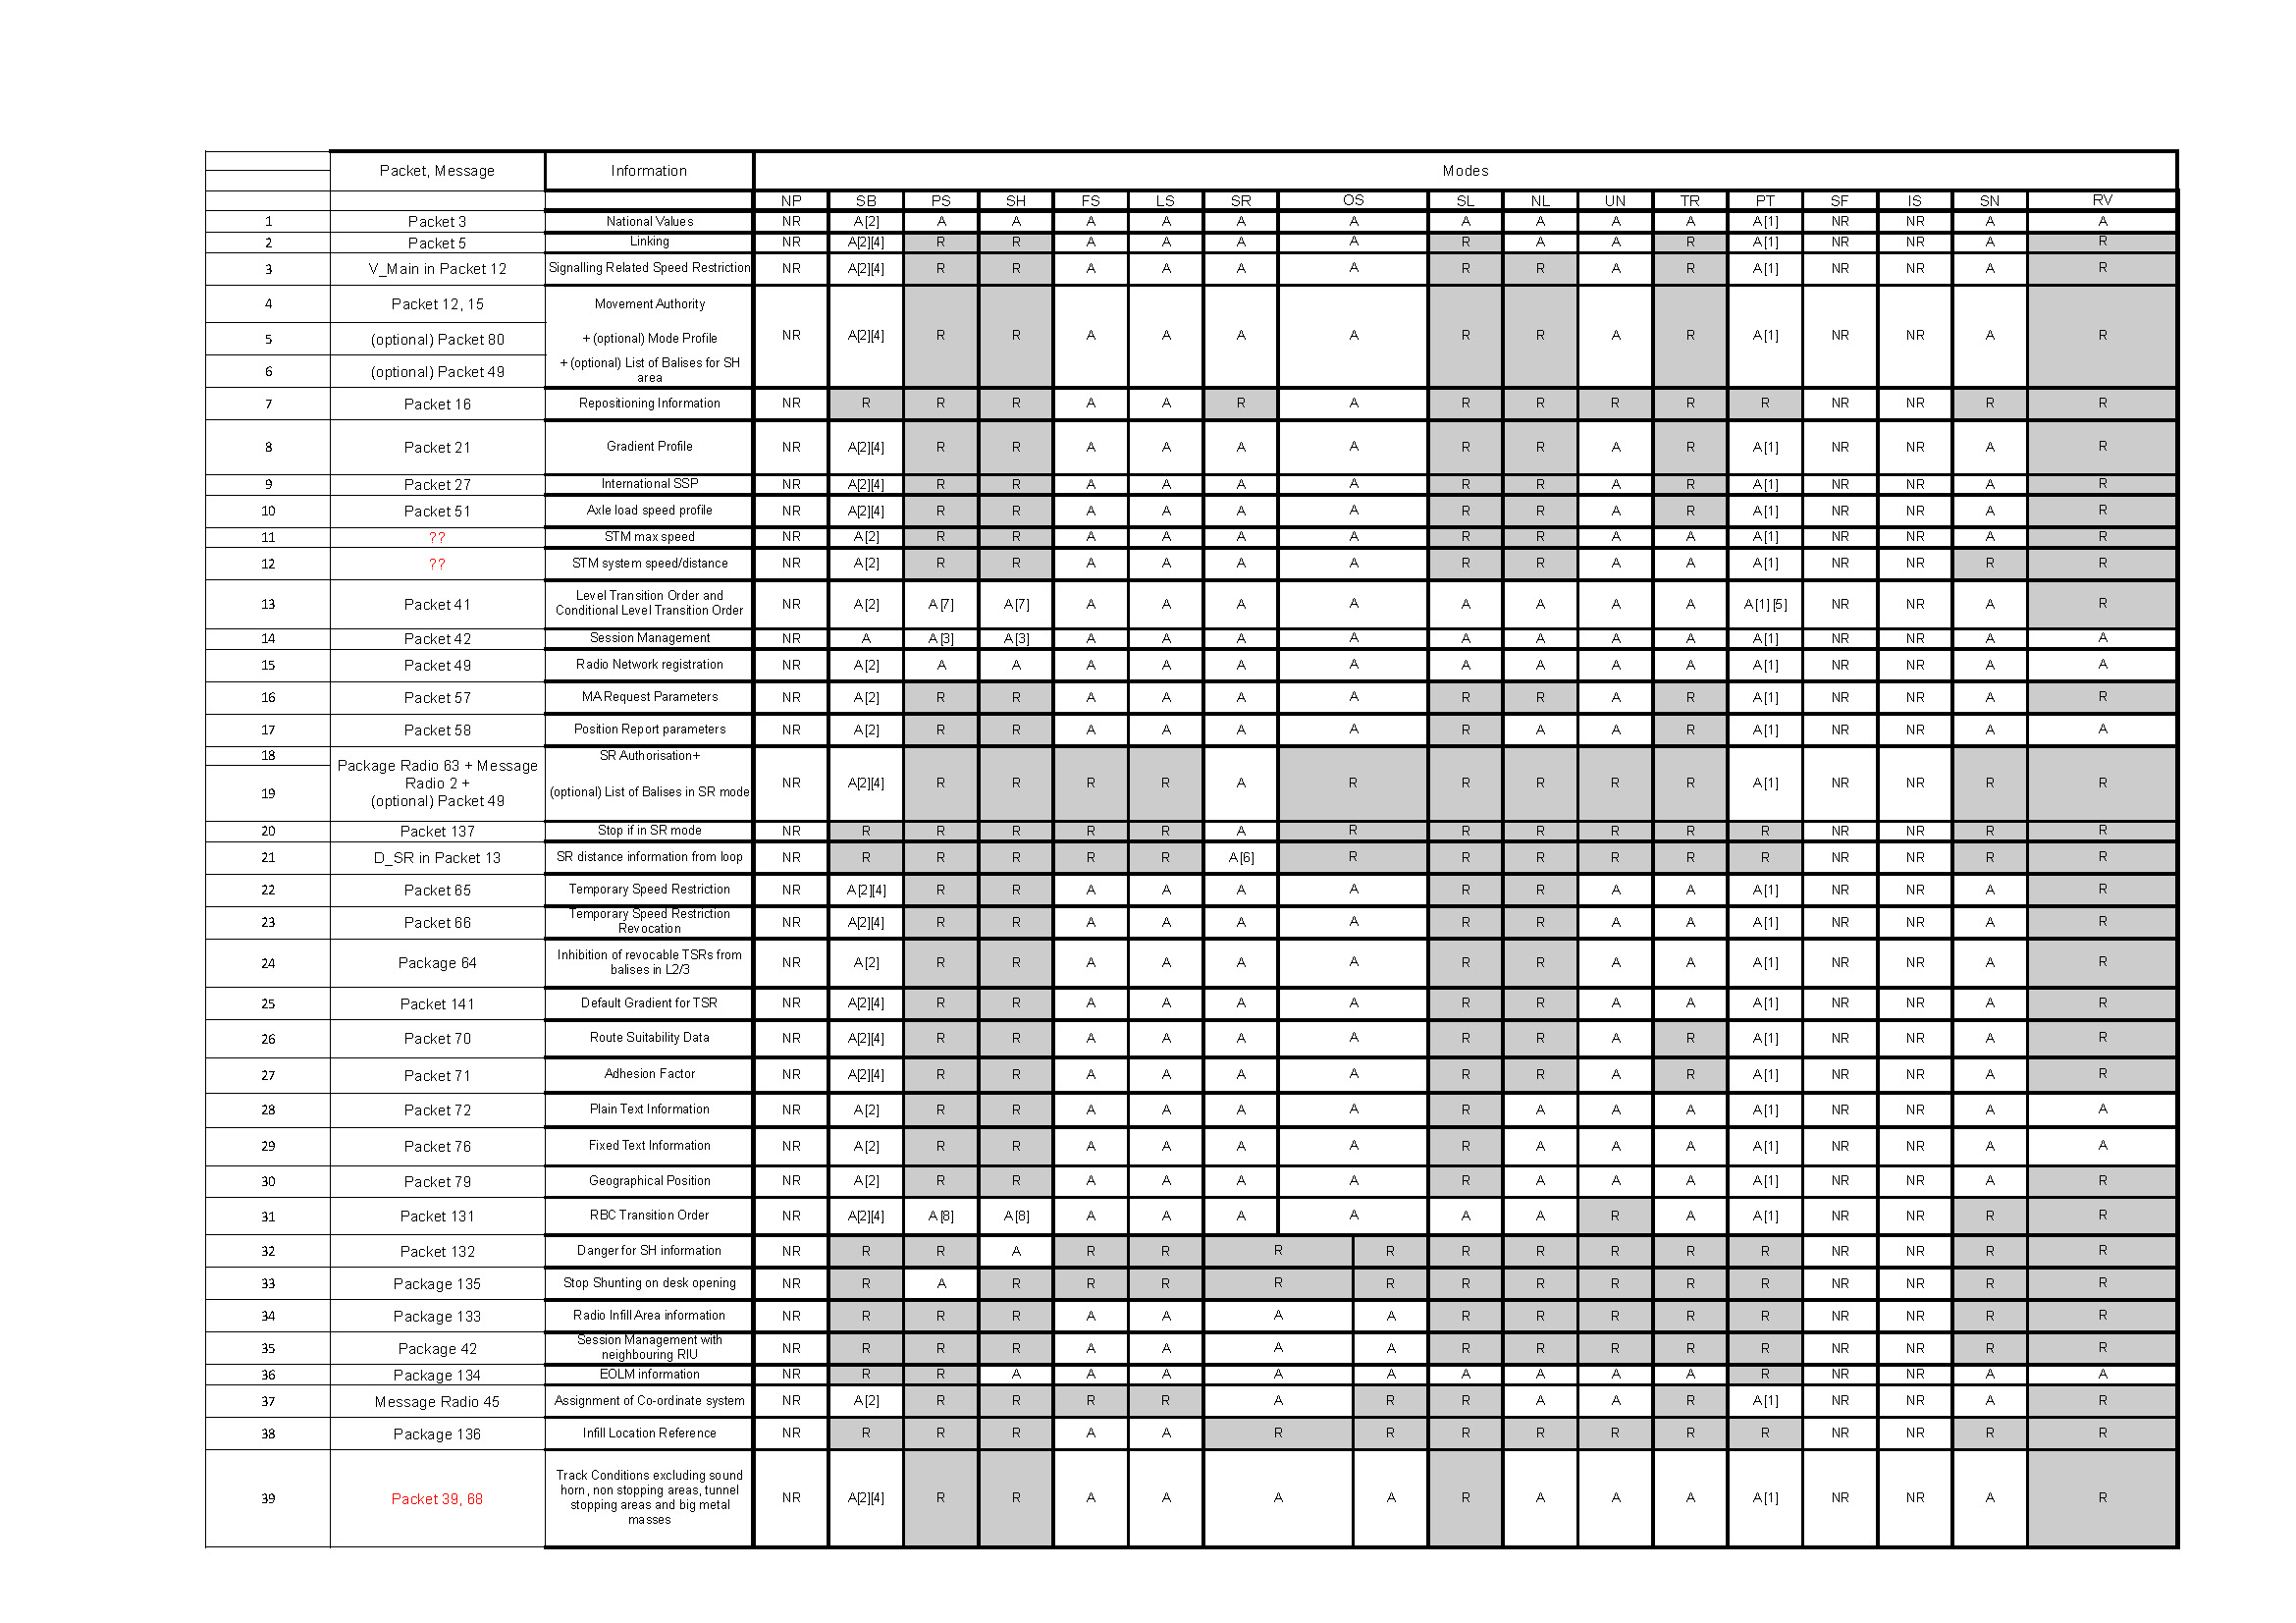
\includegraphics [angle=90, scale=0.8]{images/FilterMode2}
\end{figure}
\begin{figure}[hbtp]
\centering
\caption{Lists of packages and their handling depending on train modes}
\label{fig:PackagesListMode}
\end{figure}
\newpage

%%\subparagraph{Filtering (Mode/Level) - One packet per type}
%%\textbf{ISSUE: HOW MANY PKT 44, 65 AND 66 PER MESSAGE ARE MAXIMALLY SUPPORTED? (BH: who made this comment??)}\\

%% - Check on announced and immediate level transition orders in the messages to be filtered (needed for further criteria for filtering, to decide if the data shall be stored in the transition buffer).\\
%% - Filter data stored in the transition buffer according to the current level (what to do if similar information is available in the new message??). Data can be rejected, accepted or kept in the transition buffer.
%% (Filtering according to new level will be done directly afterwards in the next cycle)\\
%% - Filter new received messages according to the current level (new level will be done in the next cycle as according to \gls{SRS} data first has to be filtered according to old level and afterwards to new level). Data can be rejected, accepted or stored in the transition buffer.\\
%% - Filter (level) accepted data according to originating RBC (supervising or other). Information from \gls{BG}'s, loops or RIU is not filtered with this filter.\\
%% - Filter (level and RBC) accepted data according to the current mode (only reject or accept)\\


\paragraph{Reference to the Scade Model}
The SCADE model can be found on github under the following path:

\tiny\url{https://github.com/openETCS/modeling/tree/master/model/Scade/System/ObuFunctions/ManageLocationRelatedInformation/BaliseGroup/InformationFilter}
\normalsize%Mainfunction receive track data. Name should be be defined and substituded by the designer of the function. 

%set the master document for easy compilation
%!TEX root = ../D3_5_2.tex

%-----------------------------------------------------------------------
\section{Train Supervision}
%-----------------------------------------------------------------------
%\tbc
%Group 1 (Christian Stahl)

\begin{figure}
\centering
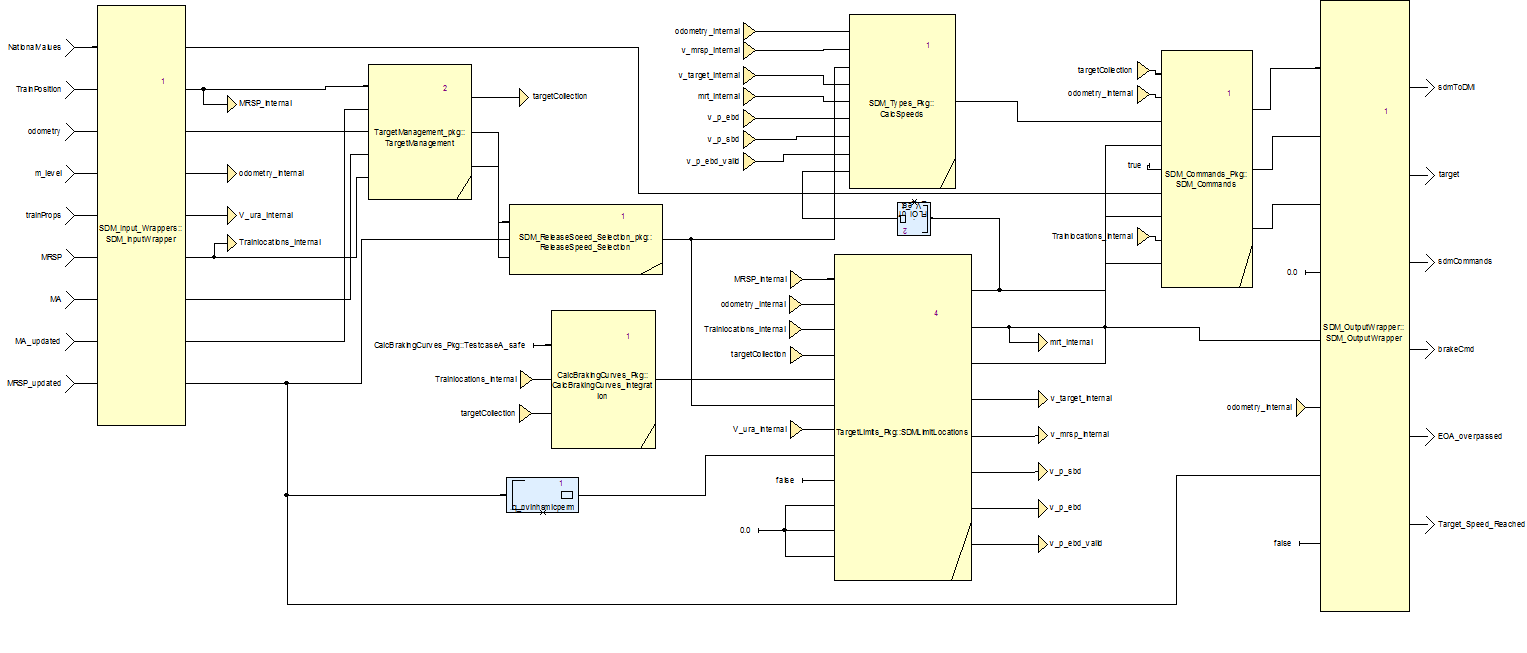
\includegraphics[width=0.95\textheight, angle=90]{../images/speedsupervision.png}
\caption{Structure of component ProvidePositionReport}\label{fig:ssv}
\end{figure}

The task of block ``Train Supervision'' is to monitor the speed of the train and the train location and as such to ensure that the speed remains within the given speed and distance limits. This block is mainly based on \cite[Chapt.~3.13]{subset-026}.

The block ``Train Supervision'' takes as input (1) movement related information such as train speed, train position and acceleration, (2) train related information such as brake information and train length, and (3) track related information such as speed and distance limits and national values.

Based on this information a speed profile is calculated. Speed restrictions create target speeds (targets) that have to be followed. For each such target braking curves are generated to supervise at which location of the track the train must perform the brake. In case of no target restrictions the train may accelerate to the supervised maximum speed of the speed profile. These calculations lead to commands being sent to the driver and the brake system.

The functionality is modeled using eight operators, as shown in Figure~\ref{fig:ssv}, which are explained below.

The current status of the analysis of ``Train Supervision'' and a functional breakdown can be found in a separate document, \verb+SpeedSupervision_analysis.pdf+.



\subsection{Input}
For providing the output, the module needs different input data flows. Table \ref{tbl:speedsupervisionInput} gives an overview.

\begin{table}[H]
  \begin{tabular}{| c | l | l | l | l |}
    \hline
    \textbf{Index} & \textbf{Input name} & \textbf{Input type} & \textbf{Source}\\ \hline
    0 & \texttt{NationalValues} & \texttt{P3\_NationalValues\_T} & ???\\
    1 & \texttt{TrainPosition} & \texttt{trainPosition\_T} & Manage Track Data\\
    2 & \texttt{odometry} & \texttt{odometry\_T} & Odometry\\
    3 & \texttt{m\_level} & \texttt{M\_LEVEL} & Mode and Level\\
    4 & \texttt{trainProps} & \texttt{trainProperties\_T} & Database\\
    5 & \texttt{MRSP} & \texttt{MRSP\_Profile\_t} & ?? \\
    6 & \texttt{MA} & \texttt{MAs\_t} & ??\\
    7 & \texttt{MA\_updated} & \texttt{bool} & internal\\
    8 & \texttt{MRSP\_updated} & \texttt{bool} & internal\\
    \hline
  \end{tabular} 
  \caption{Overview of inputs}
  \label{tbl:speedsupervisionInput}
\end{table}

\subsubsection{Input 0: \texttt{NationalValues}}
This input is packet 3 of \cite[Chapt.~8]{subset-026}, describing the national values. 
\subsubsection{Input 1: \texttt{TrainPosition}}
This input is the current train position.
\subsubsection{Input 2: \texttt{odometry}}
This input is the odometry data.
\subsubsection{Input 3: \texttt{m\_level}}
This input is the current level of the train.
\subsubsection{Input 4: \texttt{trainProps}}
This input is a set of train related properties.
\subsubsection{Input 5: \texttt{MRSP}}
This input is the most restrictive speed profile.
\subsubsection{Input 6: \texttt{MA}}
This input is a movement authority.
\subsubsection{Input 7: \texttt{MA\_updated}}
This flag is true if the movement authority has been updated in this clock cycle and false otherwise.
\subsubsection{Input 8: \texttt{MRSP\_updated}}
This flag is true if the most restrictive speed profile has been updated in this clock cycle and false otherwise.



\subsection{Output}
Based on the input the block produces the following output. Table~\ref{tbl:speedsupervisionOutput} gives an overview.

\begin{table}[H]
  \begin{tabular}{| c | l | l | l |}
    \hline
    \textbf{Index} & \textbf{Output name} & \textbf{Output type}\\ \hline
    0 & \texttt{sdmToDMI} & \texttt{speedSupervisionForDMI\_T}\\
    1 & \texttt{target} & \texttt{Target\_T}\\
    2 & \texttt{sdmCommands} & \texttt{SDM\_Commands\_T}\\
    3 & \texttt{brakeCmd} & \texttt{Brake\_command\_T}\\
    4 & \texttt{EOA\_overpassed} & \texttt{bool}\\
    5 & \texttt{Target\_Speed\_Reached} & \texttt{bool}\\
    \hline
  \end{tabular} 
  \caption{Overview of outputs}
  \label{tbl:speedsupervisionOutput}
\end{table}

\subsubsection{Output 0: \texttt{sdmToDMI}}
This output contains information about different speeds and positions, on the one hand and the current supervision status, on the other hand. This information shall be displayed to the driver.
\subsubsection{Output 1: \texttt{target}}
This output is the most restrictive displayed target (MRDT).
\subsubsection{Output 2: \texttt{sdmCommands}}
This output gives some intermediate results of operator SDM\_Commands. It is currently used for test purposes only.
\subsubsection{Output 3: \texttt{brakeCmd}}
This output is the brake command, indicating whether performing the service brake or the emergency brake have been commanded.
\subsubsection{Output 4: \texttt{EOA\_overpassed}}
This output is true if the end of authority has been overpassed and false otherwise.
\subsubsection{Output 5: \texttt{Target\_Speed\_Reached}}
This output is true if the current speed is greater than or equal the target speed and false otherwise.



\subsection{SDM\_InputWrapper in Train Supervision}

\subsubsection{Reference to the SRS or other Requirements (or other requirements)}
\begin{itemize}
	\item \cite[Chapt.~3.13]{subset-026}: Speed and distance monitoring 
\end{itemize}

\subsubsection{Short description of the functionality}
The motivation for this operator is to convert all inputs of block ``Speed Supervision'' that contain information about length, speed, distance, and acceleration defined as integer into \texttt{real} to allow automatically the highest precision in the calculations by the meaning of floating point operations. In addition, to ease the modeling, inside block ``Speed Supervision'' only units meters ($[m]$), seconds($[s]$), meters per second($[\frac{m}{s}]$), and meters per square second($[\frac{m}{s^{2}}]$) are used.

\subsubsection{Interface}

\subsubsection{Functional Design Description}
This operator forwards input messages, takes data from complex data types or transforms inputs messages into an internal type thereby converting int to real.
  
\subsubsection{Reference to the Scade Model}

\subsection{TargetManagement in Train Supervision}

\subsubsection{Reference to the SRS or other Requirements (or other requirements)}
\begin{itemize}
	\item \cite[Chapt.~3.13.8.2]{subset-026}: Determination of the supervised targets 
\end{itemize}

\subsubsection{Short description of the functionality}
This operator calculates/updates the list of targets to be supervised by the block ``Train Supervision''. Taking the current movement authority, the most restrictive speed profile and the current maximum safe front end position as an input, the operator outputs a single End of Authority target, a list of all MRSP-Targets and a list of all LoA-Targets.
  
\subsubsection{Interface}

\subsubsection{Functional Design Description}
\paragraph{Derivation of Targets from Movement Authority Sections}
The sections of the \emph{Movement Authority} could cause two types of targets:
\begin{description}
\item[End Of Authority(EoA)] only one could exist and this is only in the \emph{end section} of the \emph{MA}
\item[Limit of Authority (LoA)] is possibly in every section of the \emph{MA} except the end section
\end{description}
In every cycle in which the MA is updated, the operator iterates through the entire MA and puts all speed limitations by \emph{LoA}s into a list of targets. The end section is used to derived the \emph{EoA} target. All LoA targets are sorted by location.

\paragraph{Derivation of Targets from MRSP}
According to \cite[Chapt.~3.13.8.2]{subset-026}, every speed decrease of the MRSP is used to derive a target. Therefore in every cycle in which the MRSP is updated, the operator iterates through the entire MRSP searching for all MRSP targets. For this purpose, every element of the MRSP is compared with its successor.

\paragraph{Update of Targets}
In every cycle the operator monitors whether all targets are already passed. To this end, it iterates over the list of targets comparing the current max safe front end position with the target position.

 


\subsubsection{Reference to the Scade Model}


\subsection{CalcBrakingCurves\_Integration in Train Supervision}
\subsubsection{Reference to the SRS or other Requirements (or other requirements)}
\begin{itemize}
	\item \cite[Chapt.~3.13.8.3]{subset-026}: Emergency Brake Deceleration curves (EBD)
	%
	\item \cite[Chapt.~3.13.8.4]{subset-026}: Service Brake Deceleration curves (SBD)
	%
	\item \cite[Chapt.~3.13.8.5]{subset-026}: Guidance curves (GUI)
\end{itemize}

\subsubsection{Short description of the functionality}
For each type of target a certain braking curve has to be calculated. This curve enables proactive monitoring of the train's speed. A reverse lookup on this braking curve indicates, where the train has to start braking given the current speed. The braking curve does not depend on the actual train status. As a consequence the braking curve stays constant over time. As a legitimate simplification the calculation of the braking curve is not extended after the estimated front end position of the train has been passed.

\subsubsection{Interface}

\subsubsection{Functional Design Description}
The calculation of the braking curve takes the complex function $A_{\mathit{safe}}$ as an input, which describes the overall braking performance of the train in a speed and position dependent meaning. This two-dimensional function needs to be simplified for every target to get a function of position to speed. Each individual target has a position and a speed (a point in the distance speed plane) and is the starting point of the braking curve. The first step is to get the deceleration of the train at the target point from the $A_{\mathit{safe}}$-function. Afterward the calculation iterates through the $A_{\mathit{safe}}$-function until the current estimated front end position is reached. Two cases can be distinguished:
\begin{itemize}
\item a new distance step of $A_{\mathit{safe}}$ is reached
\item a new speed step of $A_{\mathit{safe}}$ is reached
\end{itemize}

Both cases are checked and the applicable one is used to calculate a new arc. Every arc of the braking curve consists of:
\begin{itemize}
\item the distance where the arc begins,
\item the speed at the point where the arc begins,
\item the deceleration for the whole arc.
\end{itemize}
An abstract overview of the calculation could be seen in Fig.~\ref{fig:bc_calc}.

\begin{figure}
\centering
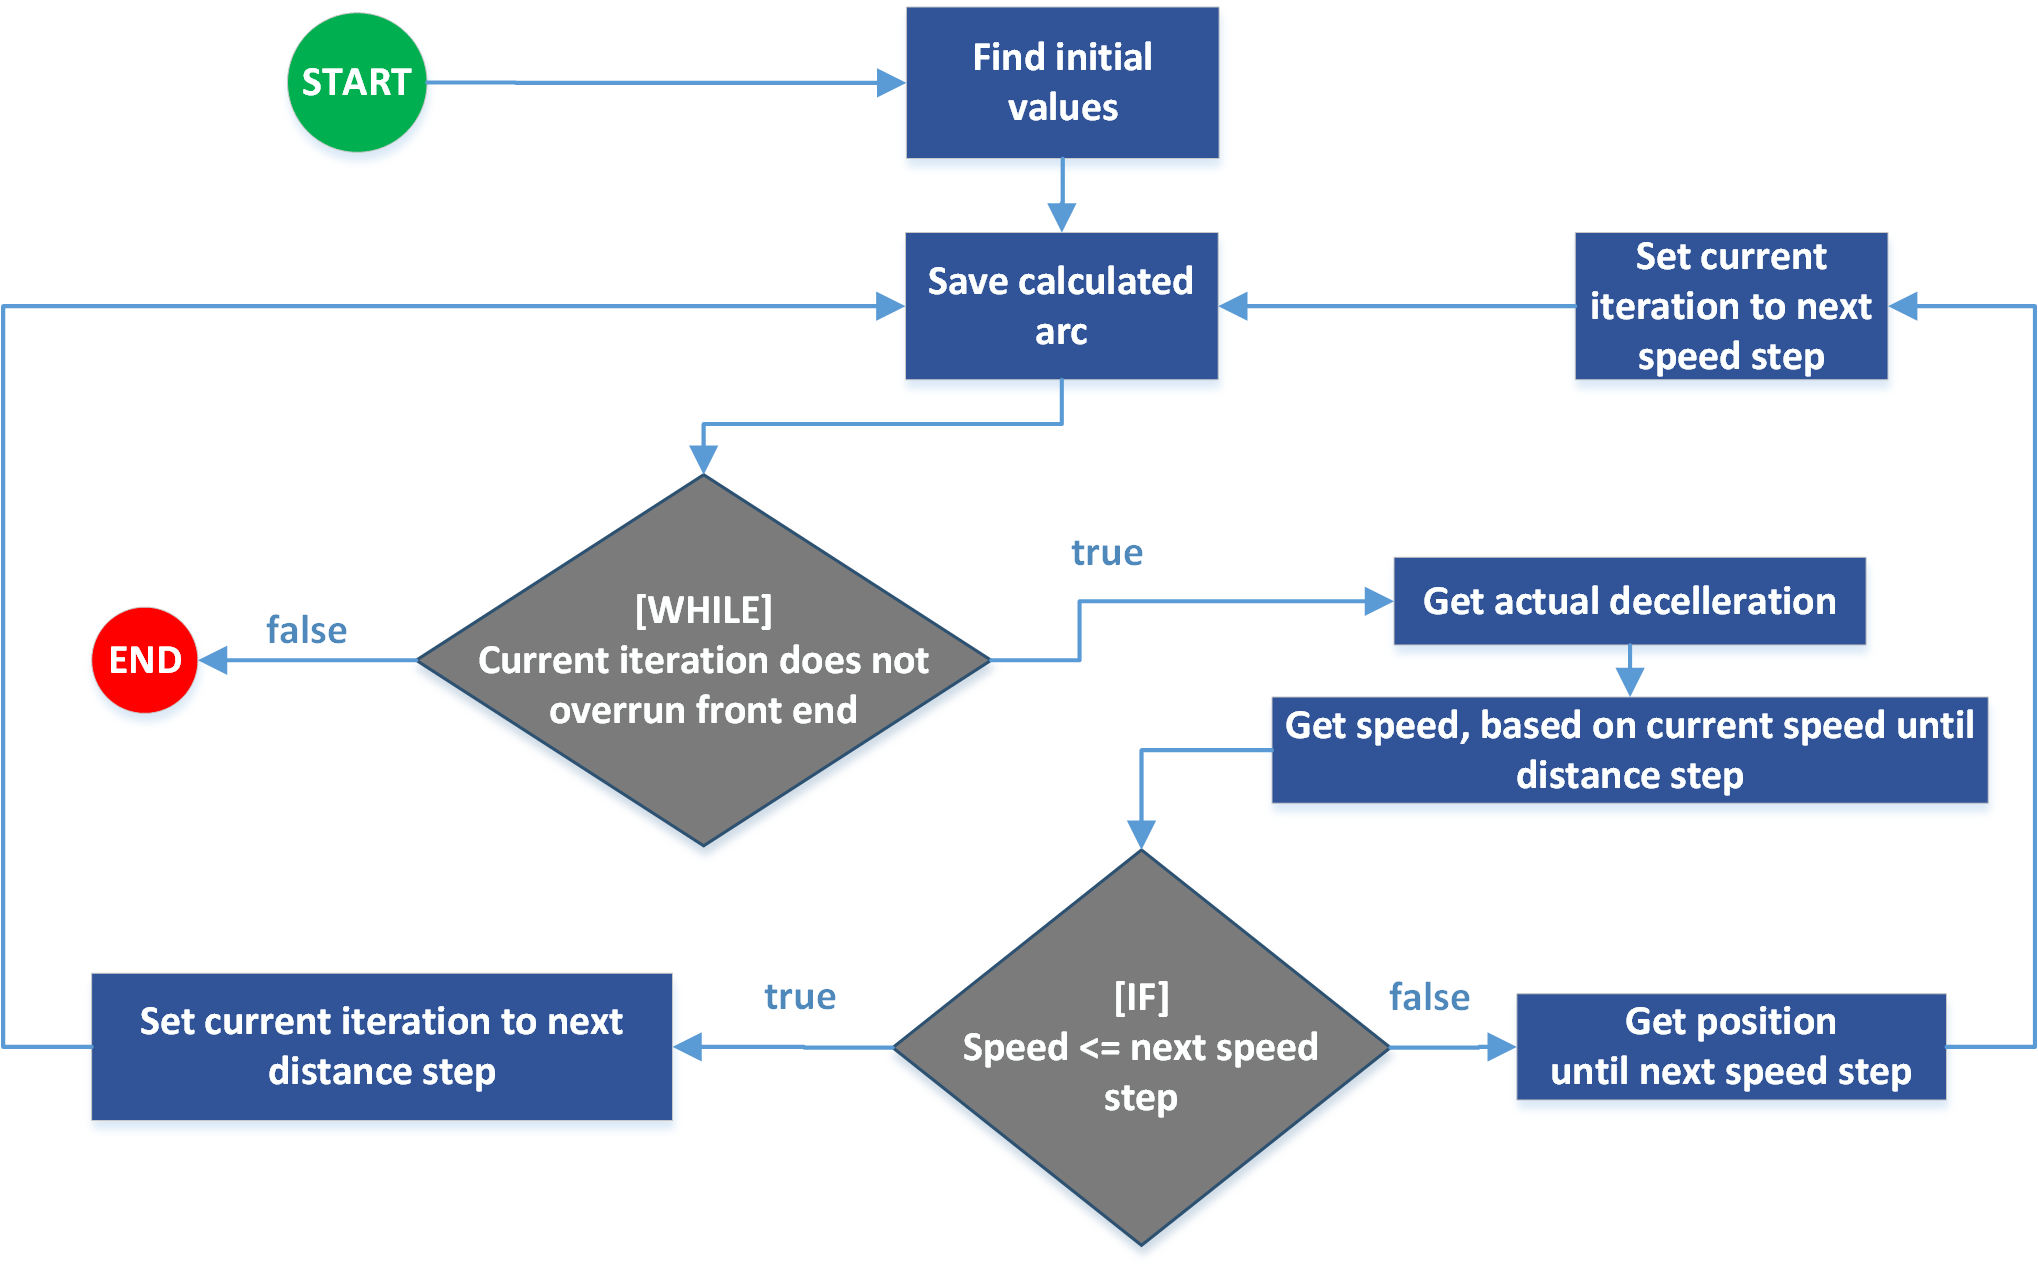
\includegraphics[width=0.95\textwidth]{../images/EBD_CalcAlgorithm.png}
\caption{Calculation of Braking Curves}\label{fig:bc_calc}
\end{figure}

Currently, the model supports the calculation of the following braking curves:
\begin{itemize}
	\item the Emergency Brake Deceleration curve for the most restrictive speed profile,
	%
	\item the Emergency Brake Deceleration curve for the limit of authority,
	%
	\item the Emergency Brake Deceleration curve for the end of authority, and
	%
	%\item the Service Brake Deceleration curve for the end of authority
\end{itemize}

\subsubsection{Reference to the Scade Model}

\subsection{SDMLimitLocations in Train Supervision}
\subsubsection{Reference to the SRS or other Requirements (or other requirements)}
\begin{itemize}
	\item \cite[Chapt.~3.13.9]{subset-026}: Supervision Limits 
	\item \cite[Chapt.~5.3.1.2]{subset-041}: $f_{41}$ -- accuracy of speed known on-board
	\item \cite[Chapt.~3.13.10]{subset-026}: Monitoring Commands as reference for required outputs of this module
\end{itemize}

\subsubsection{Short description of the functionality}
This operator calculates the various locations needed to determine the speed and distance monitoring commands. The current implementation of functionality is stateless and requires a complete recalculation each cycle.

\subsubsection{Interface}
\paragraph{Input}
\begin{enumerate}
  \item \texttt{MRSPProfile} Speed profile related to current track under train.
  \item \texttt{odometry}, \texttt{trainLocations} External state of train provided by odometry.
  \item \texttt{targetCollection} The different target (list) types wrapped in a structure.
  \item \texttt{curveCollection} The related braking curves correlated to above targets.
  \item \texttt{$v_{\mathit{release}}$} Release speed as defined by external sources.
  \item \texttt{$v_{mathit{ura}}$} Speed under reading amount.
  \item \texttt{inhibitUnderReadingCompensation} A flag defined by National Value, relating to above item.
  \item \texttt{$T_{bs}$, $T_{be}$, $T_{\mathit{tractionCutOff}}$} Time constants defined externally or in other modules.
\end{enumerate}
\paragraph{Output}
\begin{enumerate}
  \item \texttt{locations} Internal type to wrap the locations calculated herein and pass it on directly to SDM-Commands-Operator.
  \item \texttt{MostRestrictiveTarget} An internal structure to contain the information the target based locations are linked to.
  \item \texttt{FLOIisSBI1} Flag is true if First Line of Intervention uses the service brake curve (SBI1) or false if it uses deceleration values based on the emergency brake curve (SBI2).
  \item \texttt{$v_{\mathit{target}}$} The designated speed of the Most Restrictive Target. This is a convenience reference into the above data structure. 
  \item \texttt{$v_{mathit{MRSP}}$} The current Most Restrictive Speed at the Max Safe Frontend of the train.
\end{enumerate}

\subsubsection{Functional Design Description}
This operator gathers all necessary input values and computes some frequently used intermediate values in the operators \texttt{surplusTractionDeltas} and \texttt{$v_{\mathit{bec}}$}. The other input preparation operator is the \texttt{TargetSelector} whose main task is to dissect the list of targets to find the Most Restrictive Target. The accompanying braking curves are extracted and promoted to trailing location calculations. Also the special values of the EOA are exposed.

The operator creates the requested values for the commands package. These are in particular the preindication locations for EBD and SBD based targets, the release speed monitoring start locations, the locations for target speed monitoring of the I-, W-, P- and FLOI-curve, the related FLOI speed and the location of the permitted speed supervision limit. Included in the output are also certain flags for the validity of linked values.

%%\paragraph{Reference to the Scade Model}
%%\textbf{only in special case or link to the Scade model}

\subsection{CalcSpeeds in Train Supervision}

\subsubsection{Reference to the SRS or other Requirements (or other requirements)}
\begin{itemize}
	\item \cite[Chapt.~3.13.9]{subset-026}: Supervision Limits 
\end{itemize}

\subsubsection{Short description of the functionality}
This operator calculates the various speeds needed to determine the speed and distance monitoring commands.

\subsubsection{Interface}

\subsubsection{Functional Design Description}
This operator will be integrated into other operators in the next iteration.

%\paragraph{Reference to the Scade Model}
\textbf{only in special case or link to the Scade model}

\subsection{ReleaseSpeed\_Selection in Train Supervision}

\subsubsection{Reference to the SRS or other Requirements (or other requirements)}
\begin{itemize}
	\item \cite[Chapt.~3.8]{subset-026}: Movement authority 
\end{itemize}

\subsubsection{Short description of the functionality}
This operator outputs the release speed which can be given either by the national values or the movement authority.

\subsubsection{Interface}

\subsubsection{Functional Design Description}
This operator will be integrated into other operators in the next iteration.

\paragraph{Reference to the Scade Model}
%\textbf{only in special case or link to the Scade model}


\subsection{SDM\_Commands in Train Supervision}

\subsubsection{Reference to the SRS or other Requirements (or other requirements)}
\begin{itemize}
	\item \cite[Chapt.~3.13.10]{subset-026}: Speed and distance monitoring commands 
\end{itemize}

\subsubsection{Short description of the functionality}
This operator models the speed and distance monitoring commands. More precisely, it triggers the service or emergency brake and outputs the current supervision status of the OBU together with information on speeds and locations to the driver.

\subsubsection{Interface}

\subsubsection{Functional Design Description}
The OBU can be in any of three types of speed and distance monitoring modes: ceiling speed monitoring, release speed monitoring and target speed monitoring. We use a state machine to model the switching between the three modes: each state models a mode and a transition between to states is enabled if the condition two switch between the two corresponding modes is evaluated to true. In each mode, the OBU can be in up to five different supervision stati. The behavior of changing from one status to another is also modeled as a state machine. As a result, the model is a hierarchical state machine.

\subsubsection{Reference to the Scade Model}
%\textbf{only in special case or link to the Scade model}

\subsection{SDM\_OutputWrapper in Train Supervision}

\subsubsection{Reference to the SRS or other Requirements (or other requirements)}
\begin{itemize}
	\item \cite[Chapt.~3.13]{subset-026}: Speed and distance monitoring 
\end{itemize}

\subsubsection{Short description of the functionality}
This operator is the counterpart to operator SDM\_OutputWrapper---that is, it converts all internal outputs of block ``Speed Supervision'' that contain information about length, speed, distance, and acceleration defined as real into int, such that all other blocks can stick to their types and also performs the calculation into units used by the environment.

\subsubsection{Interface}

\subsubsection{Functional Design Description}
This operator forwards input messages and transforms inputs messages into an internal type thereby converting real to int.
  
\subsubsection{Reference to the Scade Model}
%\textbf{only in special case or link to the Scade model}%Mainfunction receive track data. Name should be be defined and substituded by the designer of the function. 

%-----------------------------------------------------------------------
\subsection{Manage ETCS Procedures}
%-----------------------------------------------------------------------
%\tbc
%Baseliyos Jacob

\subsubsection{Start of Mission - Awakness of Train}%Mainfunction receive track data. Name should be be defined and substituded by the designer of the function. 
\paragraph{Reference to the SRS or other Requirements (or other requirements)}
Chapter 5, § 5.4
\paragraph{Short descriptoiin of the functionality}
This functionality describes the Start of Mission procedure of the train until the status of the awakness. From this point of the awakness the train will be able to start different modes, levels and further procedure.
See scope of the Start of Mission - Awakness of train in the figure below.

\begin{figure}[h]
\centering
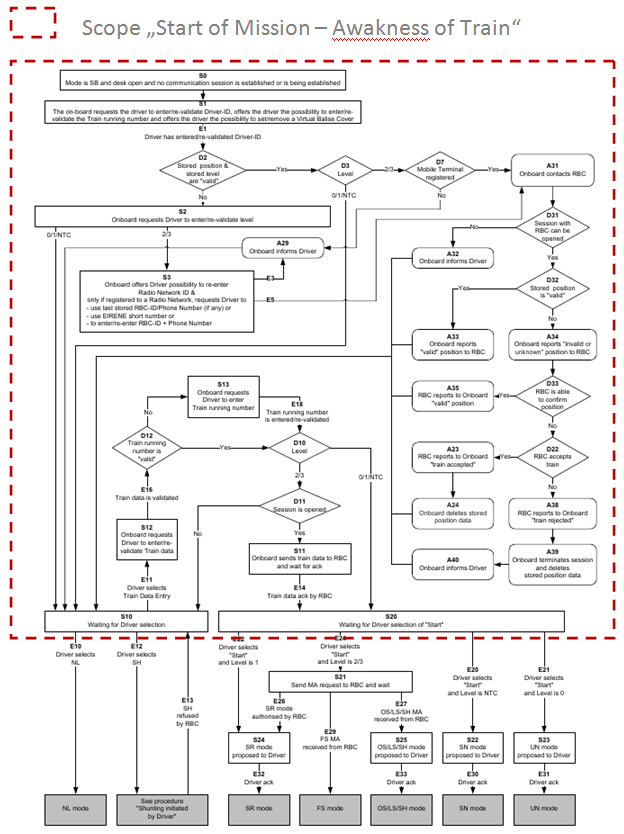
\includegraphics[scale=0.8]{images/SoMAwaknessoftrain}
\caption{Start of Mission - Awakness of Train}
\label{Start of Mission - Awakness of Train}
\end{figure}

\paragraph{Interface}
\textbf{Input Flow}
\begin{itemize}
\item Information from TIU
\item Action from Driver (DMI)
\item Information from Position Calculation
\item Information from Persistent Data
\item Information from Management of Radio Communication
\item Information from Mode and Level Management (Level and Mode Status)
\item Information from Radio Block Control
\end{itemize}

\textbf{Output Flow}
\begin{itemize}
\item Information to Management of Radio Communication
\item Request to Management of Radio Communication
\item Request to Driver (DMI)
\item Request to Mode and Level Management (Request Mode Change)
\item Request to Radio Block Control (Validation of Train Data)
\end{itemize}

\paragraph{Functional Design Description}
For the third iteration just a part of the Scope has been design. To complete the scenario in the third iteration the ideal path to the awakness of train until the state "waiting for Driver selection of "Start"" have been realized. Furthermore the initial data from the persistend database such as Level, Driver ID, Train Number, Train Data, Radio Number, RBC ID hase been consider as constants. 

\paragraph{Refernce to the Scade Model}
\url{https://github.com/openETCS/modeling/blob/master/model/Scade/System/ObuFunctions/Procedures/ManageProcedure_Pkg.xscade}

\subsubsection{Start of Mission in Level 2 or 3 Mode SR FS OS LS SH}
\paragraph{Reference to the SRS or other Requirements (or other requirements)}
Chapter 5, § 5.4
\paragraph{Short description of the functionality}
This functionality describes the Start of Mission procedure of the train in Level 2 or 3 and the Modes SR FS OS LS SH where the train under the defined Mode Level supervision starts running.
See scope of the Start of Mission - Level 2 or 3 and Modes SR FS OS LS SH in the figure below.
\begin{figure}[h]
\centering
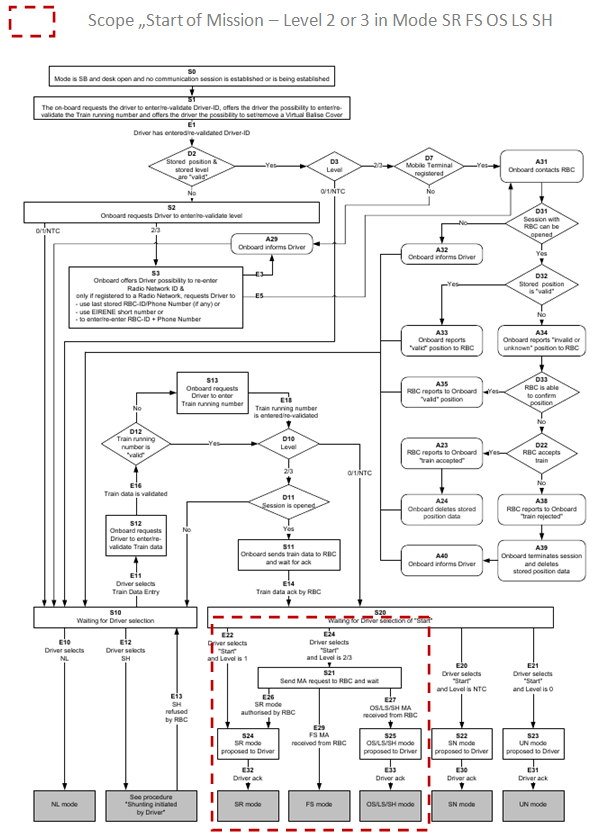
\includegraphics[scale=0.7]{images/SoMLevel2_3_SR_FS_OS_LS_SH}
\caption{Start of Mission - Start of Mission in Level 2 or 3 and Mode SR FS OS LS SH}
\label{Start of Mission - Start of Mission in Level 2 or 3 and Mode SR FS OS LS SH}
\end{figure}

\newpage

\paragraph{Interface}
\textbf{Input Flow}
\begin{itemize}
\item Action from Driver (DMI)
\item Information from Mode and Level Management (Level and Mode Status)
\item Information from Movement Authority Managmement (Receiving of Movement Authority)
\end{itemize}

\textbf{Output Flow}
\begin{itemize}
\item Request to Driver (DMI)
\item Request to Movement Authority Management (Request Movement Authority)
\item Request to Mode and Level Management (Request Mode Change)
\end{itemize}


\paragraph{Functional Design Description}
For the third iteration just a part of the Scope has been design. To complete the scenario in the third iteration the path "Full Supervision Movement Authority received from RBC" has been realized. The state will end after the train receives the Change Authority to FS and will be ready to run.

\paragraph{Refernce to the Scade Model}
\url{https://github.com/openETCS/modeling/blob/master/model/Scade/System/ObuFunctions/Procedures/SoM_SR_FS_OS_LS_SH_SN_UN.xscade}

%Mainfunction receive track data. Name should be be defined and substituded by the designer of the function. 

%-----------------------------------------------------------------------
\subsection{Manage Track Data}
%-----------------------------------------------------------------------
%\tbc
%Jakob Gärtner

\subsubsection{F.2.2 Calculate Train Position}\label{sss:calctrainpos}

\begin{itemize}
\item \textbf{Short Description of Functionality}\\
The main purpose of the function is to calculate the locations of linked and unlinked balise groups (BGs) and the current train position while the train is running along the track. 

\begin{figure}[hbtp]
\centering
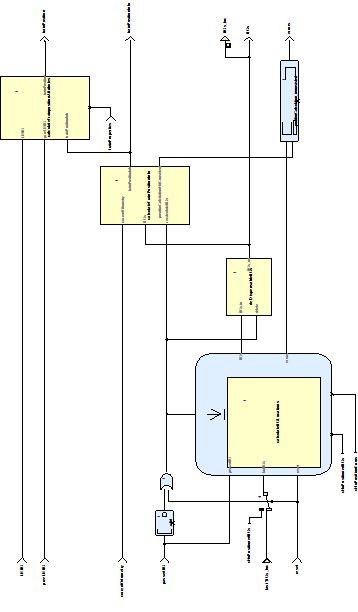
\includegraphics[scale=1]{../images/CalculateTrainPosition.png}
\caption{Structure of calculateTrainPosition}
\end{figure}


\paragraph{Functional Structure in Stages}
The whole function calculateTrainPosition is subdivided into the following steps, which are performed sequentially: 
\begin{enumerate}
\item \textbf{\textit{calculateBGLocations}}: Calculate the balise group locations\\
The first stage is triggered each time the train passes a balise group (input \textit{passedBG}). It takes the balise group header with the BG identification, the linking information (Subset 26, packet 5) and the current odometry values as inputs and calculates the location of the the passed balise group. If the passed BG has been announced via linking information previously, it takes into account the linking as well as the odometry information. If the passed BG does not meet the tolerance window announced by linking, an error flag is set. If the passed BG is an unlinked BG, its location is determined by odometry only, but related to the next previously passed linked BG, if there is one.\\
Then, if the passed BG is a linked BG comprising linking information for BGs ahead, the linking information is evaluated by creating the announced BGs and computing their locations from the linking distances.\\
The passed and the announced BGs are stored in a list \textit{BGs}, ordered by their nominal location on the track.\\
Afterwards the locations of all BGs are further improved by re-adjusting their locations with reference to the just passed BG. This optimizes the BG location inaccuries around the current train position (= location of the passed BG). 

\item \textbf{\textit{delDispensableBGs}}: Delete dispensable balise groups\\
The second stage removes balise groups supposed not to be needed any longer from the list of \textit{BGs}.\\
If the number of stored passed linked BGs exceeds the maximum number of eight as specified in subset-26-3.6.2.2.2 c), all BGs astern are deleted.
If only (passed) unlinked BGs are in the list and exceed the number of \textit{cNoOfAtLeast\_x\_unlinkedBGs}, all passed BGs astern to those are removed from the list. 

\item \textbf{\textit{calculateTrainPositionInfo}}: Calculate train position information.\\
This stage take the list of stored BGs and the current odometry values as inputs and steadily provides the current train position. 

\item \textbf{\textit{calculateTrainpositionAttributes}}: Calculate train position attribute information.\\
This stage provides several additional position related attributes that might conveniently be used by subsequent consumers in the architecture. It requires the actual LRBG and the previous LRBG to be assigned external from the list \textit{BGs}. 

\end{enumerate}

\item \textbf{Reference to the SRS (or other requirements)}\\
\\
The component calculateTrainPosition determines the location of linked and unlinked balise groups and the current train position during the train trip as specified mainly in subset-026-3.6

\item \textbf{Design Constraints and Choices}\\
\\
The following constraints and prerequisites apply:

\begin{enumerate}
\item The input data received from the balises groups must have been checked and filtered for validity, consistency and the appropriate train orientation before delivering them to calculateTrainPosition. 
\item The storage capacity for balise groups is finite. calculateTrainPosition will raise an error flag when a balise group cannot be stored due to capacity limitations.
\item calculateTrainPosition will raise an error flag if a just passed balise group is not found where announced by linking information. It will not (yet) detect when an announced balise group is missing. 
\item calculateTrainPosition is not yet prepared for train movement direction changes. 
\item calculateTrainPosition does not yet consider repositioning information.
\end{enumerate}

\end{itemize}

\subsubsection{Provide Position Report}\label{sss:provposrep}

\begin{figure}[ht]
\centering
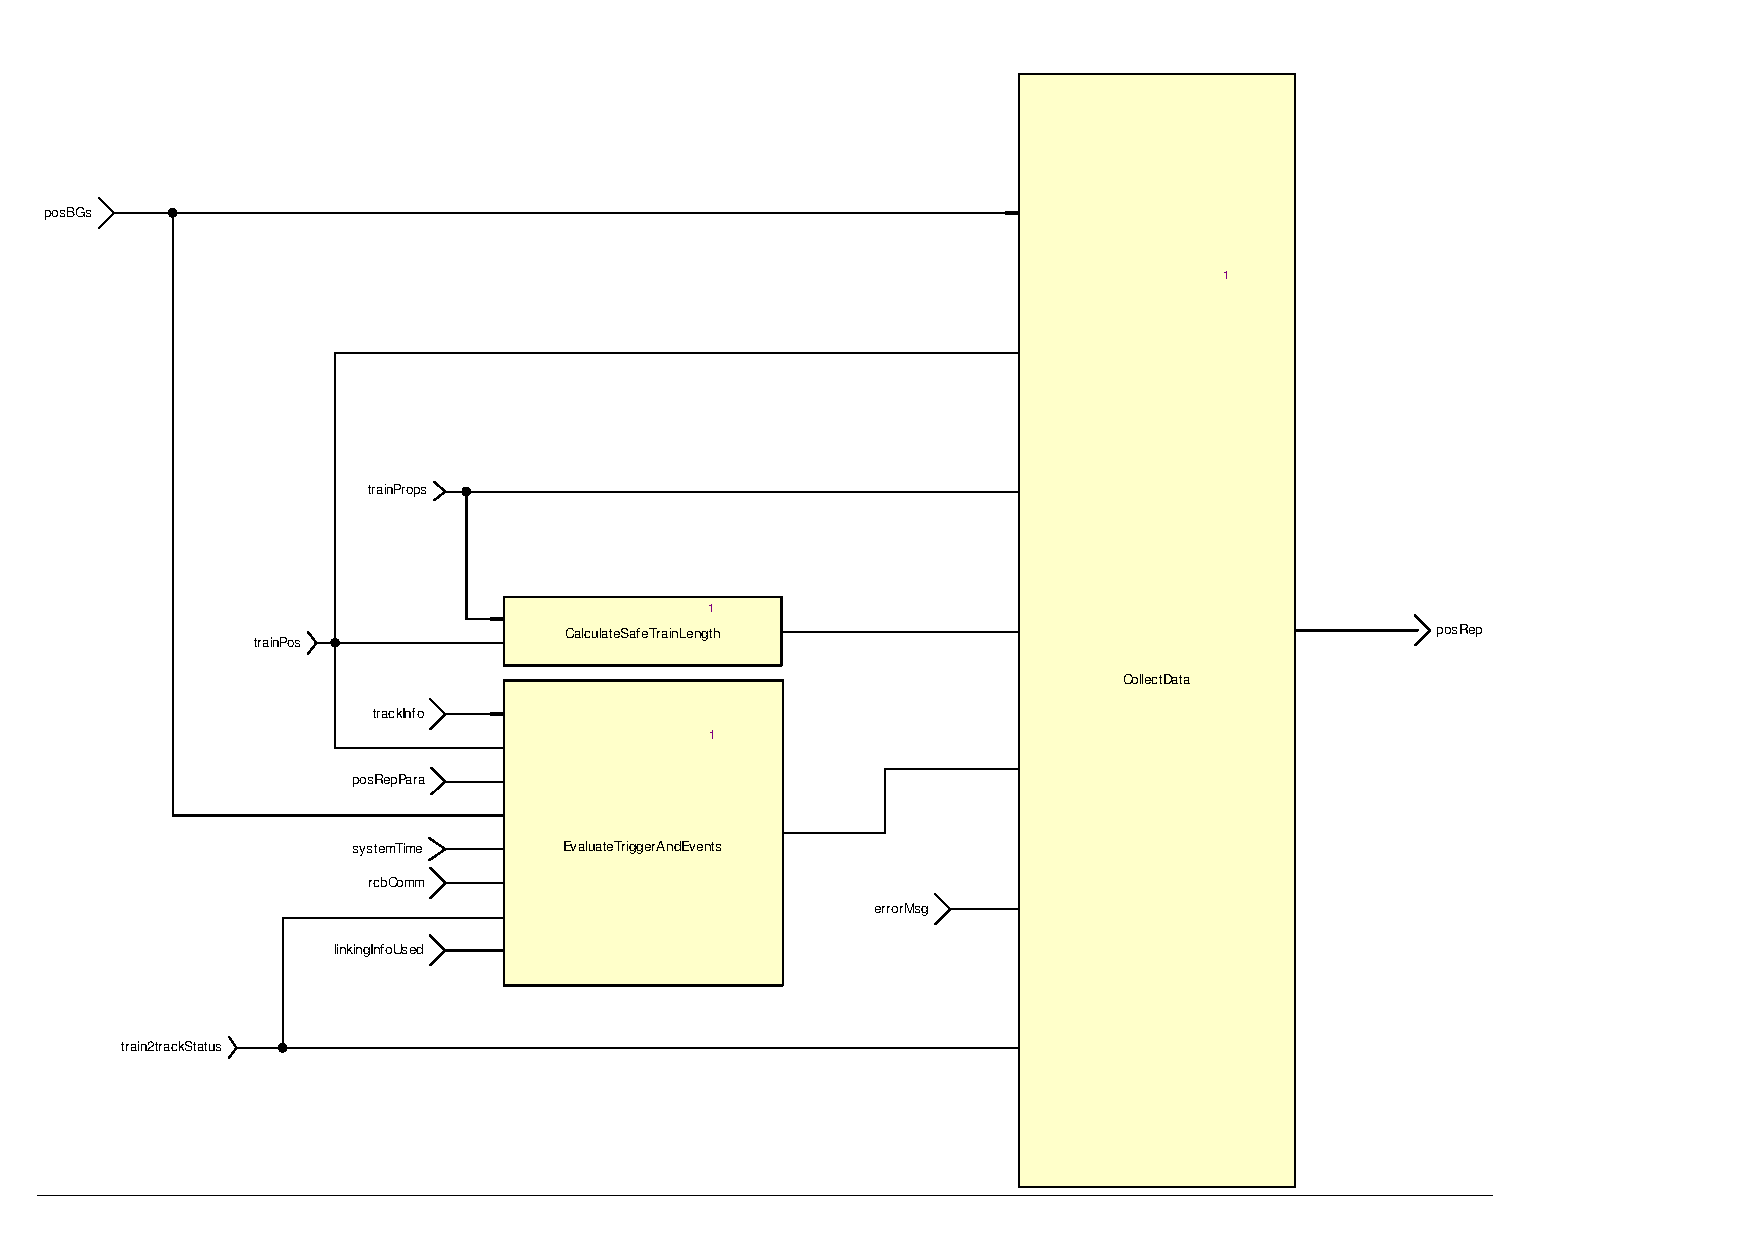
\includegraphics[scale=0.6]{../images/ProvidePositionReport.pdf}
\caption{Structure of component ProvidePositionReport}\label{fig:provideposrep}
\end{figure}

\begin{itemize}
\item \textbf{Short Description of Functionality}\\
This function takes the current train position and generates a position report which is sent to the RBC. The point in time when such a report is sent is determined from event, on the one hand, and position report parameters---which are basically triggers---provided by the RBC or a balise group passed, on the other hand. The functionality is modeled using three operations, as shown in Fig.~\ref{fig:provideposrep}, which are explained below.
\begin{description}
	\item[CalculateSafeTrainLength] Calculates the the safeTrainLength according to Chapt.~3.6.5.2.4/5.
\verb+safeTrainLength = absolute(EstimatedFrontEndPosition - MinSafeRearEnd)+, where
\verb+MinSafeRearEnd = minSafeFrontEndPosition - L_TRAIN+
	\item[EvaluateTriggerAndEvents] Returns a Boolean modeling whether the sending of the next position report is triggered or not. It is the conjunction of the evaluation of all triggers (PositionReportParameters, i.e., Packet 58) and events (see Chapt.~3.6.5.1.4).
	\item[CollectData] In this operation, data of Packet0, \dots, Packet5 and the header is aggregated to a position report.
\end{description}
\item \textbf{Reference to the SRS (or other requirements}\\
Most of the functionality is described in subset 26, chapter~3.6.5.
\item \textbf{Design Constrains and Choices}\\
\begin{enumerate}
	\item The message length (i.e., attribute \verb+L_MESSAGE+) is by default set to 0; the actual value will be set by the Bitwalker/API.
	\item The attribute \verb+Q_SCALE+ is assumed to be constant; that is, all operations using this attribute do not convert between different values of that attribute.
	\item \textit{PositionReportHeader}: The time stamp (i.e., attribute \verb+T_TRAIN+) is not set; this should be done once the message is being sent by the API
	\item \textit{Packet4}: When aggregating the data for this packet, an error message might be overwritten by a succeeding error message. Because the specification only allows to sent one error in one position report, errors are not being stored in a queue, for instance.
	\item \textit{Packet44}: This packet is currently not contained in a position report as it is not part of the kernel functions.
	\item The usage of attributes \verb+D_CYCLOC+ and \verb+T_CYCLOC+ as part of the triggers specified by the position report parameters (i.e., Packet 58 sent by the RBC) may lead to unexpected results if a big clock cycle together with small values for the attributes is used. The cause is that the current model increments at every clock cycle the reference value for the distance and time by at most \verb+D_CYCLOC+ and \verb+T_CYCLOC+, respectively and not a factor of it.
\end{enumerate}
\item \textbf{Open Issues}
\begin{enumerate}
	\item Operation \textit{EvaluateTriggerAndEvents} currently ignores parameters \verb+N_ITER+, \verb+D_LOC+ and \verb+D_LGTLOC+ which allow to specify up to 32 position at which a report has to be sent. The positions are relative to the location of a reference balise group. If the RBC sends packet 58, then it also provides a reference balise group; otherwise, if packet 58 is sent by a balise group, then this balise group serves a the reference balise group. Possible realisation in the model: Extend in the interface posRepPara (i.e., Packet 58) by a \verb+NID_BG+ referring to the reference balise group. Am assumption would be that this BG can be found in the list of passed balise group provided by \textit{CalculateTrainPosition} in Sect.~\ref{sss:calctrainpos}.
	\item The specification requires to store the last eight balise groups for which a position report has been sent (see 3.6.2.2.2.c).
	\item For all reports that contain Packet 1 (i.e., report based on two balise groups), the RBC sends a coordinate system. It is unclear where this has to be stored (i.e., somehow the balise groups have to be stored in a database which has then to be updated), see 3.4.2.3.3.6. Moreover, such a coordination system can be invalid and then has to be rejected (see 3.4.2.3.3.7-8). On a more abstract level, we need to think about the interface between the RBC and the OBU or a proper abstraction thereof.
	\item The decision whether a the report consists of packet 0 or packet 1, which is provided in 3.4.2.3.3, is currently not completely modeled. So far, 3.4.2.3.3.1 has only been modeled, thereby assuming ``the last balise group detected'' is the last balise group and not the LRBG. 3.4.2.3.3.2 is unclear. To model 3.4.2.3.3.4 I need information about the last two valid balise groups and the train running direction. This information can be obtained by adding a memory or this information will be provided by \textit{CalculateTrainPosition} in Sect.~\ref{sss:calctrainpos}. Likewise, also 3.4.2.3.3.5 requires knowledge about the last two valid balise groups.
\end{enumerate}
\end{itemize}
 


%\subsubsection{functional block x in Manage Track Data}%MainfunctionManage Track Data.. Name should be be defined and substituded by the designer of the function. 
%\paragraph{Reference to the SRS or other Requirements (or other requirements)}
%\paragraph{Short descriptoiin of the functionality}
%\paragraph{Interface}
%\paragraph{Functional Design Description}
%\paragraph{Refernce to the Scade Model}
%\textbf{only in special case or link to the Scade model}

%\subsubsection{functional block x in Manage Track Data}%Mainfunction Manage Track Data. Name should be be defined and substituded by the designer of the function. 
%\paragraph{Reference to the SRS or other Requirements (or other requirements)}
%\paragraph{Short descriptoiin of the functionality}
%\paragraph{Interface}
%\paragraph{Functional Design Description}
%\paragraph{Refernce to the Scade Model}
%\textbf{only in special case or link to the Scade model}

%\subsubsection{functional block x in Manage Track Data}%Mainfunction Manage Track Data. Name should be be defined and substituded by the designer of the function. 
%\paragraph{Reference to the SRS or other Requirements (or other requirements)}
%\paragraph{Short descriptoiin of the functionality}
%\paragraph{Interface}
%\paragraph{Functional Design Description}
%\paragraph{Refernce to the Scade Model}
%\textbf{only in special case or link to the Scade model}

%\subsubsection{functional block x in Manage Track Data}%Mainfunction Manage Track Data. Name should be be defined and substituded by the designer of the function. 
%\paragraph{Reference to the SRS or other Requirements (or other requirements)}
%\paragraph{Short descriptoiin of the functionality}
%\paragraph{Interface}
%\paragraph{Functional Design Description}
%\paragraph{Refernce to the Scade Model}
%\textbf{only in special case or link to the Scade model} 

%Mainfunction receive track data. Name should be be defined and substituded by the designer of the function. 

%-----------------------------------------------------------------------
\subsection{Manage Data}
%-----------------------------------------------------------------------
%\tbc
%Group2 (Bernd Hekele)

\subsubsection{Macrofunction x in Manage Data}%Mainfunction Manage Data. Name should be be defined and substituded by the designer of the function. 
\paragraph{Reference to the SRS or other Requirements (or other requirements)}
\paragraph{Short descriptoiin of the functionality}
\paragraph{Interface}
\paragraph{Functional Design Description}
\paragraph{Refernce to the Scade Model}
\textbf{only in special case or link to the Scade model}

\subsubsection{Macrofunction x in Manage Data}%Mainfunction Manage Data. Name should be be defined and substituded by the designer of the function. 
\paragraph{Reference to the SRS or other Requirements (or other requirements)}
\paragraph{Short descriptoiin of the functionality}
\paragraph{Interface}
\paragraph{Functional Design Description}
\paragraph{Refernce to the Scade Model}
\textbf{only in special case or link to the Scade model}

\subsubsection{Macrofunction x in Manage Data}%Mainfunction Manage Data. Name should be be defined and substituded by the designer of the function. 
\paragraph{Reference to the SRS or other Requirements (or other requirements)}
\paragraph{Short descriptoiin of the functionality}
\paragraph{Interface}
\paragraph{Functional Design Description}
\paragraph{Refernce to the Scade Model}
\textbf{only in special case or link to the Scade model}

\subsubsection{Macrofunction x in Manage Data}%Mainfunction Manage Data. Name should be be defined and substituded by the designer of the function. 
\paragraph{Reference to the SRS or other Requirements (or other requirements)}
\paragraph{Short descriptoiin of the functionality}
\paragraph{Interface}
\paragraph{Functional Design Description}
\paragraph{Refernce to the Scade Model}
\textbf{only in special case or link to the Scade model}

%Mainfunction receive track data. Name should be be defined and substituded by the designer of the function. 

%-----------------------------------------------------------------------
\subsection{Manage Outputs}
%-----------------------------------------------------------------------
%\tbc
%Bernd Hekele

\subsubsection{Macrofunction x in Manage Outputs}%Mainfunction Manage Outputs. Name should be be defined and substituded by the designer of the function. 
\paragraph{Reference to the SRS or other Requirements (or other requirements)}
\paragraph{Short descriptoiin of the functionality}
\paragraph{Interface}
\paragraph{Functional Design Description}
\paragraph{Refernce to the Scade Model}
\textbf{only in special case or link to the Scade model}

\subsubsection{Macrofunction x in Manage Outputs}%Mainfunction Manage Outputs. Name should be be defined and substituded by the designer of the function. 
\paragraph{Reference to the SRS or other Requirements (or other requirements)}
\paragraph{Short descriptoiin of the functionality}
\paragraph{Interface}
\paragraph{Functional Design Description}
\paragraph{Refernce to the Scade Model}
\textbf{only in special case or link to the Scade model}

\subsubsection{Macrofunction x in Manage Outputs}%Mainfunction Manage Outputs. Name should be be defined and substituded by the designer of the function. 
\paragraph{Reference to the SRS or other Requirements (or other requirements)}
\paragraph{Short descriptoiin of the functionality}
\paragraph{Interface}
\paragraph{Functional Design Description}
\paragraph{Refernce to the Scade Model}
\textbf{only in special case or link to the Scade model}

\subsubsection{Macrofunction x in Manage Outputs}%Mainfunction Manage Outputs. Name should be be defined and substituded by the designer of the function. 
\paragraph{Reference to the SRS or other Requirements (or other requirements)}
\paragraph{Short descriptoiin of the functionality}
\paragraph{Interface}
\paragraph{Functional Design Description}
\paragraph{Refernce to the Scade Model}
\textbf{only in special case or link to the Scade model}

%Mainfunction receive track data. Name should be be defined and substituded by the designer of the function. 

%-----------------------------------------------------------------------
\subsection{Mode and Level}
%-----------------------------------------------------------------------
%\tbc
%Marielle Petit


The "Management of Modes and Levels" function is mainly described in chapter 4
and 5 of \citep{subset-026}. Modes and levels define the status of the ETCS
regarding on-board functional status and track infrastructure.

\begin{landscape}
\begin{figure}[hbtp]
\centering
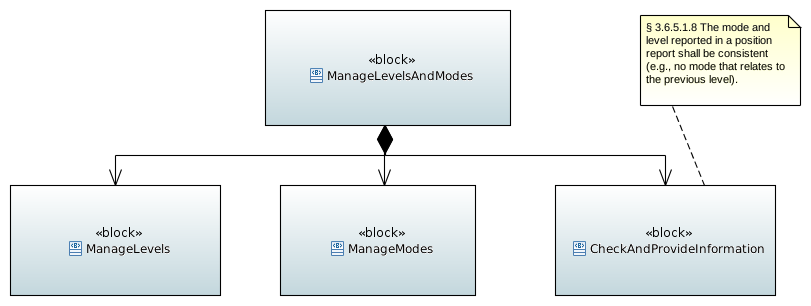
\includegraphics[scale=1]{images/FunctionalArchitecture.png}
\caption{High level Architecture}
\end{figure}
\end{landscape}

\subsubsection{Function Level Management}%Mainfunction receive track data. Name should be be defined and substituded by the designer of the function.
\paragraph{Reference to the SRS or other Requirements}

see \citep{subset-026} section 5.10

\paragraph{Short description of the functionality}

The level management subsystem receives level transition order tables and selects the order with the highest probability. It stores the information about the selected transition order and transits to the requested level once the train passes the location of the level transition.

If required, the driver is asked to acknowledge the transition, in case of no acknowledge or if conditions for the level transition are not fulfilled, the train gets tripped.

\paragraph{Interface}

The interface consists of the following inputs:

\begin{itemize}
\item \emph{conditional transitions:} a priority table containing the
  conditional level transition orders (from paquet 46)
\item \emph{level transition priority table:} a priority table containing the
  (non-conditional) level transition orders (from paquet 41)
\item \emph{train standstill:} a Boolean value indicating whether the train is
  at standstill (from odometry)
\item \emph{driver level transition:} a level transition order selected by the
  driver (from DMI)
\item \emph{ERTMS capabilities:} the ERTMS capabilities of the track
\item \emph{getAck:} Boolean input that signals the acknowledgment of the
  driver (from DMI)
\item \emph{resetIdle:} Boolean input to reset without acknowledge
\item \emph{currentDistance:} the current position of the train given with the
  same reference as the position of the level transition order (train position , from localisation)
\item \emph{ackDistance:} the maximal distance for driver acknowledge after
  the level transition (from paquet 41)
\item \emph{immediateAck:} a Boolean that signals that an immediate acknowledge
  is required
\item \emph{received L2 L3 MA:} a Boolean that indicates that a level 2 or level
  3 movement authority for the track behind the level transition has been
  received (from paquet 15)
\item \emph{received L1 MA:} a Boolean that indicates that a level 1 movement
  authority for the track behind the level transition has been received (from paquet 12)
\item \emph{received target speed:} a Boolean indicating that a target speed for
  the track behind the level transition has been received (from paquet 27) ?
\end{itemize}

and the following outputs:

\begin{itemize}
\item \emph{next level:} the next level after this computation cycle
\item \emph{Trip train:} a Boolean indicating whether the train should be
  tripped
\item \emph{previous level:} the previous level before this computation cycle
\item \emph{needsAckFromDriver:} a Boolean that indicates whether an
  acknowledgment from the driver is necessary
\end{itemize}

\paragraph{Functional Design Description}

On the most abstract level the design consists of the \emph{manage\_priorities} function which takes the level transition order priority tables as inputs and computes the highest priority transition.

This transition order is the fed to the \emph{computeLevelTransitions} operator. This operator consists of three main parts. The \emph{ComputeTransitionConditions} operator that emits the fulfilled conditions to change from a given level to a new level, the \emph{LevelStateMachine} that stores the current level and takes the computed change conditions as input for possible level transitions and finally the \emph{driverAck} operator which contains a state machine that stores the information whether the system is currently waiting for a driver acknowledge and emits the train trip information if necessary.


\paragraph{Reference to the Scade Model}

The Scade model is available on github:
\url{https://github.com/openETCS/modeling/tree/master/openETCS ArchitectureAndDesign/Work Groups/Group 3/SCADE/LevelManagement/}

%%%%%%%%%%%%%%%%%%%%%%%%%%%%%%%%%%%%%%%%%%%%%%%%%%%%

\subsubsection{Function Mode Management}%Mainfunction receive track data. Name should be be defined and substituded by the designer of the function.
\paragraph{Reference to the SRS or other Requirements}
see \citep{subset-026} sections 4.4, 4.6, 5.4, 5.5, 5.6, 5.7, 5.8, 5.9, 5.11, 5.12, 5.13, 5.19

\paragraph{Short description of the functionality}


This function is in charge of the computation of new mode to apply according to conditions from inputs (track information, driver interactions, train data,...) and other functions.

\paragraph{Interface}

The inputs are the following:
\begin{itemize}
\item \emph{Cab} identification of the current cabin (A or B)
\item \emph{Continue\_shunting\_Function\_Active}: boolean to describe the activation state of the shunting function
\item \emph{Current\_Level}: outputs of the Level management function
\item \emph{Data\_From\_DMI}: set of data received from the driver via the DMI interface, indeed:
\begin{itemize}
\item \emph{Ack\_LS : bool} Driver acknoledges LS mode
\item \emph{Ack\_OS : bool}
\item \emph{Ack\_RV : bool}
\item \emph{Ack\_SH : bool}
\item \emph{Ack\_SN : bool}
\item \emph{Ack\_SR : bool}
\item \emph{Ack\_TR : bool}
\item \emph{Ack\_UN : bool}
\item \emph{Req\_Exit\_SH : bool} driver selects exit of shunting
\item \emph{Req\_NL : bool} Driver requests NL mode
\item \emph{Req\_Override : bool} Driver requests override function
\item \emph{Req\_SH : bool} driver requests SH mode
\item \emph{Req\_Start : bool} Driver requests start of mission
\item \emph{ETCS\_Isolated: bool}: isolation status of the ETCS
\end{itemize}
\item \emph{Data\_From\_Localisstion}: set of data received from the function in charge of localistion of the train, indeed:
\begin{itemize}
\item \emph{BG\_In\_List\_Expected\_BG\_In\_SR : bool}: the identity of the overpass balise group is in the list of expected balises related to SR mode (from SR to trip mode condition 36)
\item \emph{BG\_In\_List\_Expected\_BG\_In\_SH : bool}: the identity of the overpass balise group is in the list of expected balises related to SH mode (from SH to trip mode condition 52)
\item \emph{Linked\_BG\_In\_Wrong\_Direction : bool} balise group contained in the linking information is passed in the unexpected direction (from FS, LS, OS to trip mode condition 66) \emph{Localisaion function ?}
\item \emph{Train\_Position}: output provided by function in charge of computation of train possition (type	TrainPosition\_Types\_Pck::trainPosition\_T)	\item \emph{Train\_Speed : Obu\_BasicTypes\_Pkg::Speed\_T} provided by odometry function
\item \emph{Train\_Standstill : bool} provided by odometry function
\end{itemize}
\item \emph{Data\_From\_Speed\_and\_Supervision}: set of data received from the function in charge of speed and supervision management, indeed:
\begin{itemize}
\item \emph{Estim\_front\_End\_overpass\_SR\_Dist : bool}: the train overpass the SR distance with its estimated front end (from SR to trip mode condition 42) 
\item \emph{Estim\_Front\_End\_Rear\_SSP : bool}: estimated front end is rear of the start location of either SSP or gradient profile stored on-board (from FS, LS, OS to trip mode condition 69)
\item \emph{Override\_Function\_Active}: boolean to indicate the state of the activation function 	  	
\item \emph{EOA\_Antenna\_Overpass : bool}: the train overpasses the  EOA  with min safe antenna position Level 1 (from FS, LS, OS to trip mode condition 12)
\item \emph{EOA\_Front\_End : bool} the train overpasses the  EOA  with min safe front end, Level 2 or 3 (from FS, LS, OS to trip mode condition 16)
\item \emph{Train\_Speed\_Under\_Overide\_Limit : bool} supervision when override function is active (to SR mode condition 37)
\end{itemize}
\item \emph{Data\_From\_TIU : TIU\_Types\_Pkg::Message\_Train\_Interface\_to\_EVC\_T}:message provided by TIU interface
\item \emph{Data\_From\_Track}: set of data received from track side (via RBC or Balises telegram), indeed:
\begin{itemize}
\item \emph{MA\_SSP\_Gradiant\_Available : bool} MA, SSP and gradient have been received, checked and stored on-board from paquet 12, 15, 21 and 27 or message 3 or 33
\item \emph{Mode\_Profile\_On\_Board : Level\_And\_Mode\_Types\_Pkg::T\_Mode\_Profile} from packet 80
\item \emph{Shunting\_granted\_By\_RBC : bool} from message 27 and 28
\item \emph{Trip\_Order\_Given\_By\_Balise : bool}
\item \emph{List\_Bg\_Related\_To\_SR\_Empty : bool} from packet 63
\item \emph{Stop\_If\_In\_shunting : bool} from packet 135
\item \emph{Stop\_If\_In\_SR : bool} from packet 137
\item \emph{Error\_BG\_System\_Version : bool}
\item \emph{Linking\_Reaction\_To\_Trip : bool}
\item \emph{RBC\_Ack\_TR\_EB\_Revocked : bool} from message 6
\item \emph{RBC\_Authorized\_SR : bool} from message 2
\item \emph{Reversing\_Data : Level\_And\_Mode\_Types\_Pkg::T\_Reversing\_Data} from packet 138/ 139
\item \emph{T\_NVCONTACT\_Overpass : bool} Maximal time without new safe message overpass
\item \emph{Emergency\_Stop\_Message\_Received}: boolean to describe the reception of Emergency Stop message  from message 15 or 16
\end{itemize}
\item \emph{Failure\_Occured}: boolean to indicate safety failure occurence	
\item \emph{Interface\_To\_National\_System}: boolean to indicate existance of an interface to a national system 	  	
\item \emph{National\_Trip\_Order}: boolean to indicate reception of a trip order from a national system 	  	
\item \emph{OnBoard\_Powered}: boolean to indicate the poxering state of the system 	  	
\item \emph{Stop\_Shunting\_Stored}: boolean to store the information in regards of shunting function	  	
\item \emph{Valid\_Train\_Data\_Stored}: boolean to indication train data are available and valid.
\end{itemize}

The outputs are the following:

\begin{itemize}
\item \emph{currentMode} the new computed mode (typeis  Level\_And\_Mode\_Types\_Pkg::T\_Mode, default value is Level\_And\_Mode\_Types\_Pkg::SB )
\item \emph{EB\_Requested} boolean to request triggering of emergency brake 	  	
\item \emph{Service\_Brake\_Command} boolean to request command of service brake 	  	
\item \emph{Data\_To\_DMI}: set of data provided to the DMI	Level\_And\_Mode\_Types\_Pkg::T\_Data\_To\_DMI 	:  	
\begin{itemize}
\item \emph{Ack\_LS : bool} Driver acknoledges LS mode
\item \emph{Ack\_OS : bool}
\item \emph{Ack\_RV : bool}
\item \emph{Ack\_SH : bool}
\item \emph{Ack\_SN : bool}
\item \emph{Ack\_SR : bool}
\item \emph{Ack\_TR : bool}
\item \emph{Ack\_UN : bool}
\item \emph{Req\_Exit\_SH : bool} driver selects exit of shunting
\item \emph{Req\_NL : bool} Driver requests NL mode
\item \emph{Req\_Override : bool} Driver requests override function
\item \emph{Req\_SH : bool} driver requests SH mode
\item \emph{Req\_Start : bool} Driver requests start of mission
\item \emph{ETCS\_Isolated: bool}: isolation status of the ETCS
\end{itemize}
\item \emph{Data\_To\_BG\_Management}: set of date to trackside Level\_And\_Mode\_Types\_Pkg::T\_Data\_To\_BG\_Management 	: 
\begin{itemize}
\item \emph{EoM\_Procedure\_req : bool} request of end of mission procedure indeed end of the communication session for message 150
\item \emph{Clean\_BG\_List\_SH\_Area : bool} request to clean the BG  list when entering  an SH area §5.6.2
\item \emph{MA\_Req : bool} for message 132
\item \emph{Req\_for\_SH\_from\_driver : bool} for message 130
\end{itemize}
\end{itemize}

\paragraph{Functional Design Description}


Three subfunctions are defined:
\begin{description}
\item[Inputs] proceeds to inputs check and preparation.
\item[ComputeModesCondition] performs all specific procedure linked to mode management and defined in  \citep{subset-026} sections 5.4, 5.5, 5.6, 5.7, 5.8, 5.9, 5.11, 5.12, 5.13, 5.19 and specifies the conditions to define a mode transition according condition table of section 4.6.3 of \citep{subset-026}
\item[SwitchModes] performs the mode selection according the conditions and priorities defined in transition table  section 4.6.2 of \citep{subset-026}
\item[Outputs] prepares paquet of outputs.
\end{description}


\begin{landscape}
\begin{figure}[hbtp]
\centering
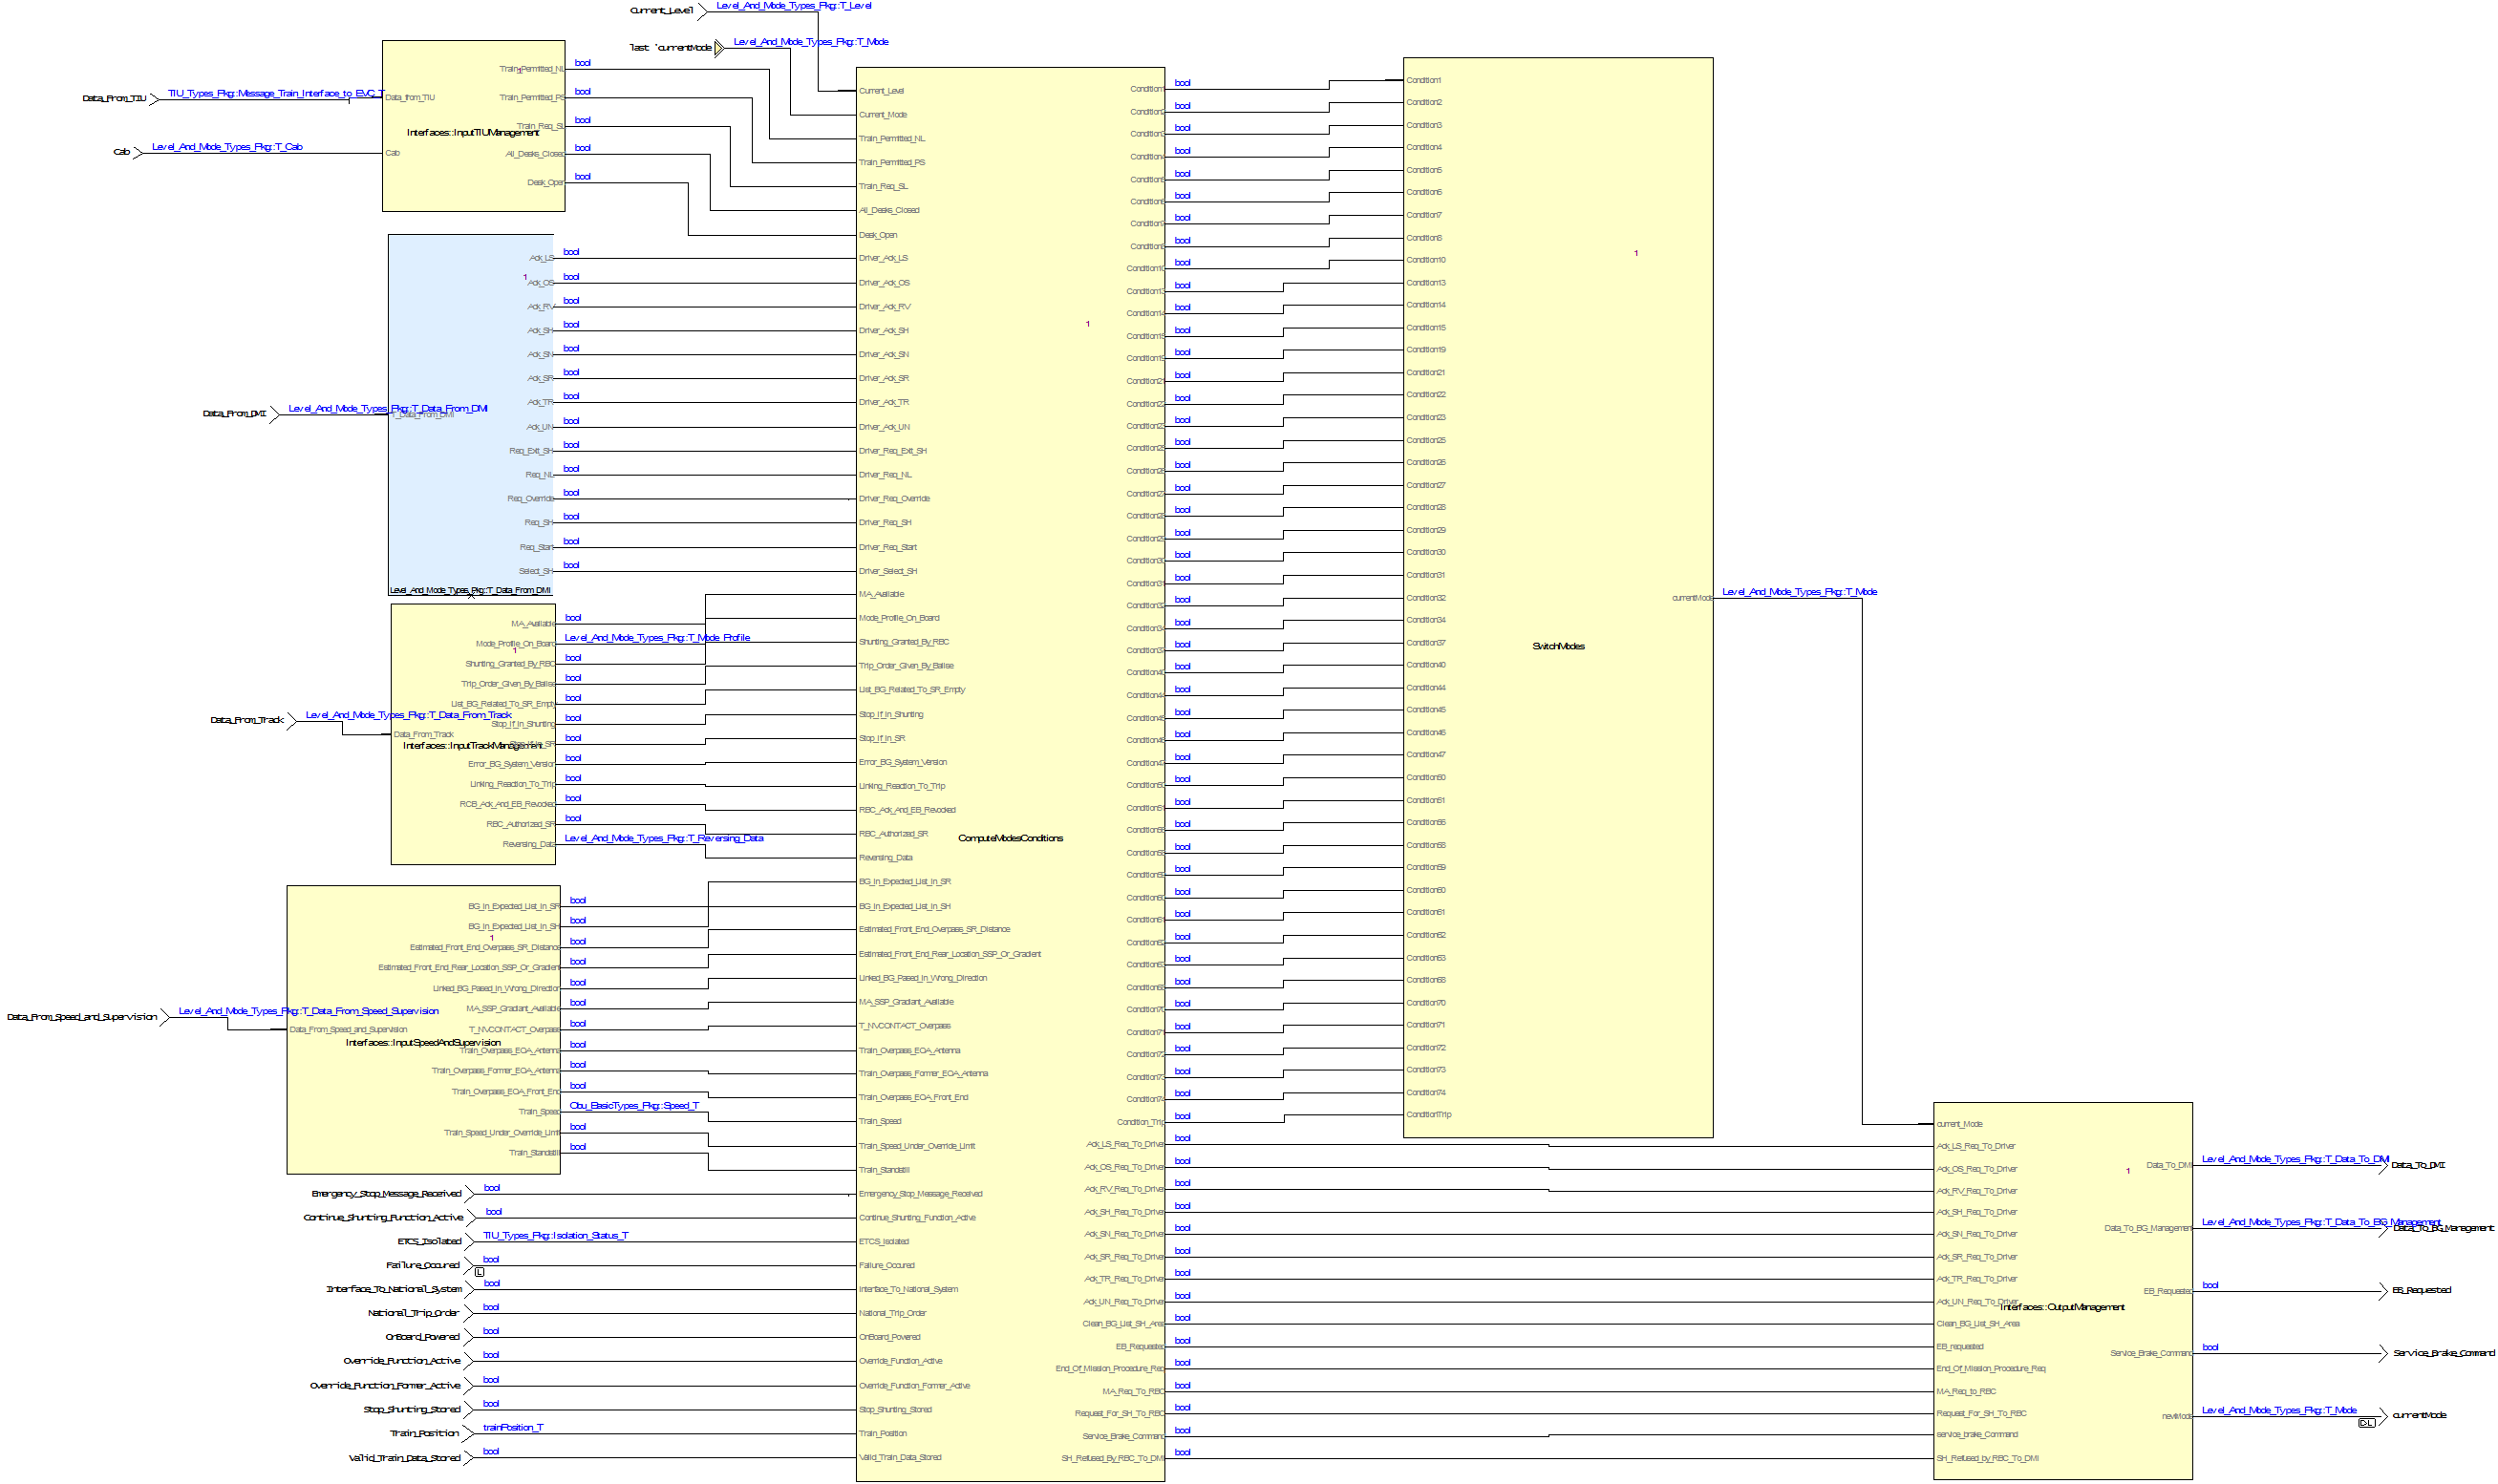
\includegraphics[scale=0.3]{images/ManageModes.png}
\caption{Modes subfubction architecture}
\end{figure}
\end{landscape}

\paragraph{Reference to the Scade Model}
The Scade model is available on github:
\url{https://github.com/openETCS/modeling/tree/master/model/Scade/System/ObuFunctions/ManageLevelsAndModes/Modes}

%%%%%%%%%%%%%%%%%%%%%%%%%%%%%%%%%%%%%%%%%%%%%%%%%%%%


\subsubsection{Function Check and Provide Level and Mode}%Mainfunction receive track data. Name should be be defined and substituded by the designer of the function.
\paragraph{Reference to the SRS or other Requirements}
see \citep{subset-026} section 3.6.5

\paragraph{Short description of the functionality}
checks compatibility between mode and level and provides outputs

\paragraph{Interface}
\emph{To design}

\paragraph{Functional Design Description}
\emph{To design}

\paragraph{Reference to the Scade Model}
\emph{To design}
%Mainfunction receive track data. Name should be be defined and substituded by the designer of the function. 

%-----------------------------------------------------------------------
\subsection{Manage RBC Procedure}
%-----------------------------------------------------------------------
%\tbc
%Uwe Steinke

\subsubsection{functional block x in Manage RBC Procedure}%Mainfunction receive track data. Name should be be defined and substituded by the designer of the function. 
\paragraph{Reference to the SRS or other Requirements (or other requirements)}
\paragraph{Short descriptoiin of the functionality}
\paragraph{Interface}
\paragraph{Functional Design Description}
\paragraph{Refernce to the Scade Model}
\textbf{only in special case or link to the Scade model}

\subsubsection{functional block x in Manage RBC Procedure}%Mainfunction receive track data. Name should be be defined and substituded by the designer of the function. 
\paragraph{Reference to the SRS or other Requirements (or other requirements)}
\paragraph{Short descriptoiin of the functionality}
\paragraph{Interface}
\paragraph{Functional Design Description}
\paragraph{Refernce to the Scade Model}
\textbf{only in special case or link to the Scade model}

\subsubsection{functional block x in Manage RBC Procedure}%Mainfunction receive track data. Name should be be defined and substituded by the designer of the function. 
\paragraph{Reference to the SRS or other Requirements (or other requirements)}
\paragraph{Short descriptoiin of the functionality}
\paragraph{Interface}
\paragraph{Functional Design Description}
\paragraph{Refernce to the Scade Model}
\textbf{only in special case or link to the Scade model}

\subsubsection{functional block x in Manage RBC Procedure}%Mainfunction receive track data. Name should be be defined and substituded by the designer of the function. 
\paragraph{Reference to the SRS or other Requirements (or other requirements)}
\paragraph{Short descriptoiin of the functionality}
\paragraph{Interface}
\paragraph{Functional Design Description}
\paragraph{Refernce to the Scade Model}
\textbf{only in special case or link to the Scade model}

%Mainfunction receive track data. Name should be be defined and substituded by the designer of the function. 

%-----------------------------------------------------------------------
\subsection{Manage DMI Procedure}
%-----------------------------------------------------------------------
%\tbc
%Bernd Hekele

\subsubsection{functional block x in Manage DMI Procedure}%Mainfunction receive track data. Name should be be defined and substituded by the designer of the function. 
\paragraph{Reference to the SRS or other Requirements (or other requirements)}
\paragraph{Short descriptoiin of the functionality}
\paragraph{Interface}
\paragraph{Functional Design Description}
\paragraph{Refernce to the Scade Model}
\textbf{only in special case or link to the Scade model}

\subsubsection{functional block x in Manage DMI Procedure}%Mainfunction receive track data. Name should be be defined and substituded by the designer of the function. 
\paragraph{Reference to the SRS or other Requirements (or other requirements)}
\paragraph{Short descriptoiin of the functionality}
\paragraph{Interface}
\paragraph{Functional Design Description}
\paragraph{Refernce to the Scade Model}
\textbf{only in special case or link to the Scade model}

\subsubsection{functional block x in Manage DMI Procedure}%Mainfunction receive track data. Name should be be defined and substituded by the designer of the function. 
\paragraph{Reference to the SRS or other Requirements (or other requirements)}
\paragraph{Short descriptoiin of the functionality}
\paragraph{Interface}
\paragraph{Functional Design Description}
\paragraph{Refernce to the Scade Model}
\textbf{only in special case or link to the Scade model}

\subsubsection{functional block x in Manage DMI Procedure}%Mainfunction receive track data. Name should be be defined and substituded by the designer of the function. 
\paragraph{Reference to the SRS or other Requirements (or other requirements)}
\paragraph{Short descriptoiin of the functionality}
\paragraph{Interface}
\paragraph{Functional Design Description}
\paragraph{Refernce to the Scade Model}
\textbf{only in special case or link to the Scade model}

%Mainfunction receive track data. Name should be be defined and substituded by the designer of the function. 

\section{F3: Measure Train Movement}


\section{F4: Manage Radio Communication}
%set the master document for easy compilation
%!TEX root = ../D3_5_2.tex


 

\section{F5: Manage JRU}

\section{F6: DMI Controller}
%set the master document for easy compilation
%!TEX root = ../D3_5_2.tex

  %-----------------------------------------------------------------------
  \subsection{DMI Controller}
  %-----------------------------------------------------------------------
  %\tbc
  %Valerio D´Angelo/Baseliyos Jacob

  \paragraph{Reference to the SRS or other Requirements (or other requirements)}

   ERA\_ERTMS\_015560

  \paragraph{Short description of the functionality}
  The DMI controller interact with the DMI display and is responsible for alls procedures between the DMI display and Driver. Furthermore, the DMI controller will interact with the DMI Management to compute the received information (e.g. driver number request, ...) and send, if necessary, data or reports to the DMI Management (acknowledge, text messages...). The DMI Controller is a passive module, this means that all the processing are performed EVC-side, therefore the DMI Controller simply responds to the requests of the EVC or Driver and performs some checks according with the information received from EVC.

  \begin{figure}
  \centering
  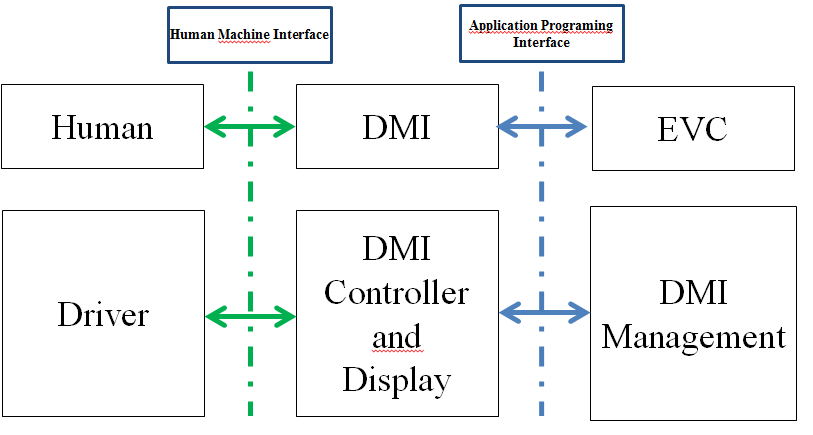
\includegraphics[width=.8\textwidth]{images/DMI_Interfaces}
  \caption{DMI Interfaces}
  \end{figure}

  \paragraph{Interface}
  The DMI Controller has two interfaces. One between DMI Controller and DMI Display and one between DMI Controller and DMI Management. 
  The structure of the interface between DMI Controller and DMI Display is driven by the logic of SCADE Display therefore It doesn't follow any standard or constraints (It will not be described in this chapter).
  DMI Controller and DMI Management exchange packets. Each packet is a structured type with a valid flag (a boolean variable), the DMI controller takes into account the data inside the packet only when the valid flag is true.

  The interface between DMI Controller and DMI Management consist of three parts according with the direction of the information:
  
  \begin{itemize}
  \item From DMI Management to DMI Controller
  \item From DMI Controller to DMI Management 
  \item Both ways directions (You will find the same type both as input than as output)
  \end{itemize}
  


\subparagraph{From DMI Management to DMI Controller}

In the following table are listed the inputs coming from DMI Management with a brief description:\\
  %\begin{table}[H]
    \begin{tabular}{| c | l | l | l | l |}
      \hline
      \textbf{NAME} & \textbf{DESCRIPTION} \\ \hline
      \texttt{DMI\_entry\_request} & Request to input data (e.g. driver id, Train running number etc.)\\
      \texttt{DMI\_identifier\_request} & Request of the DMI informations\\
      \texttt{DMI\_menu\_request} & Request to enable or disable buttons\\
      \texttt{DMI\_dynamic} & Contains informations about current speed, current mode etc.\\
      \texttt{DMI\_text\_message} & Contains predefined or plain text messages\\
      \texttt{DMI\_icons} & Request to display one or more icons in any area\\

      \hline
    \end{tabular} 
  % \caption{Overview of input}
    \label{tbl:DMICtrToDMIMng}
  %\end{table}
  
      Please note: TIU\_trainStatus input is missing in the above table. This is the only input coming directly from TIU and contains the open/close Desk signal. 
    
  \subparagraph{From DMI Controller to DMI Management}
  In the following table are listed the outputs directed to DMI Management with a brief description:\\
  %\begin{table}[H]
    \begin{tabular}{| c | l | l | l | l |}
      \hline
      \textbf{NAME} & \textbf{DESCRIPTION} \\ \hline
      \texttt{DMI\_identifier} & Information about DMI (e.g. version, cabin identifier etc.)\\
      \texttt{DMI\_driver\_request} & Driver request or acknowledgement\\
      \texttt{DMI\_train\_data\_ack} & Train data acknowledgement\\
      \texttt{DMI\_status\_report} & The actual status of DMI (keep alive)\\
      \texttt{DMI\_text\_message\_ack} & Text message acknowledgement\\
      \texttt{DMI\_icons\_ack} & Icon acknowledgement\\

      \hline
    \end{tabular} 
  % \caption{Overview of input}
    \label{tbl:DMICtrToDMIMng}
  %\end{table}
    
\subparagraph{Both ways direction}
In the following table are listed the outputs/inputs  to/from DMI Management with a brief description:\\
  
  %\begin{table}[H]
    \begin{tabular}{| c | l | l | l | l |}
      \hline
      \textbf{NAME} & \textbf{DESCRIPTION} \\ \hline
      \texttt{DMI\_driver\_identifier} & Contains the default or entered driver identifier\\
      \texttt{DMI\_train\_running\_number} & Contains the default or entered train running number\\
      \texttt{DMI\_train\_data} & Contains the default or entered train data\\
      \hline
    \end{tabular} 
  % \caption{Overview of input}
    \label{tbl:DMICtrToDMIMng}
  %\end{table}
  

\paragraph{Functional Design Description}
  \textbf{Please note}: \textit{DMI Controller is a project under construction, a lot of features and functionalities are missing, therefore the structure described below is a draft version and will be changing in the future.}
  
  The informations (received and sent) could be divided in two groups: Sporadic and Periodic. The first one are received/sent aperiodically in any time instead the second one are received/sent periodically, with a fixed deadline. Are part of Periodic group the output DM\_status\_report and the input DMI\_dynamic all other are Sporadic. Therefore, the structure of DMI Controller module consists of a first main state machine \textit{CabinSM} (Fig. \ref{fig:CabinSM}) triggered by  a \textit{OpenDesk} signal (from TIU). Inside the \textit{DeskIsOpen} state there are other two state machines :\textit{HandshakeSM} and \textit{DynamicInfoSM} (Fig. \ref{fig:DynSporSM}).
  
  HandshakeSM performs an initial handshake between DMI Controller and DMI Management. Before that, no data has to be sent or received to/from DMI Management. When the transition is fired a DMI\_identifier packet is sent to DMI Management with informations about the DMI (e.g. DMI identifier, DMI name etc.). At this point the DMI Controler is ready to manage the sporadic information (e.g. Enter or revalidate DriverID, Enter or revalidate Train running number etc.). 
  
  The DynamicInfoSM state machine is triggered after the handshake, exactly when  HandshakeSM reaches the  DynInfo\_Activated state. At the time when the transition is fired a signal is emitted (startDMI\_status) and begins a periodic sending of DMI status information (keep alive) to DMI Management. Once reached DynamicInfo\_Active, the DMI Controller is ready to receive and manage the dynamic informations.
  
   \begin{figure} 
      	\centering
      	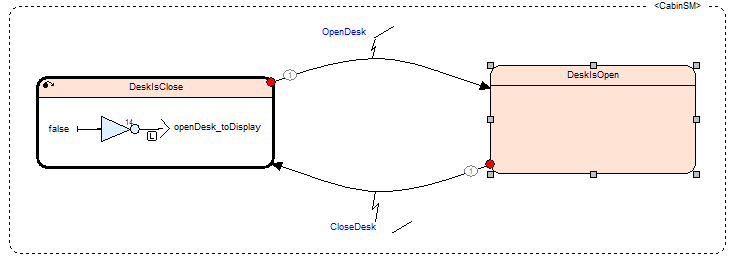
\includegraphics[scale=0.7]{images/CabinSM}
      	\caption{Cabin State Machine.}
      	\label{fig:CabinSM}
   \end{figure}
      
  \begin{figure} 
  \centering
  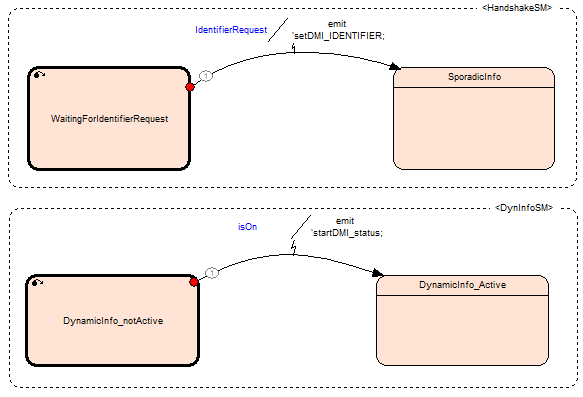
\includegraphics[scale=0.8]{images/DynSporInfoSM}
  \caption{HandshakeSM and DynamicInfoSM State Machines.}
  \label{fig:DynSporSM}
  \end{figure}
  


  With the aim to improve the readability and for a better management of complexity, all the functions (modules, state machines etc.) implemented in each state are divided several diagrams.
  
  The \textit{SporadicInfo} consist of:
  \begin{itemize}
  	\item \textbf{diagram\_SporadicInfo\_Main}: Contains all the modules to manage the sporadic data like ``Enter revalidate Driver ID'', ``Enter or revalidate train running number'', enable buttons in menus. The WindowSM state machine manages the windows that should appear on the DMI(Fig. \ref{fig:win_sm}).
  	
  	\item \textbf{ diagram\_SporadicInfo\_TrainData}: Contains all the logic to store and adapt the incoming train data to a correct visualization on DMI Display.
  	
  	\item \textbf{diagram\_SporadicInfo\_Icon\_Management}: Contains the logic to show/hide one or several icons in area and manage the acknowledgement mechanism if It's required.
  	
  	\item \textbf{ diagram\_SporadicInfo\_DriverID\_TRN}: Contains the logic to store and sent the Train running number and the Driver ID.
  	
  	\item \textbf{diagram\_SporadicInfo\_Text\_Messages}: Contains the modules, state machines and all the logic to manage and display predefined and customized text messages.
  \end{itemize}
  
  The \textit{ DynamicInfo\_Active} state consists of:\\
  
  \begin{itemize}
  	\item \textbf{diagram\_DynamicInfo\_Main}: Contains modules to store and display the informations like the current mode, ETCS level, RBC connection status and location brake target.
  	\item \textbf{diagram\_SpeedSupervision}: Contains the module where are implemented the behaviour of the speed pointer and the circular speed gauge ( informations about speed target, speed permitted and speed release).
  \end{itemize}
  
  \begin{figure}
  	\centering
  	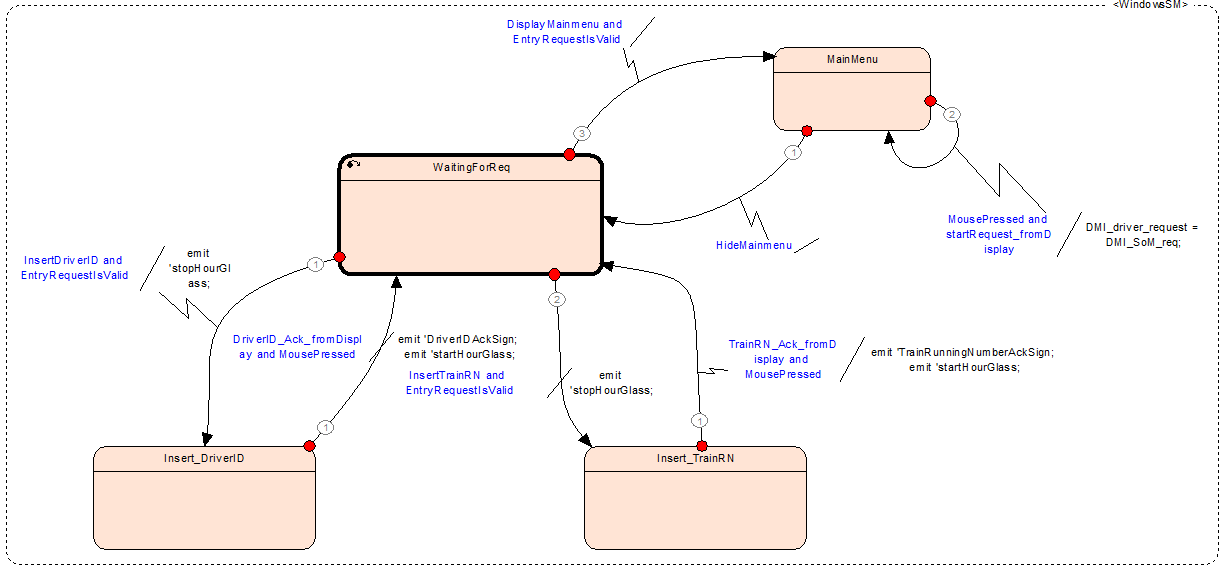
\includegraphics[width=\textwidth]{images/WindowSM}
  	\caption{Windows state machine.}\label{fig:win_sm}
  \end{figure}
  
\paragraph{Communication Protocol}
This section explains which messages are exchanged among DMI Controller, DMI Management and Start of mission procedure. As mentioned previously the DMI Controller is a passive component, It simply responds to requests, therefore is able to cover different scenarios. Below are some examples.
  
  \subparagraph{ Start Of Mission scenario} Are detailed, through a sequence diagram, all the activities (exchanged messages) that should be done to start. In this scenario we have three actors: DMI Controller, DMI Management and SoM procedure (the module where is implemented the start of mission procedure). It's assumed that a OpenDesk signal is received and the system starts in Stand By mode (Fig. \ref{fig:SeqDiaSoM}).
 
  \begin{figure}
  \centering
  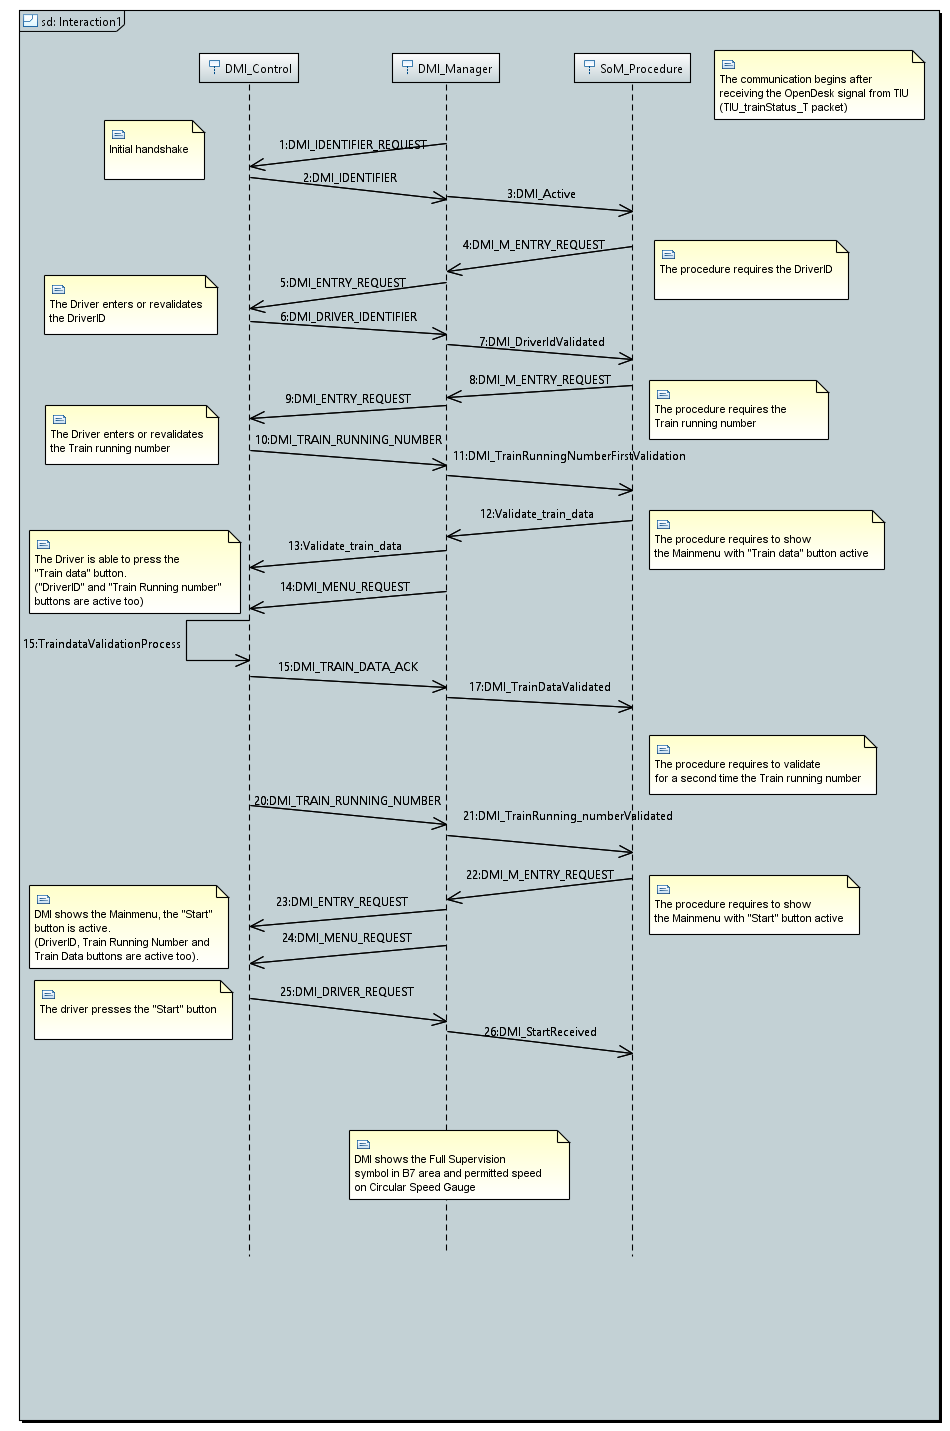
\includegraphics[scale=0.45]{images/SeqDia_DMIctr_DMImng_SoMproc}
  \caption{Sequence Diagram of start of mission scenario}\label{fig:SeqDiaSoM}
  \end{figure}
  

\subparagraph{ Cyclic Exchange of messages}
The time between two messages has not yet been definitively established, It might change in the future. The DMI status packet implements a keep alive mechanism, this means, if the EVC does not receive any DMI status signal during the lapse time, It shall consider a failure in DMI. This check is not yet implemented.

    \begin{figure}
      \centering
      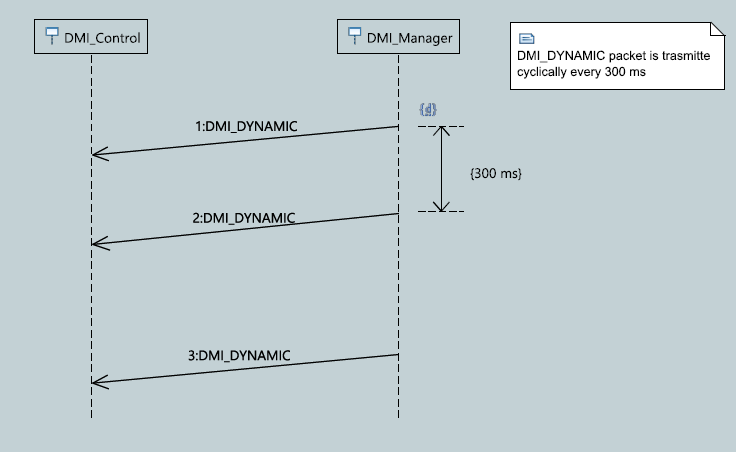
\includegraphics[scale=0.5]{images/DynamicPacket_SeqDia}
      \caption{ Sequence diagram of Dynamic data.}\label{fig:SeqDiaDyn}
    \end{figure}
  
    \begin{figure}
      \centering
      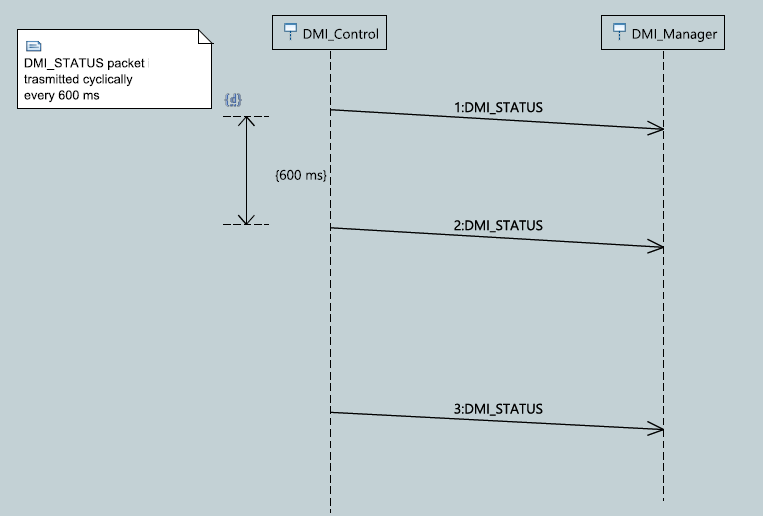
\includegraphics[scale=0.5]{images/DMIStatus_SeqDia}
      \caption{Sequence Diagram of DMI status.}\label{fig:SeqDiaStatus}
     \end{figure}
     

\paragraph{Reference to the Scade Model}

The SCADE model can be found on github under the following path: \url{https://github.com/openETCS/modeling/tree/master/model/Scade/System/DMI_Control}


\bibliographystyle{unsrt}
\bibliography{architecture}


\newpage
\addcontentsline{toc}{chapter}{Index}
\printindex
%===================================================
%Do NOT change anything below this line

\end{document}
